
\documentclass[openany]{report}
\usepackage[margin=1.2in]{geometry}
\usepackage{graphicx}
\usepackage{parskip}
\usepackage{fancyhdr}

\pagestyle{fancy}
\fancyhf{}                      % Clear all header and footer fields
\fancyhead[R]{\leftmark}        % Display chapter name at the top right corner

\title{C++ Workbook}
\author{Mikael J. Gonsalves}
\date{\today}
\begin{document}
\maketitle
\tableofcontents

\chapter{C++ Basics}

\section{Variables}

\begin{verbatim}
    int: integers                   // 4 bytes
    double: floating-point numbers  // double 8 bytes
    char: individual characters     // 1 byte
    float:                          // 4 bytes
    long:                           // 4 or 8 bytes (platform dependent)
    long long:                      // 8 bytes
    bool: true/false                // 1 byte

    // use sizeof for size

std::cout << "Size of int: " << sizeof(numInt); 
\end{verbatim}

\section{Auto}

Automatic deduction of value types. Standard c++11

\begin{verbatim}
constexpr double calculate_pi() {
    return 22/7;
}

constexpr auto pi = calculate_pi();

int main()
{
    const auto radius = 1.5;
    const auto area = pi * radius * radius;
    std::cout << area;

}

constexpr auto calculate_pi() {
    return 22/7;
}

constexpr auto pi = calculate_pi();

// east/ west const
const auto result = std::count( /*stuff */);
auto const result = std::count( /*stuff*/ );
\end{verbatim}


\section{Constexpr}

Compile-time generation of code and data. Compile-time constant.

\begin{verbatim}
const double pi = 3.141593;

int main()
{
   const double radius = 1.5;
   const double area = pi * radius * radius;
   std::cout << area;
}

constexpr double pi = 3.141593;

int main()
{
   const double radius = 1.5;
   const double area = pi * radius * radius;
   std::cout << area;
}
\end{verbatim}

\subsection{Overcomplicated Constexpr}

\begin{verbatim}

// static const data known at compile time. 
static const std::vector<int> angles{-90,-45,0,45,90};
\end{verbatim}

\subsection{Useful Constexpr}

\begin{verbatim}
// Moving static const to static constexpr.
static constexpr std::array<int, 5> angles{-90,45,0,45,90};

Here static constexpr makes sure the object
is not reinitialized each time the function is encountered.

\end{verbatim}

\section{Const Char}

\begin{verbatim}
#include <filesystem>
namespace fs = std::filesystem;

int main() {
    fs::path path = "your_directory_path";

    for (const auto &entry : fs::directory_iterator(path)) {
        const char *cstr = entry.path().c_str();
        std::cout << cstr << '\n';
    }
    return 0; // return success
}
\end{verbatim}

\section{Synthax}
\subsection{Ternary Operator}
\begin{verbatim}
std::cout << (coin == 0 ? "Heads" : "Tails") << "\n";
\end{verbatim}

\subsection{Relational Operators}

\begin{verbatim}
    ==              equal to
    !=              not equal to
    >               greater than
    <               less than
    >=              greater than or equal to
    <=              less than or equal to
\end{verbatim}

\subsection{Logical Operators}

\begin{verbatim}
    &&              and 
    ||              or
    !               not

    if (hunger && anger){}

    ( !true )       not false
    ( !(10 < 11) )  not condition 
\end{verbatim}

\subsection{String Manipulation}

\begin{verbatim}
reversed_text += text

std::string chapOnePath = parentDirectory + "/chap_1";
\end{verbatim}

\subsection{Scope}

\begin{verbatim}
run() {
    {
        Is this in scope? //This variable is out of scope.?
    {
    
}
\end{verbatim}

\subsection{Chaining}

\begin{verbatim}
int age = 28;
std::cout << age << "years old.\n";

template <typename T>
struct MathOperation {
    T value;

    MathOperation(T val) : value(val) {}

    template <typename U>
    MathOperation<U> add(U val) {
        return MathOperation<U>(value + val);
    }

    template <typename U>
    MathOperation<U> multiply(U val) {
        return MathOperation<U>(value * val);
    }

    void print() {
        std::cout << "Result: " << value << std::endl;
    }
};

int main() {
    MathOperation<int> operation(5);
    operation.add(3).multiply(2).print();

    return 0; // return success
}
\end{verbatim}

\section{Streams}

\begin{verbatim}
    std::cin            : Standard input stream for reading user input.
    std::cout           : Standard output stream for writing output.
    std::cerr           : Standard error stream for writing error messages (unbuffered).
    std::clog           : Standard error stream for writing log messages (buffered).
    std::ifstream       : Input file stream for reading from files.
    std::ofstream       : Output file stream for writing to files.
    std::fstream        : File stream for reading from and writing to files.
    std::istringstream  : Input string stream for reading from strings.
    std::ostringstream  : Output string stream for writing to strings.
    std::stringstream   : String stream for reading from and writing to strings.
    std::wcin           : Wide character version of std::cin for reading wide characters.
    std::wcout          : Wide character version of std::cout for writing wide characters.
    std::wcerr          : Wide character version of std::cerr for writing wide error messages.
    std::wclog          : Wide character version of std::clog for writing wide log messages.
\end{verbatim}

\subsection{Sstream}

`std::stringstream` is a C++ class. It handling string-based input and output operations,
allowing you to read from and write to strings as if they were input/output streams.

\begin{verbatim}
#include <map>
#include <sstream>

int main() {
    std::string text = "lorem";

    for (char& c : text) {
        c = std::tolower(c);
    }

    std::map<std::string, int> wordfreq;
    std::istringstream iss(text);
    std::string word;

    while (iss >> word) { // count frequency
        wordfreq[word]++;
    }

    for (const auto& pair : wordfreq) { // display
        std::cout << pair.first << ": " << pair.second;
    }

    return 0; // return success
}
\end{verbatim}


\section{Touples}


\section{Enums}

\begin{verbatim}
enum class Day {
    Monday,
    Tuesday,
    Wednesday,
};

int main() {
    Day today = Day::Tuesday;

    if (today == Day::Saturday || today == Day::Wednesday) {
    } else {}

    return 0; // return success
}

enum Color {
    Red,
    Green,
    Blue
};

void printColor(Color color) {
    switch (color) {
        case Red:
            break;
        case Green: // ...
            break;
        case Blue: // ...
            break;
    }
}

int main() {
    Color favoriteColor = Color::Green;
    printColor(favoriteColor);

    return 0; // return success
}
\end{verbatim}

\subsection{Enum Array Mapping}

\begin{verbatim}
enum class Fruit {
    Apple,
    Banana,
    Orange
};

const std::array<std::string, 3> fruitNames = {
    "Apple",
    "Banana",
    "Orange"
}

const std::string fruitNames[] = { // c-style array
                                   // size by initializer
    "Apple",
    "Banana",
    "Orange"
};

int main() {
    Fruit selectedFruit = Fruit::Banana;
    int fruitIndex = static_cast<int>(selectedFruit);

    std::cout << "Selected fruit: " << fruitNames[fruitIndex] << std::endl;

    return 0; // return success
}
\end{verbatim}

\subsection{Enum Vector Mapping}

\begin{verbatim}
enum class Month {
    January,
    February,
    March // ...
};

const std::vector<std::string> monthNames = {
    "January",
    "February",
    "March" // ... 
};

int main() {
    Month currentMonth = Month::May;
    int monthIndex = static_cast<int>(currentMonth);

    std::cout << "Current month: " << monthNames[monthIndex] << std::endl;

    return 0; // return success
}
\end{verbatim}


\section{Arrays}

A fixed-size stack-based container. Having the size type information gives more optimization oppotunities.

\begin{verbatim}
#include <array> // c++ 11
    std::array<char, 128> second = {'H', 'e', 'l'} // from library
                            // fixed size of 128
                            // has .begin(), .end(), .at(), .size() 

    sint arr[] = {1, 2, 3}; // c-style array 
                            // size determined by initializer's list
                            // fixed at compile-time 

std::array<Type, Size> data

#include <numeric>
#include <array>

template<typename Value_Type>
std::array<Value_Type, 3> get_data(const Value_Type &v1, const Value_type &v2,
                                   const Value_type &v3)
{
    std::array<Value_Type 3> data;
    data[0] = v1;
    data[1] = v2;
    data[2] = v3;
    return data;
}

// no dynamic allocation, 
// win-win scenario with knowing the size of the data struture at compile time.

template<typename> VT> // takes 3 parameters
std::array<VT, 3> get_data(const VT &v1, const VT &v2, const VT &v3)
{
    return {v1, v2, v3};
}

template<typename> VT> // takes 4 parameters
std::array<VT, 4> get_data(const VT &v1, const VT &v2, const VT &v3, const VT &v4))
{
    return {v1, v2, v3, v4};
}
\end{verbatim}

\subsection{Dynamic Array Allocation}

Achieved using pointers and dynamic memory allocation operators, such as `new` and `delete`. 
While arrays are considered static containers,
dynamic arrays allow you to allocate memory at runtime.

\begin{verbatim}
int size = 5; // desired size of the array
int* dynamicArray = new int[size]; // allocate memory for the array

// Access and modify elements of the dynamic array
dynamicArray[0] = 10;
dynamicArray[1] = 20;
// ...

// Deallocate the memory when it's no longer needed
delete[] dynamicArray;

#include <array>

int main() {
    std::array<int, 3> ar{1,2,3};

    int* dyn_ar = new int[4];

    dyn_ar[0] = 10;
    dyn_ar[1] = 20;
    dyn_ar[2] = 30;
    dyn_ar[3] = 40;
    dyn_ar[4] = 50;
    dyn_ar[5] = 60;
    dyn_ar[6] = 70;

    for (int i = 0; i < 7; i++) {
        std::cout << dyn_ar[i] << " ";
    }
    std::cout << std::endl; // prints 10, 20, 30, 40.. 70.

    delete[] dyn_ar;

    return 0; // return success
}

\end{verbatim}

`new int[size]` dynamically allocates memory. 
`delete[] dynamicArray` deallocates the memory to avoid memory leaks.

Alternatively, using smart pointers or container classes like `std::vector` can help automate memory management
and provide safer alternatives for dynamic arrays.

\section{Vectors}

Vectors are \textbf{dynamic array-like container that can grow or shrink.}

\begin{verbatim}
  std::vector<double> subway_adult; // value is 0.0 is default
  std::vector<double> location(2); // initialize two elements! 
}

std::vector<char> vowels = {'a', 'e', 'i', 'o', 'u'};
std::vector vec{1,2,3}; // now possible! 

int main(int argc, char* argv[]) {
    std::vector<std::string> arguments(argv + 1, argv + argc);
}

template<typename Value_Type>
std::vector<Value_Type> get_data(const Value_Type &v1, const Value_Type &v2,
                                 const Value_Type &v3)

{
    std::vector<Value_Type> data;
    data.push_back(v1);
    data.push_back(v2);
    data.push_back(v3);
    return data;
}
\end{verbatim}

\section{Size\_t}

\begin{verbatim}
template<typename Value_Type>
struct Data {
    Data(const std::size_t size)
      : data(new Value_Type[size]) // constructor
    {
    }

    ~Data() { delete [] data; }

    Value_Type *data;
};
\end{verbatim}

In the `Data` struct, the constructor takes a `std::size\_t` parameter named `size`,
which specifies the desired size of the `data` array. 
By using `std::size\_t` as the parameter type, 
it ensures that the value provided for `size` is appropriate for representing the size of the array.

Inside the constructor, the `data` member is \textbf{allocated dynamically using `new`}.

The size of the array is specified as the value of `size`, which is of type `std::size\_t`. 
This ensures that the correct amount of memory is allocated for the array based on the given size.

\section{Iterators}
\subsection{Conditionals}

\begin{verbatim}
if (coin == 0) {
} else {}
}
\end{verbatim}

\subsection{Switch Statements}

\begin{verbatim}
int main() {
  int number = 9;
  switch(number) {
    case 1 : // ...
      std::cout << "case one";
      break;
    case 2 :
      break;
    default : // ...
      break;
  }
}
\end{verbatim}

\subsection{Loops}

\begin{verbatim}
while (guess != 8) {
  std::cout << "Wrong guess, try again: ";
  std::cin >> guess;
}

for (int i = 0; i < 20; i++) {}  // incrementing
for (int i = 20; i > 0; i--) {}  // decrementing
\end{verbatim}

\section{Ranges}

\begin{verbatim}
#include <format>
#include <string_view>

void print_map(const auto &map,
               const std::string_view &key_desc = "key",
               const std::string_view &value_desc = "value")
{
    const auto print_key_value = [&](const auto &data) { 
        const auto &[key, value] = data;
        std::puts(std::format("{}: '{}' {}: '{}'",
                         key_desc, key, value_desc, value).c_str());
    };

    for_each(map, print_key_value);
}

#include <ranges>

int main()
{
    std::vector<int> ints{1, 2, 3, 4, 5};
    auto even = [](int i){ return 0 == i % 2; };
    auto square = [](int i){ return i * i; };
                                              
    for (int i : ints | std::view::filter(even) | std::view::transform(square)) {
        std::cout << i << ' ';
    }
}
\end{verbatim}

\subsection{Ranges Pipes}

I are operators for composing ranges in C++20.

They chain range adaptors, transforming or filtering operations.
Pipes take the output of one range and passes it as the input to the next range adaptor,
allowing you to compose multiple operations on a range in a concise and readable way.

\begin{verbatim}
auto even = [](int i){ return 0 == i % 2; };
auto square = [](int i){ return i * i; };

for (int i : ints | std::view::filter(even) | std::view::transform(square)) {
    std::cout << i << ' ';
}

`ints`: The input range of integers.
`std::view::filter(even)`: Filters the `ints` range, keeping only the even numbers.
`std::view::transform(square)`: Transforms the filtered range by squaring each element.
`int i : ...`: Iterates over the resulting transformed range and assigns each element to `i`.
`std::cout << i << ' ';`: Prints each element `i` separated by a space.
\end{verbatim}

\subsection{Range-Based for Loops}


Iterate over container elements (array, vector or std::list). It doesn't work for forward\_list.


Works with anything that has begin()
and end() members/functions, C-Style arrays and initializer lists.

\begin{verbatim}

for (const auto &element : container) {}

std::string str = "Hello";
for (char character : str) {
    std::cout << character << '\n';
}

template<typename Map>
void print_map(const Map &map, const std::string &key_desc = "key",
                               const std::string &value_desc = "value")
{
    for (const auto &data : map)
    {
        std::cout << key_desc << ": '" << data_itr->first << "' "
                  << value_desc << ": '" << data_itr->second << "'\n";
    }
}

for (const auto &value : container) {} // for each element in the container

Use clang-tidy's modernize-loop-convert check.

template<typename Map>
void print_map(const Map &map, const std::string &key_desc = "key",
                               const std::string &value_desc = "value")
{
    for (const auto &data : map)
    {
        std::cout << key_desc << ": '" << data.first << "' "
                  << value_desc << ": '" << data.second << "'\n";
    }
}
\end{verbatim}

\subsection{Accidental Conversions}

\begin{verbatim}
for (const int value : container_of_double) {
    // accidental conversion, possible warning
}
\end{verbatim}

\subsection{Accidental Slicing}

\begin{verbatim}
for (const base value : container_of_derived) {
    // accidental silent slicing
}

If container_of_derived holds objects of a derived class. 
Base is the base class.
The loop is iterating over the container and assigning each
derived object to a base object (value) due to object slicing.

Object slicing occurs because the base object can only store
the base class's attributes and behavior. Additional defined 
class attributes will be lost during the assignment or copy.

To avoid accidental slicing, you use pointers or references.

// no problem
for (const auto &value : container) {
    // no possible accidental conversion
}

Using pointers or references ensures that 
the derived objects retain their specific attributes and behavior.

const auto & for non-mutating loops
auto & for mutating loops
auto && 
// only when you have to with weird types like std::vector<bool>,
// or if moving elements out of the container
\end{verbatim}

\section{Functions}

\begin{verbatim}
void eat() {
  std::cout << "nom nom\n";
}

bool even(int num) {
  return ( num % 2 == 0 ? true : false );
  // this should be tested
}
\end{verbatim}

\subsection{Inline Functions}

The compiler inserts the function’s body on the function call.

\begin{verbatim}
inline 
void eat() {
  std::cout << "nom nom\n";
}

-- single line in header file is slower --
void Cookie::eat() {std::cout << "nom nom\n";}

-- goodnight.cpp --
std::string goodnight1(std::string thing1) {
  return "Goodnight, " + thing1 + ".\n";
}
-- goodnight.h --
std::string goodnight1(std::string thing1);

-- night.hpp -- 
inline
std::string goodnight1(std::string thing1) {
  return "Goodnight, " + thing1 + ".\n";
}
\end{verbatim}

\subsection{Class Functions (Member Functions)}

Functions inside of classes.

\begin{verbatim}
class Musician {
private:
    int instruments;

public:
    int getMyVariable() const {
        return myVariable;
    }

    void setMyVariable(int newValue) {
        myVariable = newValue;
    }
};

int main() {
    MyClass obj;
    obj.setMyVariable(42);

    int value = obj.getMyVariable();
    return 0;
}
\end{verbatim}

\subsection{Functions Public}

\begin{verbatim}
class City {
  int population; 
 
public:         // accessible outside of the class
  void add_resident() { 
    population++;
  }

private:        // private to this class
  bool is_capital;
};

-- song.h --
class Song {
  std::string title;
  std::string artist;

public:
  void add_title(std::string new_title);
  std::string get_title();
  
  void add_artist(std::string new_artist);
  std::string get_artist();
};

-- song.cpp --
#include "song.hpp"

void Song::add_title(std::string new_title) {
  title = new_title;
}

std::string Song::get_title() {
  return title;
}

void Song::add_artist(std::string new_artist) {
  artist = new_artist;
}

std::string Song::get_artist() {
  return artist;
}

-- city.h -- 
#include "city.hpp"
 
class City {
  std::string name;
  int population;
 
public:
  City(std::string new_name, int new_pop);
 
};

-- city.cpp --
City::City(std::string new_name, int new_pop)
  : name(new_name), population(new_pop) {} 

-- main.cpp --
City ankara("Ankara", 5445000);

-- song.h -- 
class Song {
  std::string title;
  std::string artist;

public:
  Song(std::string new_title, std::string new_artist);

  void add_title(std::string new_title);
  std::string get_title();

  void add_artist(std::string new_artist);
  std::string get_artist();
};

-- song.cpp --
#include "song.hpp"

Song::Song(std::string new_title, std::string new_artist)
  : title(new_title), artist(new_artist) {}

void Song::add_title(std::string new_title) {
  title = new_title;
}

std::string Song::get_title() {
  return title;
}

void Song::add_artist(std::string new_artist) {
  artist = new_artist;
}

std::string Song::get_artist() {
  return artist;
}

-- song.h --

class Song {
  std::string title;
  std::string artist;

public:
  Song(std::string new_title, std::string new_artist);

  std::string get_title();
  std::string get_artist();
};

-- song.cpp --
#include "song.hpp"

Song::Song(std::string new_title, std::string new_artist)
  : title(new_title), artist(new_artist) {}

std::string Song::get_title() {
  return title;
}

std::string Song::get_artist() {
  return artist;
}

-- main.cpp --
#include "song.hpp"

int main() { 
  Song back_to_black("Back to Black", "Amy Winehouse");

  std::cout << back_to_black.get_title() << "\n";
  std::cout << back_to_black.get_artist() << "\n";
}
\end{verbatim}

\subsection{Functions Overloading}

Accepts many types as parameters.

Change behavior based on parameter's type.

\begin{verbatim}
// one must be true
    Each has different type parameters.
    Each has a different number of parameters.
    
-- num.cpp --
int fancy_number(int num1, int num2) {
  return num1 - num2 + (num1 * num2);
}

int fancy_number(int num1, int num2, int num3) {
  return num1 - num2 - num3 + (num1 * num2 * num3);
} // different number of params.

int fancy_number(double num1, double num2) {
  return num1 - num2 + (num1 * num2);
}               // different type of params.

-- num.hpp --
int fancy_number(int num1, int num2);
int fancy_number(int num1, int num2, int num3);
int fancy_number(double num1, double num2);
\end{verbatim}

\section{Parameters}

\begin{verbatim}
void get_emergency_number(std::string emergency_number) {}

struct ComplexType {
    int value;
    std::vector<int> data;
};

void processComplexType(const ComplexType& complexParam) {
    std::cout << "Value: " << complexParam.value << std::endl;
    std::cout << "Data:";
    for (int num : complexParam.data) {
        std::cout << " " << num;
    }
    std::cout << std::endl;
}

int main() {
    ComplexType complexObj;
    complexObj.value = 42;
    complexObj.data = {1, 2, 3, 4, 5};

    processComplexType(complexObj);

    return 0;
}

Many Parameters

double get_tip(double price, double tip, bool total_included) {
    get_tip(0.25, true, 45.50); // will not work. Order matters. 
}

void name_x_times(std::string name, int x){
  while (x > 0) {
    std::cout << name << "\n";
    x--;
  }
}
\end{verbatim}

\subsection{Pass-By-Value}

Passing by value makes modification impossible, since the passed variable is out of scope.
Pass by reference to modify the passed parameter.

\begin{verbatim}
void useless_function(int val) {
    val = val * 2;
}
\end{verbatim}


\subsection{Pass-By-Reference}

Modify the argument's value.
Avoid making copies of a variable/object for performance reasons.

\begin{verbatim}
void swap_num(int &i, int &j) {
  int temp = i;
  i = j;
  j = temp;
}
 
int main() {
  int a = 100;
  int b = 200;
 
  swap_num(a, b);
}

int triple(int &i) {
  i = i * 3;
  return i;
}

int main() {
  int num = 1;
  std::cout << triple(num) << "\n";
}

template<typename T>
void modifyVector(std::vector<T>& vec) {
    for (auto& element : vec) {
        element *= 2;
    }
}

template<typename T>
void printVector(const std::vector<T>& vec) {
    for (const auto& element : vec) {
        std::cout << element << " ";
    }
    std::cout << std::endl;
}

int main() {
    std::vector<int> numbers = {1, 2, 3, 4, 5};

    printVector(numbers);  // Output: Original vector: 1 2 3 4 5
    modifyVector(numbers);

    printVector(numbers);  // Output: Modified vector: 2 4 6 8 10
    return 0;
}
\end{verbatim}

\subsection{Parameters Default Values}

\begin{verbatim}
struct Chapters {
    bool IsToPrint = true;
};

struct Chapters {
    bool IsToPrint;

    Chapters() : IsToPrint(true) {} // with default constructor
};

int main() {
    Chapters c1;
    Chapters c2 = {false}; //  list initialization
                           // works when only one bool in struct

    // c1.IsToPrint will be true
    // c2.IsToPrint will be false

    return 0;
}
\end{verbatim}

\subsection{Default Arguments}

\begin{verbatim}
void intro(std::string name, std::string lang = "C++");
\end{verbatim}

\section{References}

\subsection{References Variables}

\textbf{A second name for an existing variable}.

\begin{verbatim}
int &sonny = songqiao; // Sonny, a reference to songqiao;

\\ Changes to the reference happens to the original.
\\ Aliases cannot be changed to alias something else.

  int soda = 99;
  int &pop = soda;
  pop++; // soda and pop equal at 100

Using a reference (&) instead of making a copy of the elements is more efficient,
especially when dealing with large objects or containers. 

By using a reference, the loop avoids creating a new copy of each element
, reducing unnecessary memory usage and improving performance.

struct ComplexStruct {
    int value1;
    int value2;
};

void modifyStruct(ComplexStruct& ref) {
    ref.value1 = 100;
    ref.value2 = 200;
}

int main() {
    int x = 10;
    int& ref1 = x;              // Reference variable ref1 refers to x
    ref1 = 20;                  // Modifying ref1 will also modify x

    ComplexStruct obj;
    obj.value1 = 50;
    obj.value2 = 60;
    ComplexStruct& ref2 = obj;  // Reference variable ref2 refers to obj

    modifyStruct(ref2);         // Modifying ref2 will also modify obj
    return 0;
}
\end{verbatim}

\subsection{Dereference}

Obtain the pointer's pointed value. 

\begin{verbatim}
Declaration? * creates a pointer.
Not a declaration? * is a dereference operator.

int main() {
  int power = 9000;
  int* ptr = &power;
  std::cout << *ptr; // prints 9000
}
\end{verbatim}

\subsection{Pass-By-Reference}

Now, when called, the function can modify the argument's value.
Avoid making copies of a variable/object for performance reasons.

\begin{verbatim}
//Calling swap_num(), variables a and b's value will be modified
//because they are passed by reference

void swap_num(int &i, int &j) {
  int temp = i;
  i = j;
  j = temp;
}
 
int main() {
  int a = 100;
  int b = 200;
 
  swap_num(a, b);
 
  std::cout << "A is " << a << "\n";
  std::cout << "B is " << b << "\n";
}

WHEN? To MODIFY the arguments’ values.

int triple(int &i) {
  i = i * 3;
  
  return i;
}

int main() {
  int num = 1;
  std::cout << triple(num) << "\n";
}

template<typename T>
void modifyVector(std::vector<T>& vec) {
    for (auto& element : vec) {
        element *= 2;
    }
}

template<typename T>
void printVector(const std::vector<T>& vec) {
    for (const auto& element : vec) {
        std::cout << element << " ";
    }
    std::cout << std::endl;
}

int main() {
    std::vector<int> numbers = {1, 2, 3, 4, 5};

    std::cout << "Original vector: ";
    printVector(numbers);  // Output: Original vector: 1 2 3 4 5

    modifyVector(numbers);

    std::cout << "Modified vector: ";
    printVector(numbers);  // Output: Modified vector: 2 4 6 8 10

    return 0;
}
\end{verbatim}

\subsection{References Const}

\begin{verbatim}
int triple(const int &i) { // save computational cost
  return i * 3;            // don't make a copy of the argument
}

int square(const int &i) {
  return i * i;
}

int main() {
  int side = 5;
  std::cout << square(side) << "\n";
}
\end{verbatim}

\subsection{Reference Operator}

\begin{verbatim}
int soda = 99; 
int &pop = soda;
pop++;
\end{verbatim}

\subsection{Address Operator}

\begin{verbatim}
int porcupine = 3; 
std::cout << &porcupine << "\n"; 

// 0x7ffd7caa5b54
\end{verbatim}

\chapter{Memory Allocation}
\section{Pointers}

\begin{verbatim}
Declaration? * creates a pointer.
Not a declaration? * is a dereference operator.

int main() {
  int power = 9000;
  int* ptr = &power;
  std::cout << *ptr; // prints 9000
}

int* number;         // Declaring
double* decimal;
char* character;

int gum = 8;
int* ptr = &gum;     // int* [declare a pointer]
                     // ptr [pointer's name]
                     // &gum [store gum's memory address in ptr]

int* number;         // Declaration standard
int *number;
int * number;        // All Synthaxically valid

\end{verbatim}

\subsection{Null Pointers}

Ptr to a yet unknown memory address.

\begin{verbatim}
int* ptr; // declared, not yet initialized
\end{verbatim}

\subsection{Nullptr}

Type safe pointer since C++14, I think. A replacement for NULL.

\begin{verbatim}
int* ptr = nullptr;
\end{verbatim}


\subsection{Unique Pointers}

\begin{verbatim}
class Factory {
public:
    std::unique_ptr<Product> createProduct(const std::string& productType) {
        if (productType == "A") {
            return std::make_unique<ConcreteProductA>();

            // make unique
            // create an instance of std::unique_ptr


        } else if (productType == "B") {
            return std::make_unique<ConcreteProductB>();
        } else {
            return nullptr;
        }
    }
};

#include <memory>

int main() {
    std::unique_ptr<int> num_ptr = std::make_unique<int>(42);
    // num_ptr owns the dynamically allocated integer

    // ...
    
    return 0;
}

\end{verbatim}

\subsection{Smart Pointers}

\subsection{Pointer of Pointer}

\begin{verbatim}
int main() {
    int value = 5;
    int* ptr = &value;
    int** ptrToPtr = &ptr;

    return 0;
}
\end{verbatim}

\subsection{Allocation}

\subsection{Deallocation}

\subsection{Freeing Memory}
\subsection{Leaking Memory}

\section{Classes}

\begin{verbatim}
A C++ class is a user-defined type.

class City {
}; // needs semicolon
\end{verbatim}

\subsection{Class Components}

\begin{verbatim}
Class components are called class members
Attributes and methods are class members

class City {
  int population; // attribute
 
public:
  void add_resident() { // method
    population++;
  }
};
\end{verbatim}


\section{Span}

A non-owning, lightweight and flexible view over a contiguous sequence of elements.
A `span` is a pointer to the first element and the number of elements in the sequence.
A non-owning view, \textbf{it can be used to work with the array without copying its elements}.

Pass and manipulate data ranges, such as sub-arrays or portions of containers,
without memory allocation overhead or ownership.

It allows you to write generic functions that operate on different containers
without requiring specific container types.

\begin{verbatim}
#include <span>

void printSpan(std::span<int> sp) {
    for (int element : sp) {}
}

int main() {
    std::array<int,5> arr{1, 2, 3, 4, 5};
    std::span<int> span(arr, 5);

    printSpan(span); // takes span and prints elements
    return 0;
}
\end{verbatim}

\section{Templates}

The ultimate in the DRY principle. Write a template that has types and values filled in at compile-time.

\begin{verbatim}
template <typename meaningful_Type>
meaningful_Type get_smallest(meaningful_Type num1, meaningful_Type num2) {
  return num2 < num1? num2 : num1;
}

int main() {
  std::cout << get_smallest(100, 60) << "\n";
  std::cout << get_smallest(2543.2, 3254.3) << "\n";
}

template types are generated by the compiler at compile time
Do not need any kind of type-erasure (like Java generics do)

Highly efficient runtime code possible, 
as good as (or better than) hand writing the various options
template system is Turing complete (not necessarily a good thing)

    template<typename SomeType>
    struct S { // struct can do anything it wants with this type
    };

// declare a class template that can hold anything we want
template<typename Value_Type>
struct Data {
    Data(const std::size_t size)
      : data(new Value_Type[size])
    {
    }

    ~Data() { delete [] data; }

    Value_Type *data;
};

// declare a function template that take 3 params of the same type
// and passes that type on to the 'Data' template

template<typename Value_Type>
Data<Value_Type> get_data(const Value_Type &v1, const Value_Type &v2,
                          const Value_type &v3)
{
    {Data<Value_Type> d(3);
    d.data[0] = v1; d.data[1] = v2; d.data[2] = v3;
    return d;
}
\end{verbatim}

\subsection{Templates Basics}

\begin{verbatim}
template<typename T>
T divide(T numerator, T denominator) {
    return numerator / denominator;
}
\end{verbatim}

\subsection{Variadic Templates}

Drastic simplification of code needing to match a variable number of parameters.

\begin{verbatim}
#include <array>

// require at least one parameter and it sets the type
template<typename VT, typename ... Params>
std::array<VT, sizeof...(Params)+1> get_data(const VT &v1, const Params& ...params)
{
    return {v1, params...};
}


template<typename VT, Typename ... P> // variadic template
std::array<VT, sizeof...(P)> get_data(const P & ... params) // param expansion
{
    return {params...}; // pack expansion
}

template<typename> VT>
std::array<VT, 3> get_data(const VT &v1, const VT &v2, const VT &v3) // 3 params
{
    std::array<VT, 3> data;
    data[0] = v1; data[1] = v2; data[2] = v3;
    return data;
}

template<typename> VT>
std::array<VT, 2> get_data(const VT &v1, const VT &v2) // 2 params
{
    std::array<VT, 2> data;
    data[0] = v1; data[1] = v2;
    return data;
}

template<typename> VT>
std::array<VT, 1> get_data(const VT &v1) // 1 params
{
    std::array<VT, 1> data;
    data[0] = v1;
    return data;
}

// This bothers.
template<typename Value_Type>
struct Data {
    Data(const std::size_t size)
      : data(new Value_Type[size])
    {
    }

    ~Data() { delete [] data; }

    Value_Type *data;
};
\end{verbatim}

\subsection{CTAD - Class Template Argument Deduction}

\begin{verbatim}
template<typename VT, typename ... Params>
auto get_data(const VT &v1, const Params & ... params)
{
    return std::array{v1, params...}; // auto deduced size/type
}

std::vector vec{1,2,3}; // now possible! 
and now we can simplify the template arguments

/include <array>

template<typename ... Params>
auto get_data(const Params & ... params)
{
    return std::array{params...};
}
\end{verbatim}

\subsection{Templates Auto Return Types}

\begin{verbatim}
template<typename Numerator, typename Denominator>
auto divide(Numerator numerator, Denominator denominator)
{
    return numerator / denominator;
}
\end{verbatim}


\subsection{Return Value Optimization}
RVO, a compiler optimization technique on 
unnecessary object copies when returning.


When a function returns an object by value,
the traditional behavior involves creating a temporary object to hold 
the returned value and then copying that temporary object to the caller's destination object.


RVO directly constructs the return value object in the memory allocated by the caller.
This avoids the temporary object creation and data copy.

\section{Structs}

The only difference between a struct and a class is public properties. With
structs, all properties are public by default.

\begin{verbatim}
struct Double_Data {
    Double_Data(const std::size_t size) : data(new double[size] { }
    ~Double_Data() { delete [] data; }
    double *data;
   };

// I want one for ints!
struct Int_Data {
    Int_Data(const std::size_t size) : data(new int[size] { }
    ~Int_Data() { delete [] data; }
    int *data;
   };

// I want one for floats!
struct Float_Data {
    Float_Data(const std::size_t size) : data(new float[size] { }
    ~Float_Data() { delete [] data; }
    float *data;
   };
\end{verbatim}

\subsection{Structs Against Classes}
\begin{verbatim}
The only difference between them is that struct has all members by default public.
Using struct makes examples shorter and easier to read. 
\end{verbatim}

\section{Lambdas}

Unnamed function objects occasionally capturing.

\begin{verbatim}
auto lambda = [/*captures*/](int param1){ return param1 * 10; };

std::vector<int> ints{1, 2, 3, 4, 5};
auto even = [](int i){ return 0 == i % 2; };
auto square = [](int i){ return i * i; }; 

for (int i : ints | std::view::filter(even) | std::view::transform(square)) {
    std::cout << i << ' ';
}
\end{verbatim}

\subsection{Lambdas Captures}

Access variables from its surrounding scope.
Used outside variable within their body.

The captures section can be left empty if
the lambda does not need to access any external variables.

\begin{verbatim}
auto lambda = [/*captures*/](int param1){ return param1 * 10; };
\end{verbatim}

\subsection{Lambdas Captures by Values}

A copy of the variable is made.

\begin{verbatim}
auto lambda = [param](int param1){ return param1 * 10; };
\end{verbatim}

\subsection{Lambdas Captures References}

\begin{verbatim}
auto lambda = [&param](int param1){ return param1 * 10; };
\end{verbatim}

\subsection{Lambdas Captures by Values and References}

Capture multiple variables, 

\begin{verbatim}
int x = 42;
double y = 3.14;

auto lambda = [x, &y](int param1){ return x * param1 + y; };

    // x is captured by value, creating a copy
    // y is captured by reference, with access to original
\end{verbatim}

\subsection{Lambda Auto}
\begin{verbatim}
template<typename Map>
void print_map(const Map &map, const std::string key_desc = "key",
                               const std::string value_desc = "value")
{
    for_each(begin(map), end(map),
        [&](auto &data) { /// Sick !!
                          /// This makes a generic lambda.
            std::cout << key_desc << ": '" << data.first << "' "
                      << value_desc << ": '" << data.second << "'\n";
            }
    );
}
\end{verbatim}

\subsection{Lambdas Generic Lambdas}

Create implicit templates by simply using the auto keyword.

\begin{verbatim}
auto lambda = [/*captures*/](auto ... params){
    return std::vector<int>{params...};
}

standard c++14
\end{verbatim}

\subsection{Lambdas Variadic}

\subsection{Lambdas Const Object Initionalization}

\begin{verbatim}
const auto data = [](){ // no parameters
    std::vector<int> result;
                        // fill result with things. 
    return result;
}();                    // immediately invoked
\end{verbatim}

\section{Concepts}

I want to have two versions of a function, one takes a Floating Point, the other an Integral value.
Allows us to specify the requirements for a type, implicitly creating a template
that constrains how a function can be used. Standard: C++20

\begin{verbatim}
c++17 implementation, using type_traits
#include <type_traits>

template<typename T,
         std::enable_if_t<std::is_floating_point_v<T>, int> = 0>
auto func(T f) { return f * 3; }

template<typename T,
         std::enable_if_t<std::is_integral_v<T>, int> = 0>
auto func(T i) { return i + 3; }

C++20 implementation using concepts, 

#include <concepts>

auto func(std::floating_point auto f) { return f * 3; }
auto func(std::integral auto i) { return i + 3; }
\end{verbatim}

\section{Constants}

The most important tool to write clean code.
An object declared const or accessed via a const referece or const pointer cannot be modified.
It forces us to think about initialization and lifetime of objects, which affects performance. 

Plus, it communicates meaning to readers. 
If a variable is not const, ask why not?
Would using a lambda or adding a named function allow you to make the value const?

\begin{verbatim}
int triple(int const i) { // we know parameters won't change
  return i * 3;
}

const double pi = 3.141593; // tells the compiler the value can't change

int main()
{
    const double radius = 1.5;
    const double area = pi * radius * radius;
    std::cout << area;

    // east const or west const, the same
    const int i = 5;
    int const j = 6;
}

Const everything that's not constexpr
\end{verbatim}


\section{Memory Allocation}

\begin{verbatim}
int porcupine = 3;
std::cout << &porcupine << "\n"; // Memory address
                                 // 0x7ffd7caa5b54

Dynamic Memory Allocation

int main() {
    int size = 5;
    int* dynamicArray = new int[size];

    for (int i = 0; i < size; ++i) {
        dynamicArray[i] = i + 1;
    }

    for (int i = 0; i < size; ++i) {
        std::cout << dynamicArray[i] << " ";
    }

    delete[] dynamicArray;
    return 0;
}
\end{verbatim}

\section{Factories}

Design pattern.

\begin{verbatim}
struct S {
    S() = default;
    S(S&&) = delete;
    S(const S &) = delete;
};

auto s_factory(){
    return S{}; // compiles in C++17, neither a copy nor a move.
}

#include <memory>

class Product {
public:
    virtual void use() const = 0;
};

class ConcreteProductA : public Product {
public:
    void use() const override {
        std::cout << "Using ConcreteProductA" << std::endl;
    }
};

class ConcreteProductB : public Product {
public:
    void use() const override {
        std::cout << "Using ConcreteProductB" << std::endl;
    }
};

class Factory {
public:
    std::unique_ptr<Product> createProduct(const std::string& productType) {
        if (productType == "A") {
            return std::make_unique<ConcreteProductA>();
        } else if (productType == "B") {
            return std::make_unique<ConcreteProductB>();
        } else {
            return nullptr;
        }
    }
};

int main() {
    Factory factory;
    
    std::unique_ptr<Product> productA = factory.createProduct("A");
    if (productA) {
        productA->use(); // Output: Using ConcreteProductA
    }
    
    std::unique_ptr<Product> productB = factory.createProduct("B");
    if (productB) {
        productB->use(); // Output: Using ConcreteProductB
    }
    
    return 0;
}

\end{verbatim}

Here, a factory class (`Factory`) that creates different types of products
(`ConcreteProductA` and `ConcreteProductB`) derived from an abstract base class `Product`.
The factory's `createProduct` method takes a product type as input and returns a unique pointer to the created product.
The main function creates instances of `ConcreteProductA` and `ConcreteProductB` through the factory.

\subsection{Virtual Factories}
A virtual factory is a design pattern that uses virtual functions and 
polymorphism to create objects of different types through a common interface.
Polymorphism is the ability of an object to take on many forms
and behave differently based on the context or the type of object it is being accessed through.

\begin{verbatim}
#include <memory>

class Product {
public:
    virtual void use() const = 0;
};

class ConcreteProductA : public Product {
public:
    void use() const override {
        std::cout << "Using ConcreteProductA" << std::endl;
    }
};

class ConcreteProductB : public Product {
public:
    void use() const override {
        std::cout << "Using ConcreteProductB" << std::endl;
    }
};

class AbstractFactory {
public:
    virtual std::unique_ptr<Product> createProduct() const = 0;
};

class ConcreteFactoryA : public AbstractFactory {
public:
    std::unique_ptr<Product> createProduct() const override {
        return std::make_unique<ConcreteProductA>();
    }
};

class ConcreteFactoryB : public AbstractFactory {
public:
    std::unique_ptr<Product> createProduct() const override {
        return std::make_unique<ConcreteProductB>();
    }
};

int main() {
    std::unique_ptr<AbstractFactory> factoryA = std::make_unique<ConcreteFactoryA>();
    std::unique_ptr<Product> productA = factoryA->createProduct();
    if (productA) {
        productA->use(); // Output: Using ConcreteProductA
    }
    
    std::unique_ptr<AbstractFactory> factoryB = std::make_unique<ConcreteFactoryB>();
    std::unique_ptr<Product> productB = factoryB->createProduct();
    if (productB) {
        productB->use(); // Output: Using ConcreteProductB
    }
    
    return 0;
}
\end{verbatim}

Here, an abstract factory class (`AbstractFactory`) that defines the interface for creating products.
The concrete factory classes (`ConcreteFactoryA` and `ConcreteFactoryB`) implement
implement the createProduct method to create specific products (ConcreteProductA and ConcreteProductB, respectively).
The main function demonstrates the usage of 
the virtual factory by creating instances of the concrete factories and using them to create products.

\chapter{Object Lifetime}

\section{Constructors}

\begin{verbatim}
City montreal;
montreal.population = 20000;

montreal.get_population();

class Song { // header file, song.hpp

  std::string title;

public:
  void add_title(std::string new_title);
  std::string get_title();
};

void Song::add_title(std::string new_title) {
  title = new_title; // main file, song.cpp
}

std::string Song::get_title() {
  return title;
}
int main() {
  Song electric_relaxation;
  electric_relaxation.add_title("Electric Relaxation");
  std::cout << electric_relaxation.get_title();
}
\end{verbatim}

\section{Destructors}

\begin{verbatim}
------ city.hpp -------

class City { 
  std::string name;
  int population;
 
public:
  City(std::string new_name, int new_pop);
  ~City();  // destructor
};
 
City::~City() { // in main, city.cpp
            // any final cleanup
}

class Song { // in header, .hpp
  std::string title;
  std::string artist;

public:
  Song(std::string new_title, std::string new_artist);
  ~Song();
  
  std::string get_title();   // getters
  std::string get_artist();
};

Song::Song(std::string new_title, std::string new_artist) // .cpp
  : title(new_title), artist(new_artist) {}

Song::~Song() {              // added destructor
  std::cout << "Goodbye " << title << "\n";
}

struct Double_Data {

    Double_Data(const std::size_t size)
      : data(new double[size] // allocate
    {
    }

    ~Double_Data() {          // destructor
      delete [] data;         // free
    }

    double *data;

};
\end{verbatim}

\subsection{Automatic Destructors}

\begin{verbatim}
    The object moves out of scope.
    The object is explicitly deleted.
    When the program ends.

void some_func() {
    std::string s{"Hello"};     // allocate a string
}                               // automatically frees it
                                // when scope exits
\end{verbatim}

\subsection{Deterministic Object Lifetime and Destruction}

Constructor / Destruct pairs (RAII) combined with scoped values give us determinism.

\begin{verbatim}
void some_func() {
    std::string s{"Hello"};     // allocate a string
}                               // automatically frees it
                                // when scope exits

Standard: c++ 98
\end{verbatim}


\subsection{RAII}

Constructor and Destructor pairs? I need more on this.

\subsection{New Keyword}

\begin{verbatim}
std::array<int, 3> ar{1,2,3};
int* dyn_ar = new int[4];
\end{verbatim}



\subsection{Automatic}
\begin{verbatim}

For format see p.44 filetime puzzler book 1

S object_1("a","t");
\end{verbatim}

\subsection{Thread\_local}
\begin{verbatim}
thread_local object_2("a","t");
\end{verbatim}

\subsection{Static}
\begin{verbatim}
static object_3("a","t");
\end{verbatim}

\subsection{Dynamic}

\begin{verbatim}
delete new S *object_4("a","t");
\end{verbatim}


\chapter{Engineering}

\section{Synch}
\section{Asynch}
\section{Multithreading - Parallelisation}

\section{Routine}
\section{Subroutine}


\subsection{Allocation Overhead}
\subsection{Ownership}

std::make\_unique, ensure that the ownership of the dynamically allocated object is well-managed 


\begin{verbatim}
#include <memory>

int main() {
    std::unique_ptr<int> num_ptr = std::make_unique<int>(42);
    // num_ptr owns the dynamically allocated integer

    // ...
    
    return 0;
}
\end{verbatim}


\subsection{Turing Complete}


\subsection{Guaranteed Copy Elision}

Compilers have "always done copy elision on return values but c++17 guarantees it in some situations:

\begin{verbatim}
struct S {
    S() = default;
    S(S&&) = delete;
    S(const S &) = delete;
};

auto s_factory(){
    return S{}; // compiles in C++17, neither a copy nor a move.
}
\end{verbatim}

\chapter{Timeline of Programs}

Where are sanitizers, compiler warnings, clang-tidy? In this timeline?

\section{Static}

\begin{verbatim}
With static (see object lifetimes), the variable lasts for the lifetime of the program.
It will be initialized only once. 

    the size of the array is now known at compile time
    We've removed dynamic allocations
    We no longer pay the cost of accessing a static

    " when you see a const, always ask yourself: "is this value known at compile time? 
    If it is, what would it take to make the value constexpr?" 
\end{verbatim}

\section{Before Compilation}

\subsection{Before Compilation Tools}


\subsection{Compile Time Tools}

\subsubsection{Constexpr}

`constexpr` is used for compile-time evaluation.
It ensures that an expression or function can be computed at compile time.
It reduces runtime overhead.
The program avoids the need to perform those computations at runtime. 

The computations are already done during the compilation process, 
The program doesn't incur the additional time and resources required
to perform them during runtime execution.

\section{Runtime}

\subsection{Runtime Tools}


\chapter{Libraries}

A collection of pre-compiled code, providing functionality. Functions, classes and data structures,
that are not part of the standard C++ library.

\section{fmt - format library}

\begin{verbatim}
#include <format>
#include <string_view>

void print_map(const auto &map, const std::string_view &key_desc = "key",
                                const std::string_view &value_desc = "value")
{
    for (const auto &[key, value] : map) /// strucuted binding
    {
        std::puts(std::format("{}: '{}' {}: '{}'",
                         key_desc, key, value_desc, value).c_str());

        // this is genious spacing for readability
    }
}

Standard c++20
\end{verbatim}
\subsection{String\_View}

Observe string-like things without actually constructing a std::string!
A non-owning "view" of a string like structure.

\begin{verbatim}
#include <string_view>
std::string_view sv{some_string_like_thing}; // no copy

Standard c++17

These are passed-by-value on purpose.
String_view are cheap to copy. It is recommended to pass them by value.
The following code doesn't create a string anymore, if doesn't have to.

void print_map(const auto &map, const std::string_view &key_desc = "key",
                                const std::string_view &value_desc = "value")
{
    for (const auto &[key, value] : map) /// strucuted binding
    {
        std::cout << key_desc << ": '" << key << "' "
                  << value_desc << ": '" << value << "'\n";
    }
}

int main()
{
    print_map(get_some_map(), "index", "location");
}
\end{verbatim}

\subsection{Text Formatting}

A subset of the excellent {fmt} library, allowing for formatting of strings with positional,
named and python/printf style formatting options.

\begin{verbatim}
#include <format>
std::string s = fmt::format("I'd rathe be {1} than {0}.", "right", "happy");
// "I'd rather be happy than right."

Standard C++20
\end{verbatim}

\section{Structured Bindings}

Used to decompose a structure or array into a set of identifiers.
You must use auto, and the number of elements must match. There's no way to skip an element.

\begin{verbatim}
const auto &[elem1, elem2] = some_thing;

Standard c++17

template<typename Map>
void print_map(const Map &map, const std::string &key_desc = "key",
                               const std::string &value_desc = "value")
{
    for (const auto &[key, value] : map) // structured binding
    {
        std::cout << key_desc << ": '" << key << "' "
                  << value_desc << ": '" << value << "'\n";
    }
}
\end{verbatim}

\section{System Design}

\subsection{Header Files}

\subsection{Source Files}

\section{Arguments}

\begin{verbatim}
int main(int argc, char* argv[]) {
    return 0;
}
\end{verbatim}

\subsection{Flags}

\begin{verbatim}
bool hasFlag(const std::vector<std::string>& arguments, const std::string& flag) {
    return std::find(arguments.begin(), arguments.end(), flag) != arguments.end();
}

int main(int argc, char* argv[]) {
    std::vector<std::string> arguments(argv + 1, argv + argc);

    if (arguments.size() == 0) {
        arguments.push_back("-help");
    }

    if (hasFlag(arguments, "-o")) {
        std::cout << "Flag -o for -omit is present!" << std::endl;
    }
\end{verbatim}

\subsection{User Input}

\begin{verbatim}
std::cout << "Enter your password: ";
std::cin >> password;

#include <cstdlib>

int main() {
    std::string answer;
    std::cout << "Place the output in" << output_dir << "? [y/yes, n/no]: ";
    std::cin >> answer;

    if (answer == "y" || answer == "yes") {
    } else if (answer == "n" || answer == "no") {
    } else {
        std::cout << "Invalid response, exiting";
        std::exit(1) // (failure)
    }
    return 0;
}
\end{verbatim}



\section{Type}

\subsection{Return Types}

\begin{verbatim}
  std::exit(0) (success)
  std::exit(1) (failure)

Void, Also refered as subroutine.

void oscar_wilde_quote() {
  std::cout << "The highest";
}
\end{verbatim}

\chapter{Filesystem Library}

LOOK AT FILESYSTEM VIDEO IN CODE

Introduced in c++17, the language has a filesystem library allowing
manipulation of paths, regular files and directories.

\section{Files}

\subsection{File Creation}

Use the fstream header and the ofstream function.

\begin{verbatim}
#include <filesystem>
#include <fstream> // Add this header for std::ofstream
namespace fs = std::filesystem;

int main() {
    fs::create_directories("sandbox/a");

    std::ofstream("sandbox/file.1.txt");     // is simplest, deletes instantly

    std::ofstream file("sandbox/file1.txt"); // initialize the variable on top!

    // Check if the file was opened successfully
    if (file.is_open()) {

        file << "This is some content written to the file.\n";

        file.close(); // Close the file after writing if no longer needed

    } else {
        std::cout << "Failed to open the file.\n";
    }

    return 0;
}
\end{verbatim}


\subsection{File Deletion}

\section{Paths}

\section{Directories}

\subsection{Directory Creation}

Create a directory with fs::create\_directories. This creates both sandbox and a, inside it.

\begin{verbatim}
#include <filesystem>
#include <fstream>
namespace fs = std::filesystem;

int main() {

    fs::create_directories("sandbox/a");
    std::ofstream("sandbox/file1.txt");
    std::ofstream("sandbox/file2.txt");

    for (auto& p : fs::directory_iterator("sandbox")) {
        std::cout << p.path() << '\n';
    } 

fs::remove_all("sandbox");

}
\end{verbatim}

\subsection{Directory Iterators}

\begin{verbatim}
#include <filesystem>
namespace fs = std::filesystem;

int main() {
    std::string path = "./foo";
    for (const auto &entry : fs::directory_iterator(path))
        std::cout << entry.path();
}
\end{verbatim}

\subsection{File Creation}

\subsection{Chrono, clock time}

\begin{verbatim}
#include <chrono>
int main() {

  // Measure time taken for goodnight1():
  std::chrono::high_resolution_clock::time_point start = std::chrono::high_resolution_clock::now();

  std::cout << goodnight1("tulip");

  std::chrono::high_resolution_clock::time_point end = std::chrono::high_resolution_clock::now();
  std::chrono::duration<double, std::milli> time_span = end - start;

  // Print time taken for goodnight1():
  std::cout << "Time taken for goodnight1(): " << time_span.count() << " milliseconds.\n\n";
\end{verbatim}

\chapter{Good Practices}

\section{Proper Design}

\begin{verbatim}
    if a component is hard to test, it is not properly designed. 
    if a component is easy to test, it indicates proper design. 
    Approval tests ressource : https://cppcast.com/clare-macrae/ 
\end{verbatim}

\section{Warnings}

Enable as many compiler warnings as you can. 
Fix new warning generated. 

\textbf{It will feel tedious and meaningless}
\textbf{But this is the c++ way to catch real bugs.}

\section{Slow Down!}

\begin{verbatim}
Copy and pasting is easy. 
Forging ahead in comfort is too easy.
Plan ahead, don't get caught off guard. 
\end{verbatim}

\subsection{Ponder for solutions}

\begin{verbatim}
If the solution seems large or complex, stop. 
Walk and ponder for the solution. 
discuss the design with a rubber duck. 
spend less time programming, more thinking.
\end{verbatim}

\section{C++ is not magic nor Object-Oriented}

\begin{verbatim}
It's not magic, construct to test your doubts.
It is multi-disciplinary, supports all programming paradigms.

    Procedural
    Functional
    Object-Oriented
    Generic
    Compile-Time(contexpr and template metaprogramming)

Knowing when paradims are needed is the key to good C++.
Using appropriate techniques takes time and appropriate technique. 
\end{verbatim}

\subsection{Auto Expensive Conversion}

Avoid potential expensive conversions. Same as ranged-for loops. 

Auto requires initialization, same as const. 

\begin{verbatim}
const std::string value = get_string_value();

// What is the return type of get_string_value()? 

If its std::string_view or const char *,
we'll get costly conversion on all compilers with no diagnostic. 

// avoids conversion
const auto value = get_string_value();
\end{verbatim}

\section{DRY (Don't Repeat Yourself)}

Principle aimed at reducing repetition of code and reusability. 
We have more tools today, concepts, generic lambdas, etc. to help with templates.

\begin{verbatim}
// divide doubles
double divide(double numerator, double denominator) {
    return numerator / denominator;
}

//But you don't want all of your divisions to be promoted to double. 

// Divide floats
float divide(float numerator, float denominator) {
    return numerator / denominator;
}

// You want to handle some kind of int values. 

//divide ints
int divide(int numerator, int denominator) {
    return numerator / denominator;
}

// Templates were designed for just this scenario. 
\end{verbatim}

\subsection{Auto Deduction Practice}

\begin{verbatim}
const int *get();

int main() {
    const auto val = get();
}

const int &get();

int main() {
    const auto val = get();
}

The function get() returns a const int& (a ref to a const int),

get() returns a const int&, val is also const int&.

Const int *get();

int main() {
    const auto *val = get();
}

The function get() returns a const int* (a pointer to a const int),

Since get() returns a const int*,
val is also const int*.

The const qualifier applies to the integer pointed to by val,
not to the pointer val itself. Therefore, val is a non-constant pointer to a constant integer.
If you wanted a constant pointer to a constant integer,
you would need to declare val as const int * const val = get();

const int &get();

int main() {
    const auto &val = get();
}

const int *get();

int main() {
    const auto &val = get();
}

const int &get();

int main() {
    const auto &&val = get();
}
\end{verbatim}

\chapter{Compilers}

\section{Compiler GNU GCC}

\begin{verbatim}
alias g++="g++ -Wall -Werror -Wextra -pedantic -std=c++17"
\end{verbatim}

\subsection{GNU GCC Enable Precompiled Headers}
\subsection{GNU GCC Enable Warning as Errors}
\subsection{GNU GCC Disable Extensions}


\section{Compiler LLVM Clang}

\subsection{Clang Enable Precompiled Headers}
\subsection{Clang Enable Warning as Errors}
\subsection{Clang Disable Extensions}

\subsection{Clang-Format}

\subsection{Clang-tidy}


\section{Compiler MSVC}

\subsection{MSVC Enable Precompiled Headers}
\subsection{MSVC Enable Warning as Errors}
\subsection{MSVC Disable Extensions}



\chapter{Data Structures}


\section{Time Complexity}

\section{Space Complexity}



\section{Containers}

Arrays and vectors are the most common containers, I think. Arrays are fixed-size stack-based containers. Vectors
are dynamic containers.

\subsection{Containers Functions}

\begin{verbatim}
begin()         - returns an iterator on the first element 
end()           - returns an iterator after the last element
cbegin()        - version constant of begin() and end()
cend()  
rbegin()        - returns a reverse iterator pointing to the last element of a container
rend()          - returns an iterator pointing to one position before the beginning
before_begin()  - Only for forward_list! 
                  returns an iterator pointing to the position
                  before the first element in a container.  
cbefore_begin() - Only for forward_list!
                  Constant version of before_begin()

#include <vector>

int main() {
    std::vector<int> numbers{1, 2, 3, 4, 5};

    // Using rbegin() to iterate over elements in reverse order
    for (auto it = numbers.rbegin(); it != numbers.rend(); ++it) {
        std::cout << *it << " ";
    }

        // 5 4 3 2 1

    return 0;
}

#include <forward_list>

int main() {
    std::forward_list<int> numbers{2, 3, 4};

    // Inserting an element at the beginning using before_begin()
    numbers.insert_after(numbers.before_begin(), 1);

    for (auto it = numbers.begin(); it != numbers.end(); ++it) {
        std::cout << *it << " ";
    }
        // 1 2 3 4

    return 0;
}

Forward_list doesn't have support for rbegin() / rend() or
crbegin() / crend()
\end{verbatim}

\subsection{Container Iterations}

For Jason Turner, this construct, was one of the most difficult things to learn!

\begin{verbatim}
void print_map(const std::map<int, std::string> &map,
               const std::string &key_desc = "key",
               const std::string &value_desc = "value")
{
    for (auto data_itr = map.begin();
         data_itr != map.end();
         ++data_itr)
    {
        std::cout << key_desc << ": '" << data_itr->first << "' "
                  << value_desc << ": '" << data_itr->second << "'\n";
    }
}

for (auto itr = container.begin();
    itr != container2.end();
    ++itr) {       // oops! Mismatched containers
}
\end{verbatim}

\subsection{Container Size functions}

\begin{verbatim}
size()     - returns the number of elements
             not available for forward_lists
max_size() - returns the maximum amount of elements that can be
             stocked in a container
resize()   - resize the container, to a new capacity
             not available for arrays
empty()    - returns true if container is empty, else false
\end{verbatim}

\subsection{Access and Research functions}

\begin{verbatim}

insert()
    numbers.insert(numbers.begin(), 0); 
    numbers.insert(numbers.begin() + 3, 10);
    numbers.insert(numbers.begin() + 2, {7, 8, 9});

push_back() / pop.back()
    std::vector<int> vec = {1, 2, 3, 4, 5};
    int newValue = 6;
    vec.push_back(newValue);


#include <list>
#include <algorithm>

struct Person {
    std::string name;
    int age;

    Person(const std::string& n, int a) : name(n), age(a) {}
};

int main() {
    std::list<Person> people;

    people.insert(people.begin(), {"Alice", 25});
    people.insert(people.begin(), {"Bob", 30});
    people.insert(people.begin(), {"Charlie", 20});

    // Inserting an element after finding a specific person
    auto it = std::find_if(people.begin(), people.end(), [](const Person& p) {
        return p.name == "Bob";
    });
    if (it != people.end()) {
        people.insert(std::next(it), {"David", 27});
    }
\end{verbatim}

\subsection{static\_cast}

Used with enums to convert between different enum types or to convert an enum value to an integer type.
It allows for explicit and controlled type conversions, providing better type safety

\begin{verbatim}
int main() {
    Fruit selectedFruit = Fruit::Banana;
    int fruitIndex = static_cast<int>(selectedFruit);

    std::cout << "Selected fruit: " << fruitNames[fruitIndex] << std::endl;

    return 0;
}
\end{verbatim}


\section{Maps}

Dynamically resizing containers.

Unlike arrays, fixed sizes, std::map has an arbitrary number of key-value pairs.
`std::map` is a balanced binary search tree, it keeps elements sorted based on the keys, 
Insertions, deletions and searches have logarithmic time complexity.
Plus, keys must be unique within the map.

C++'s equivalent to Ruby's hash object. 
Both `std::map` and Ruby's hash are associative containers that store key-value pairs.
They allow efficient lookup and retrieval of values based on a given key.
The key-value pairs are stored in an unordered, unspecific manner.

\begin{verbatim}
#include <map>

int main() {
    std::string str = "hello";
    std::map<char, int> charFreq;

    // Count the frequency of each character in the string
    for (char c : str) {
        charFreq[c]++;
    }

    // Display the character frequencies
    for (const auto& pair : charFreq) {
        std::cout << pair.first << ": " << pair.second << std::endl;
    }

    return 0;
}

#include <map>
#include <string>

int main() {
    std::map<std::string, int> studentGrades;

    // Add student names and their grades
    studentGrades["Alice"] = 90;
    studentGrades["Bob"] = 85;
    studentGrades["Charlie"] = 95;

    // Access and display individual student grades
    std::cout << "Charlie's grade: " << studentGrades["Charlie"] << std::endl;

    // Iterate over all student grades
    for (const auto& pair : studentGrades) {
        std::cout << pair.first << ": " << pair.second << std::endl;
    }

    return 0;
}

std::map<int, Product> map1 {
    {1, Product(1, "Item 1")},
    {2, Product(10, "Item 2")},
};

map1[3] = Product(30, "Item 3");
for (std::pair<int, Product> elt : map1)
{
    cout << elt.first << " ";
    cout << elt.second.name << '\n';

}


#include <map>
#include <sstream>
#include <string>

int main() {
    std::string text = "lorem ipsum dolor sit amet, consectetur adipiscing elit.";

    // convert text to lowercase
    for (char& c : text) {
        c = std::tolower(c);
    }

    std::map<std::string, int> wordfreq;
    std::istringstream iss(text);
    std::string word;

    // count the frequency of each word in the text
    while (iss >> word) {
        wordfreq[word]++;
    }

    // display the word frequencies
    for (const auto& pair : wordfreq) {
        std::cout << pair.first << ": " << pair.second << std::endl;
    }

    return 0;
}

// Understand how this code is working
// Accidental copy?

std::map<std::string, int> get_map();

using element_type = std::pair<std::string, int>;

for (const element_type & : get_map())
{}
\end{verbatim}

 
\subsection{Maps Overview (Strengths, Weaknesses, Sorting and Uniqueness)}

\subsection{Maps Operations (Create Read Update Delete)}

\begin{verbatim}
    Create (Insert Key-Value Pair):
        map[key] = value 
        map.insert(std::make_pair(key, value))

    Read (Retrieve a value by key):
        Value = map[key]
        Checking if a key exists: map.count(key)

    Update (Modify the value of a key):
        map[key] = new_value

    Delete (Remove a key-value pair):
        map.erase(key)
        Removing all elements: map.clear()

#include <map>

int main() {
    std::map<int, std::string> map;

    // Create (Insert)
    map[1] = "Apple";
    map.insert(std::make_pair(2, "Banana"));

    // Read (Retrieve)
    std::cout << "Value at key 1: " << map[1];
    std::cout << "Key 2 exists? " << (map.count(2) ? "Yes" : "No");

    // Update
    map[1] = "Apricot";

    // Delete
    map.erase(2);

    // Display all key-value pairs
    for (const auto& pair : map) {
        std::cout << "Key: " << pair.first << ", Value: " << pair.second << std::endl;
    }

    return 0;
}
\end{verbatim}

\subsection{Multimaps}

A multimap allows multiple values to be associated with the same key. 

\begin{verbatim}
#include <map>

int main() {
    std::multimap<int, std::string> myMultimap;

    // Insert key-value pairs into the multimap
    myMultimap.insert(std::make_pair(1, "Apple"));
    myMultimap.insert(std::make_pair(2, "Banana"));
    myMultimap.insert(std::make_pair(1, "Apricot"));

    for (const auto& pair : myMultimap) {
        std::cout << "Key: " << pair.first << ", Value: " << pair.second << std::endl;
    }

        // Key: 1, Value: Apple
        // Key: 1, Value: Apricot
        // Key: 2, Value: Banana

    return 0;
}
\end{verbatim}

\section{Sets}

Std::set represents a sorted set of unique elements. The set maintains a sorted order,
the elements are automatically sorted. Plus, it makes sure they are unique.

\begin{verbatim}
#include <set>

int main() {
    std::set<int> mySet;
    mySet.insert(5);
    mySet.insert(2);
    mySet.insert(8);

    for (const auto& element : mySet) {
        std::cout << element << " ";
    }
    std::cout << std::endl;

    // Check if an element exists in the set
    int searchElement = 2;
    if (mySet.count(searchElement) > 0) {
        std::cout << searchElement << " exists in the set" << std::endl;
    } else {
        std::cout << searchElement << " does not exist in the set" << std::endl;
    }

    // Remove an element from the set
    int removeElement = 5;
    mySet.erase(removeElement);

    for (const auto& element : mySet) {
        std::cout << element << " ";
    }
    std::cout << std::endl;
    
    // 2 5 8
    // 2 exists in the set
    // 2 8

    return 0;
}
\end{verbatim}

\subsection{Multisets}

Std::multiset represents a sorted set of elements (duplicates are possible). The set maintains a sorted order,
the elements are automatically sorted.

\begin{verbatim}
#include <iostream>
#include <set>

int main() {
    std::multiset<int> myMul;
    myMul.insert(5);
    myMul.insert(2);
    myMul.insert(2); // Duplicates are allowed in a multiset

    for (const auto& element : myMul) {
        std::cout << element << " ";
    }
    std::cout << std::endl;

    // Check the count of a specific element
    int countE = 2;
    std::cout << countE << " appears " << myMul.count(countE) << " times" << '\n';

    // Remove specific elements
    int removeElement = 2;
    myMul.erase(removeElement);

    for (const auto& element : myMul) {
        std::cout << element << " ";
    }
    std::cout << std::endl;

        // 2 2 5
        // 2 appears 2 times
        // 2 5 

    return 0;
}
\end{verbatim}

\subsection{Sets Overview (Strengths, Weaknesses, Sorting and Uniqueness)}

\section{Maps and Sets Functions}

\subsection{Size}

\begin{verbatim}
empty() - returns true if empty
max_size() - returns max number of elements to be stocked
size() - returns the number of elements
\end{verbatim}


\subsection{Access and Research}

\begin{verbatim}
at()            - Only for Maps.
                - returns an reference to the element. Can list std::out_of_range exception, I think? 
operator[]      - Only for Maps.
                - returns a reference to the element
count()         - returns number of elements matching the given key
find()          - finds an element with given key
lower_bound()   - return an iterator to the first element < (less than) the given key
upper_bound()   - return an iterator to the first element > (less than) the given key
equal_range()   - find a range of elements that are equivalent to a given value in a sorted container

#include <vector>
#include <algorithm>

int main() {
    std::vector<int> numbers = {2, 4, 6, 8, 10};

    auto it = std::find(numbers.begin(), numbers.end(), 6);

    if (it != numbers.end()) {
        std::cout << "Value 6 found at index: " << std::distance(numbers.begin(), it) << std::endl;
    } else {
        std::cout << "Value 6 not found" << std::endl;
    }

    return 0;
}

#include <set>
#include <algorithm>

int main() {
    std::multiset<int> numbers = {1, 2, 3, 3, 3};

    // Find the range of elements equal to 3 in the multiset
    auto range = numbers.equal_range(3);

    std::cout << "Elements equal to 3: ";
    for (auto it = range.first; it != range.second; ++it) {
        std::cout << *it << " ";
    }
    std::cout << std::endl;

    // Elements equal to 3: 3 3 3

    return 0;
}
\end{verbatim}


\subsection{Modify Maps and Sets}

\begin{verbatim}
clear()         - empties the container
emplace()       -    
emplace_hint()  -  
erase()         - delete one element, a range or all elements at given key
extract()       - extract a knot (a node? my translation)
insert()        - insert elements or knots (a node?) from other containers
merge()         - merge a container in a container 
swap()          - swap the content of two containers 

insert_or_assign() - insert a new element or deletes the value
try_emplace()      - builds a new key-value pair at given idx
\end{verbatim}

\section{Lists (Doubly Linked Lists)}

List (std::list) is a doubly-linked list container, storing in a linear sequence. 
It allows efficient insertion and removal of elements at any position, 
but direct access to elements by index is slower,
compared to random-access containers like vector.

std::list container does not support random access using the subscript operator [],
like an array or std::vector does. Use an iterator

\begin{verbatim}
std::list mylist{100, 20 , 300, 40, 500, 20, 100};
mylist.sort();
mylist.unique();

for (size_t i = 0; i < love.size(); i++)
    std::cout << love[i] 
                        // impossible, 
                        // no support for subscript
                        // operator []

#include <list>

int main() {
    std::list<int> love{20, 30, 40};

    for (const auto& element : love) {
        std::cout << element << '\n';
    }

    return 0;
}
\end{verbatim}

\subsection{List Overview (Strengths, Weaknesses, Sorting and Uniqueness)}

\section{Forward Lists (Singly Linked Lists)}

std::forward\_list store elements as a singly linked list.

It does not provide the necessary iterator support for the range-based for loop syntax.
Unlike other standard containers like std::vector or std::list,
std::forward\_list does not have a begin() and end() member function that returns iterators.

\begin{verbatim}
#include <forward_list>

int main() {
    std::forward_list<int> mylist{20, 30, 40};

    for (auto it = mylist.begin(); it != mylist.end(); ++it) {
        std::cout << *it << '\n';
    }

    return 0;
}
\end{verbatim}

\subsection{Forward Lists Overview (Strengths, Weaknesses, Sorting and Uniqueness)}

\subsection{Lists and Functions}

\begin{verbatim}
merge()             - merges two sorted lists. The merged list is emptied.
remove()            - delete list elements for a value.
remove_if()         - delete list element for a boolean (to verify).
reverse()           - reverses list content.
sort()              - sort elements.
splice()            - moves elements, before given index.
                    - (not valid for std::forward_list).

splice_after()      - moves elements, after given index. (not valid for std::list).
unique()            - replaces consecutive duplicates by one value.
\end{verbatim}

\section{Hash Maps}

Hash maps are the answer to every interview. They are containers with fast elements inserts.

\subsection{Hash Maps Overview (Strengths, Weaknesses, Sorting and Uniqueness)}

\subsection{Unordored Map}

A map storing key-value pairs with constant-time average complexity for insertion,
deletion, and access operations based on the key.
The elements in the map are not ordered by their keys.

\begin{verbatim}
#include <unordered_map>

int main() {
    std::unordered_map<std::string, int> ages = {
        {"Alice", 25},
        {"Bob", 32},
        {"Charlie", 42}
    };

    // Insert a new key-value pair
    ages["Dave"] = 55;

    // Access elements using the [] operator
    std::cout << "Age of Alice: " << ages["Alice"] << std::endl;

    // Check if a key exists
    if (ages.count("Charlie") > 0) {
        std::cout << "Charlie's age: " << ages["Charlie"] << std::endl;
    }

    // Iterate over the map
    for (const auto& entry : ages) {
        std::cout << "Name: " << entry.first << ", Age: " << entry.second << std::endl;
    }

    // Erase an element
    ages.erase("Bob");

    // Check if a key exists after erasing
    if (ages.count("Bob") > 0) {
        std::cout << "Bob's age: " << ages["Bob"] << std::endl;
    } else {
        std::cout << "Bob is not found in the map." << std::endl;
    }

    return 0;
}
\end{verbatim}

\subsection{Unordored MultiMap}

A map that allows for multiple values associated with the same key. 

\begin{verbatim}
#include <unordered_map>

int main() {
    std::unordered_multimap<int, std::string> students;

    // Insert multiple key-value pairs with the same key
    students.insert({101, "Alice"});
    students.insert({102, "Bob"});
    students.insert({101, "Charlie"});
    students.insert({103, "Dave"});
    students.insert({101, "Eve"});

    // Iterate over the multimap
    for (const auto& entry : students) {
        std::cout << "ID: " << entry.first << ", Name: " << entry.second << std::endl;
    }

    // Find all students with ID 101
    int targetId = 101;
    auto range = students.equal_range(targetId);
    std::cout << "Students with ID " << targetId << ":" << std::endl;
    for (auto it = range.first; it != range.second; ++it) {
        std::cout << it->second << std::endl;
    }

        // ID: 101, Name: Alice
        // ID: 103, Name: Dave
        // ID: 101, Name: Charlie
        // ID: 102, Name: Bob
        // ID: 101, Name: Eve
        // Students with ID 101:
        // Alice
        // Charlie
        // Eve

    return 0;
}
\end{verbatim}

\subsection{Unordored Lists}

`std::unordered\_map` is a hash table. 
Unspecific order, with constant-time complexity,for average-case 
insertions, deletions, and searches. 
Keys must be unique as well.

\begin{verbatim}
Need the elements to be sorted by keys or require efficient range-based operations?
`std::map` is a good choice.

Prioritize constant-time lookups and insertions? Don't need a specific order? 
`std::unordered_map` can provide better performance.

constant time (O(1)) 
linear time (O(n))
\end{verbatim}

\subsection{Strengths}
\subsection{Weaknesses}
\subsection{Sorted?}
\subsection{Uniqueness?}

\subsection{Unordered Sets}

A container storing unique elements with unordered access and efficient search operations.

\begin{verbatim}
#include <unordered_set>

int main() {
    std::unordered_set<int> numbers;
    numbers.insert(5);
    numbers.insert(2);
    numbers.insert(10);
    numbers.insert(7);
    numbers.insert(3);

    for (const auto& number : numbers) {
        std::cout << number << " ";
    }
    std::cout << std::endl;

    // Check if a value exists in the set
    int target = 7;
    if (numbers.find(target) != numbers.end()) {
        std::cout << target << " is found in the set." << std::endl;
    } else {
        std::cout << target << " is not found in the set." << std::endl;
    }

    // Remove an element from the set
    int toRemove = 2;
    numbers.erase(toRemove);

    for (const auto& number : numbers) {
        std::cout << number << " ";
    }
    std::cout << std::endl;

        // 7 5 10 3 2
        // 7 is found in the set.
        // 7 5 10 3

    return 0;
}
\end{verbatim}
\subsection{Strengths}
\subsection{Weaknesses}
\subsection{Sorted?}
\subsection{Uniqueness?}

\subsection{Unordered Multisets}

A container storing elements with unordered access and efficient search operations.

\begin{verbatim}
#include <unordered_set>

int main() {
    std::unordered_multiset<int> numbers;
    numbers.insert(5);
    numbers.insert(2);
    numbers.insert(5); // Duplicate element

    for (const auto& number : numbers) {
        std::cout << number << " ";
    }
    std::cout << std::endl;

    // Count occurrences of a value in the multiset
    int target = 5;
    int count = numbers.count(target);
    std::cout << "Occurrences of " << target << ": " << count << std::endl;

    // Remove specific occurrences of a value from the multiset
    int toRemove = 5;
    numbers.erase(numbers.find(toRemove));
    
        // 2 5 5
        // Occurrences of 5: 2
        // 2 5

    return 0;
}
\end{verbatim}

\subsection{Hash Functions}

\begin{verbatim}
hash_function()  - returns a function, unclear
key_eq()         - returns a function, unclear 

begin(int)
end(int)
cbegin(int)
cend(int)
bucket(key)
bucket_count(key)
bucket_size(key)
max_bucket_count(key)


load_factor()
max_load_factor()
rehash()
reserve()

I need definition and example for these.
\end{verbatim}

\section{Queue}
std::queue is a FIFO (first in, first out). Important functions are back(), front(), push\_back(), pop\_front().

\subsection{Queue Overview (Strengths, Weaknesses, Sorting and Uniqueness)}

\section{Priority Queue (Heap)}
\subsection{Priority Queue Overview (Strengths, Weaknesses, Sorting and Uniqueness)}

std::priority\_queue can only be modified from the back, not from the front. Important functions are front(), push\_back(), 
and pop\_back().

\subsection{Min Heap}
\subsection{Max Heap}

\section{Stack}

std::stack is a LIFO (last in, first out). Important functions are back(), front(), push\_back().

\begin{center}
    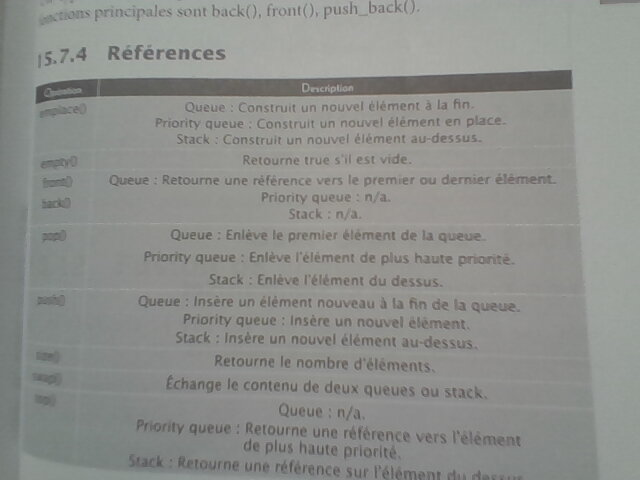
\includegraphics[width=2in]{stack_functions.png}
\end{center}

\section{Tries - Retrieval Trees - AutoComplete}

`std::queue` and `std::stack` containers as part of the standard library, but tries (retrieval trees) are not implemented. 

Here, and example with `std::unordered\_map` or `std::map` for the children nodes,
and custom classes or structs to represent the nodes.

Yet, third-party libraries have implementions of trie data structures.

\begin{verbatim}
#include <unordered_map>

class TrieNode {
public:
    bool isEndOfWord;
    std::unordered_map<char, TrieNode*> children;

    TrieNode() : isEndOfWord(false) {}
};

class Trie {
private:
    TrieNode* root;

public:
    Trie() {
        root = new TrieNode();
    }

    void insert(const std::string& word) {
        TrieNode* curr = root;
        for (char c : word) {
            if (curr->children.find(c) == curr->children.end()) {
                curr->children[c] = new TrieNode();
            }
            curr = curr->children[c];
        }
        curr->isEndOfWord = true;
    }

    bool search(const std::string& word) {
        TrieNode* curr = root;
        for (char c : word) {
            if (curr->children.find(c) == curr->children.end()) {
                return false;
            }
            curr = curr->children[c];
        }
        return curr->isEndOfWord;
    }
};

int main() {
    Trie trie;
    
    // Insert words into the trie
    trie.insert("apple");
    trie.insert("banana");
    trie.insert("cat");
    trie.insert("dog");
    
    // Search for words in the trie
    std::cout << trie.search("apple") << std::endl;  // Output: 1 (true)
    std::cout << trie.search("banana") << std::endl; // Output: 1 (true)
    std::cout << trie.search("cat") << std::endl;    // Output: 1 (true)
    std::cout << trie.search("dog") << std::endl;    // Output: 1 (true)
    std::cout << trie.search("car") << std::endl;    // Output: 0 (false)

    return 0;
}
\end{verbatim}

\subsection{Trie Serialization in JSON or XML}

To save a retrieval tree (trie) and use it later without recreating the tree every time,
you can serialize the tree data structure to a file and then deserialize it when needed.
This allows you to persist the tree structure to disk and load it back into memory when required.

Here are the general steps to achieve this:

1. Serialize the trie: Traverse the trie and convert its nodes and data
into a serialized representation that can be written to a file.
This typically involves converting the tree nodes and their contents into
a suitable format, such as JSON, XML, or a custom binary format.

2. Write the serialized data to a file:
Open a file in write mode and write the serialized data to the file.
You can use file I/O operations provided by the programming language or libraries to accomplish this.

3. Save the file: Close the file and make sure it is saved to a location of your choice,
such as a specific directory.

\textbf{Use the saved trie later}:

1. Read the serialized data from the file:
Open the saved file in read mode and read the serialized data from it.

2. Deserialize the data: Convert the serialized data back into the original trie data structure.
This involves parsing the serialized format and reconstructing the trie nodes and their relationships.

3. Use the trie: Once the trie is deserialized,
you can use it in your program for retrieval or any other operations as needed.

By saving and loading the serialized trie data,
you avoid the need to recreate the entire trie every time your program runs,
improving efficiency and performance.


\section{Trees}

\subsection{Breadth First Search}

\begin{verbatim}
#include <iostream>
#include <vector>
#include <queue>
#include <unordered_set>

using Graph = std::vector<std::vector<int>>;

// Breadth-First Search function
void bfs(const Graph& graph, int startNode) {
    int numNodes = graph.size();

    std::vector<bool> visited(numNodes, false);
    std::queue<int> q;

    q.push(startNode);
    visited[startNode] = true;

    while (!q.empty()) {
        int currentNode = q.front();
        q.pop();

        std::cout << currentNode << " ";

        for (int neighbor : graph[currentNode]) {
            if (!visited[neighbor]) {
                q.push(neighbor);
                visited[neighbor] = true;
            }
        }
    }
}

int main() {
    // Example graph represented as an adjacency list
    Graph graph = {
        {1, 2},      // Node 0 is connected to nodes 1 and 2
        {0, 2, 3},   // Node 1 is connected to nodes 0, 2, and 3
        {0, 1, 3},   // Node 2 is connected to nodes 0, 1, and 3
        {1, 2, 4},   // Node 3 is connected to nodes 1, 2, and 4
        {3, 5},      // Node 4 is connected to nodes 3 and 5
        {4}          // Node 5 is connected to node 4
    };

    int startNode = 0; // Starting node for BFS

    std::cout << "BFS traversal starting from node " << startNode << ": ";
    bfs(graph, startNode);
    std::cout << std::endl;

    return 0;
}
\end{verbatim}

\subsection{Depth First Search}

\begin{verbatim}
#include <iostream>
#include <vector>
#include <unordered_set>

using Graph = std::vector<std::vector<int>>;

// Depth-First Search function
void dfs(const Graph& graph, int currentNode, std::vector<bool>& visited) {
    std::cout << currentNode << " ";
    visited[currentNode] = true;

    for (int neighbor : graph[currentNode]) {
        if (!visited[neighbor]) {
            dfs(graph, neighbor, visited);
        }
    }
}

// Wrapper function for DFS to handle disconnected graphs
void dfsWrapper(const Graph& graph) {
    int numNodes = graph.size();
    std::vector<bool> visited(numNodes, false);

    for (int i = 0; i < numNodes; ++i) {
        if (!visited[i]) {
            dfs(graph, i, visited);
        }
    }
}

int main() {
    // Example graph represented as an adjacency list
    Graph graph = {
        {1, 2},      // Node 0 is connected to nodes 1 and 2
        {0, 2, 3},   // Node 1 is connected to nodes 0, 2, and 3
        {0, 1, 3},   // Node 2 is connected to nodes 0, 1, and 3
        {1, 2, 4},   // Node 3 is connected to nodes 1, 2, and 4
        {3, 5},      // Node 4 is connected to nodes 3 and 5
        {4}          // Node 5 is connected to node 4
    };

    std::cout << "DFS traversal: ";
    dfsWrapper(graph);
    std::cout << std::endl;

    return 0;
}
\end{verbatim}

\section{Graphs}

\chapter{Sorting Algorithms}


\section{Bubble Sort}

\section{Quick Sort}


\section{Adjacency Lists}

\subsection{Adjacency Matrix}




\section{Dijsktra Shortest Path}

Below is a C++ implementation of Dijkstra's algorithm for finding the shortest path in a weighted graph.
This implementation uses an adjacency list representation of the graph
and a priority queue (min heap) to efficiently select the next node with the smallest distance.


\begin{verbatim}
#include <iostream>
#include <vector>
#include <queue>
#include <limits>

const int INF = std::numeric_limits<int>::max();

// Node representation in the graph
struct Node {
    int index;
    int distance;

    Node(int idx, int dist) : index(idx), distance(dist) {}

    // Overload the comparison operator for the priority queue
    bool operator>(const Node& other) const {
        return distance > other.distance;
    }
};

// Dijkstra's algorithm for finding the shortest path
std::vector<int> dijkstraShortestPath(const std::vector<std::vector<std::pair<int, int>>>& graph, int source) {
    int n = graph.size();
    std::vector<int> distance(n, INF);
    distance[source] = 0;

    std::priority_queue<Node, std::vector<Node>, std::greater<Node>> pq;
    pq.push(Node(source, 0));

    while (!pq.empty()) {
        Node current = pq.top();
        pq.pop();

        if (current.distance > distance[current.index])
            continue;

        for (const auto& neighbor : graph[current.index]) {
            int newDistance = current.distance + neighbor.second;
            if (newDistance < distance[neighbor.first]) {
                distance[neighbor.first] = newDistance;
                pq.push(Node(neighbor.first, newDistance));
            }
        }
    }

    return distance;
}

int main() {
    int n = 5; // Number of nodes in the graph
    std::vector<std::vector<std::pair<int, int>>> graph(n);

    // Add edges to the graph (format: {destination, weight})
    graph[0].push_back({1, 5});
    graph[0].push_back({2, 3});
    graph[1].push_back({2, 2});
    graph[1].push_back({3, 6});
    graph[2].push_back({3, 7});
    graph[3].push_back({4, 4});

    int source = 0; // Source node

    std::vector<int> shortestDistances = dijkstraShortestPath(graph, source);

    // Print the shortest distances from the source node to all other nodes
    for (int i = 0; i < n; ++i) {
        std::cout << "Shortest dist from node " << source << " to node " << i;
        if (shortestDistances[i] == INF)
            std::cout << "Not reachable" << std::endl;
        else
            std::cout << shortestDistances[i] << std::endl;
    }

    return 0;
}
\end{verbatim}

\section{Algorithms}

\subsection{Accumulate}

\begin{verbatim}
// the algorithm everybody knows. (For_each and accumulate)

#include <numeric>

template<typename T>
T sum_data(const std::vector<T> &d) {
    return std::accumulate(d.begin(), d.end(), T());
}
\end{verbatim}

\subsection{Std::Puts}

Generating a null-terminated string,  a sequence of characters stored in an array
where the end of the string is marked by a null character ('\0'). 
The null character serves as a sentinel value to indicate the end of the string

\begin{verbatim}
#include <format>
#include <string_view>

void print_map(const auto &map, const std::string_view &key_desc = "key",
                                const std::string_view &value_desc = "value")
{
    for (const auto &[key, value] : map) /// structured binding
    {
        std::puts(std::format("{}: '{}' {}: '{}'",
                         key_desc, key, value_desc, value).c_str());

        // this is genious spacing for readability
    }
}

Standard c++20
\end{verbatim}
\subsection{Algorithms and Standard Template Library}

\begin{verbatim}
set<>
vector<>
for_each<>
any_of<>
etc.

A generic set of composable tools

// now, here we are

#include <numeric>
#include <vector>

template<typename Value_Type>
std::vector<Value_Type> get_data(const Value_Type &v1, const Value_type &v2,
                                 const Value_type &v3)
{
    std::vector<Value_Type> data;
    data.push_back(v1);
    data.push_back(v2);
    data.push_back(v3);
    return data;
}

template<typename T>
T sum_data(const std::vector<T> &d) {
    return std::accumulate(d.begin(), d.end(), T());
}

int main() {
    return sum)data(get_data(1,2,3));
}

// But we know the amount of data at compile-time. 
// If only there was some fixed-size container available!

\end{verbatim}

\subsection{Prefer Algorithms Over Loops}

Algorithms communicate meaning and help "const all the things".

Taking a functional approach and using algorithms, we can write cleaner c++.

\begin{verbatim}
// Algorithms end game (before C++20)

const auto has_value
    = std::any_of(begin(container), end(container), 
            greater_than(12));

// Algorithm end game (c++20)

const auto has_value
    = std::any_of(container, greater_than(12));

Next time you are reading through a loop in your codebase,
cross-reference it with the C++ <algorithm> header²
and try to find an algorithm that applies instead.

https://en.cppreference.com/w/cpp/algorithm
\end{verbatim}
\chapter{Cmake}

\section{Overview}

Cmake is super old. It has more than 300 functions to use, but 250 should not be used in modern cmake projects. 
This makes it particularly difficult to learn. Many older tutorials are confusing, out-of-date.

Moreover, modern cmake makes it as readable as possible with modern functions. Thus, way easier to read than older
functions.

\section{Compilers}

If your program has 3 .cpp files, the compiler would generate 3 object files. 
After all object files were compiled, the linker starts. 

\begin{center}
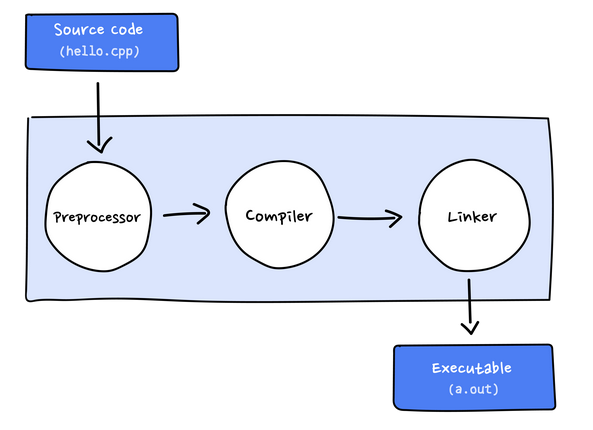
\includegraphics[width=3.5in]{compile.png}
\end{center}

\begin{center}
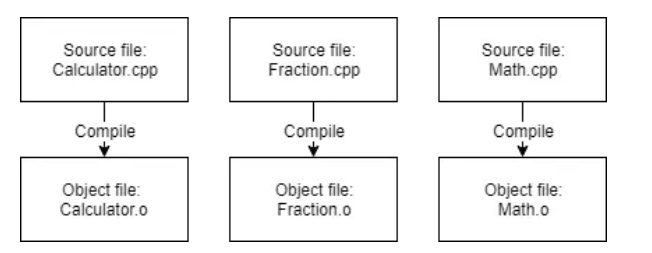
\includegraphics[width=3.5in]{compiling.png}
\end{center}

\begin{verbatim}
MVSC        // Microsoft Compiler
GCC         // Gnu C Compiler
LLVM Clang  // LLVM Compiler
\end{verbatim}

\subsection{Compile}
\begin{verbatim}
g++ hello.cpp -o hello

Compiling translates C++ programs into machine code.
It is stored on disk as a file with the .o extension (hello.o). 
\end{verbatim}

A linker then links the object code with standard library routines
that the program may use and creates an executable image which is also saved on disk,

usually as a file with the file name without any extension (e.g. hello).

\section{Linkers}

\begin{verbatim}
    It combined all object files in one executable.
    the linker links library files. 
    resolves cross-file dependencies.  
\end{verbatim}

\begin{center}
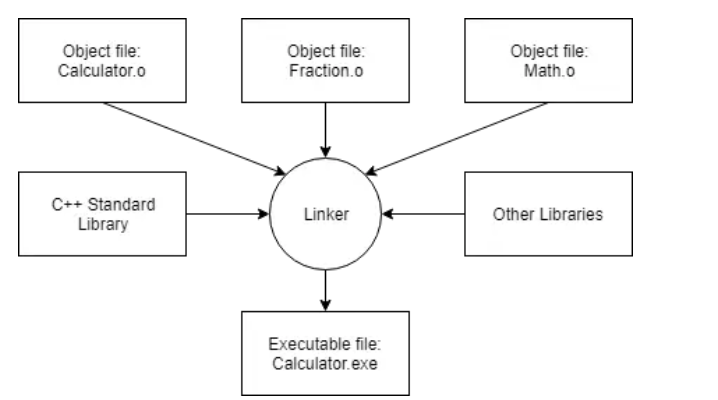
\includegraphics[width=4in]{linker.png}
\end{center}

\subsection{Link Header Files}

\begin{verbatim}
-- main.cpp --
#include "my_function.hpp"

$ g++ main.cpp my_function.cpp -o program

-- fun.hpp / fun.h --
double average(double num1, double num2);

-- fun.cpp --
double average(double num1, double num2) {
  return (num1 + num2) / 2;
}
\end{verbatim}

\subsection{Standard Library Headers}

\begin{verbatim}
Some standard library headers are included by others. 

<cstdlib> is included by <iostream>, since it relies on its functionalities,
such as the declaration of the system() function. 
\end{verbatim}

\section{Command Line Linking and Compiling}

\begin{verbatim}
g++ main.cpp my_functions.cpp // link both files
\end{verbatim}

\subsection{Source Code Files Suffix}

\begin{verbatim}
    .cpp (ex: hello.cpp) or
    .h (ex: std_lib_facilities.h).
\end{verbatim}


\section{Compiler Extensions (compiler-specific behavior)}


\textbf{This should not be in cmake, but in engineering}


Many compilers change the language through extentions. Non compliant c++ code is possible with them.
Extension are overpermissive and enabled by default.


Programs using non-standard extensions generally will not compile on other compilers 
(lacking same extensions support). If they do, they may not run correctly.

\begin{verbatim}
GCC
         -pedantic-errors // Disable extensions
\end{verbatim}

\section{Max Warnings}

\begin{verbatim}
GCC 
    -Wall -Weffc++ -Wextra -Wsign-conversion
    -Werror

Turner does it with cmake?
\end{verbatim}

\section{Standard Set-Up}

\begin{verbatim}
GCC pre-8
          -std=c++11 // set c++ standard
          -std=c++14
          -std=c++17
          -std=c++20 
GCC 8 or 9
          -std=c++2a for C++20 support

g++ -std=c++17 myfile.cpp -o output // cmd line
\end{verbatim}

\section{Precompiled Headers (PCH)}

Speed compilation in larger projects. A PCH file make subsequent compilations faster.




\section{Debugg and Error Type}

\subsection{Compile Time Errors}

\subsection{Synthax Errors}

\subsection{Type errors}

Forgetting to declare a variable

Storing a value in a different type. 

\subsection{Link-Time Errors}

link-time errors are based on unfindable needed function or library.

When the linker tries to combine object files into an executable.

\subsection{Run-Time Errors}

Errors which happen during program execution (run-time) after successful compilation.

Division by zero

Open an non-existing file

\subsection{Logical Errors}

Flawed programming's logical thinking. 

No errors, but output is wrong. 



\section{Project Structure}

See basic project and intermediate project examples, in cmake udemy.

\begin{center}
    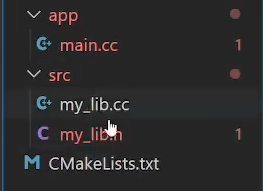
\includegraphics[width=2in]{cpp_tree1.png}
\end{center}


\begin{center}
    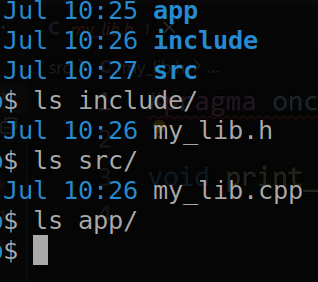
\includegraphics[width=2in]{cpp_tree2.png}
\end{center}

\subsection{App Directory}

Define everything important for the executable target, including its own CMakeLists.txt.

\subsection{Source Directory - src}

Define everything important for our library. When you have multiple libraries, create multiple directories in
src. As a naming convention, the subdirectory should have the same name as the library.

\begin{center}
    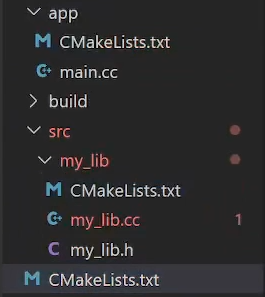
\includegraphics[width=2in]{cpp_tree3.png}
\end{center}

Don't forget to add a CMakeList in the src directory.


\begin{center}
    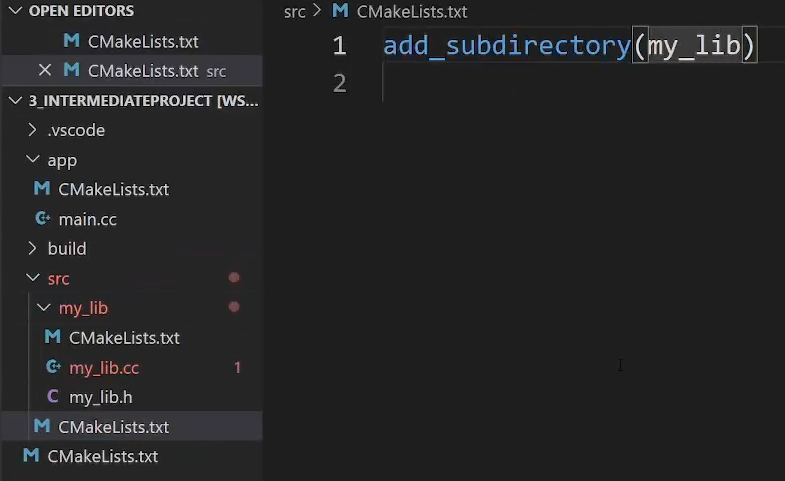
\includegraphics[width=4in]{cpp_tree4.png}
\end{center}

\subsection{CMake Default Paths}

Cmake has built-in paths to use. We use many in these notes.

\begin{verbatim}
# CMAKE_SOURCE_DIR is always the directory of the
# root CMakeLIsts.txt file
# our root directory

# CMAKE_BINARY_DIR is always our build directory
\end{verbatim}



\subsection{Template for Projects is Intermediate project}

Create a project builder based on the architecture of the intermediate project.


\section{Variables}

You can create variables for you executable or your libraries in the root CMakeLists.txt. The variables
will be usable in all add\_subdirectory chain at the end of the same document.

\begin{verbatim}
# set a variable for the library you want to use
# common synthax is capital letters.

# we reference Library in other CMakeLists files
# we change the Library name for LIBA

set(LIBA Library)

# where we used Library, write ${LIBA}


# we have used Hello for our executable name so far.
# we can change it as well.
set(HE Hello)

# where we used Hello, write ${HE}

add_subdirectory(src)
add_subdirectory(app)
\end{verbatim}


\subsection{Standard for cpp}

This is essential to have in your program. Otherwise, the compiler's default config will take the lead, with huge
variability between compiler versions!
In your root CMakeLists.txt file as well. This defines a variable and sets the standard to 17.

\begin{verbatim}
set(CMAKE_CXX_STANDARD 17)
set(CMAKE_C_STANDARD 98)
\end{verbatim}

\subsection{Standard Required}

Indicate that the compiler 100 pourcent implemented the language's standard.

\begin{verbatim}
set(CMAKE_CXX_STANDARD 17)
set(CMAKE_CXX_STANDARD_REQUIRED ON)
\end{verbatim}

\subsection{Compiler Extensions}

Some compilers have features that are not implemented in the Cpp standard. These features are extensions.
Some compilers allow you to use non-standard c code into a cpp program, even if they are not in the cpp standard.

\begin{verbatim}
set(CMAKE_CXX_STANDARD 17)
set(CMAKE_CXX_STANDARD_REQUIRED ON)
set(CMAKE_CXX_EXTENSIONS OFF)
\end{verbatim}

\subsection{If Statement}

Cmake has if statement. It even has string comparaison functions, to compare variable and create conditions.

\begin{verbatim}
option(COMPILE_EXECUTABLE "Whether to compile the executable" OFF)

add_subdirectory(src)

if (COMPILE_EXECUTABLE)
    add_subdirectory(app)
else()
    message("Without executable compiling")
endif()

\end{verbatim}


\subsection{Options}

You can set an option, the second argument is a simple comment for the reader (with no impact).

\begin{verbatim}
set(CMAKE_CXX_STANDARD 17)
set(CMAKE_CXX_STANDARD_REQUIRED ON)
set(CMAKE_CXX_EXTENSIONS OFF)

set(LIBA Library)
set(HE Hello)

option(COMPILE_EXECUTABLE "Whether to compile the executable" OFF)

add_subdirectory(src)

if (COMPILE_EXECUTABLE)
    add_subdirectory(app)
endif()


# to call the option from the command line

#$ cmake .. -DCOMPILE_EXECUTABLE=ON

# then you can switch it back OFF later

#$ cmake .. -DCOMPILE_EXECUTABLE=OFF
\end{verbatim}


\section{Makefile Shell Scripting}

Make is Cmake's ancestor. You can automate folder creation and files, just like any shell script would do. 

Make do not support space, use tabs.

\begin{verbatim}
prepare:
    rm -rf build
    mkdir build
    cd build

# to execute it

# $ make prepare
\end{verbatim}



\section{Project Software Toolkit}

\begin{verbatim}
Doxygen - create html documentation based on your codebase
Conan/VCPKG Packaging - How to install and use external libraries
Unit Testing
Code Coverage
CI Testing -- use all these tools in continuous integration, Github actions


We'll see how to create an html documentation based on your codebase
\end{verbatim}

\section{Installation Commands}

\begin{verbatim}
sudo apt-get update
sudo apt-get upgrade

# Mandatory
sudo apt-get install gcc g++ gdb
sudo apt-get install make cmake
sudo apt-get install git
sudo apt-get install doxygen
sudo apt-get install python3 python3-pip

# Optional
sudo apt-get install lcov gcovr
sudo apt-get install ccache
sudo apt-get install cppcheck
sudo apt-get install llvm clang-format clang-tidy
sudo apt-get install curl zip unzip tar

# for VSCODE

in extension, download franneck94 c/c++ extension pack
And the coding tools extension pack
Then, with command palette (in view), Config: generate C config file. It configures all tools the same as the
teacher's
\end{verbatim}

\section{Command Line Options}

\subsection{Generating a Project}

\begin{verbatim}
cmake [<options>] -S <path-to-source> -B <path-to-build>
\end{verbatim}

Assuming that a CMakeLists.txt is in the root directory, you can generate a project like the following.

\begin{verbatim}
mkdir build
cd build
cmake -S .. -B . # Option 1
cmake .. # Option 2

Assuming that you have already built the CMake project, you can update the generated project.

cd build
cmake .
\end{verbatim}

\subsection{Generator for GCC and Clang}

\begin{verbatim}
cd build
cmake -S .. -B . -G "Unix Makefiles" # Option 1
cmake .. -G "Unix Makefiles" # Option 2
\end{verbatim}

\subsection{Generator for MSVC}

\begin{verbatim}
cd build
cmake -S .. -B . -G "Visual Studio 16 2019" # Option 1
cmake .. -G "Visual Studio 16 2019" # Option 2
\end{verbatim}

\subsection{Specify the Build Type}

Per default, the standard type is in most cases the debug type.
If you want to generate the project, for example, in release mode you have to set the build type.

\begin{verbatim}
cd build
cmake -DCMAKE_BUILD_TYPE=Release ..
\end{verbatim}

\subsection{Passing Options}

If you have set some options in the CMakeLists, you can pass values in the command line.

\begin{verbatim}
cd build
cmake -DMY_OPTION=[ON|OFF] ..
\end{verbatim}

\subsection{Specify the Build Target (Option 1)}

The standard build command would build all created targets within the CMakeLists.
If you want to build a specific target, you can do so.

\begin{verbatim}
cd build
cmake --build . --target ExternalLibraries_Executable
\end{verbatim}

The target ExternalLibraries\_Executable is just an example of a possible target name.
Note: All dependent targets will be built beforehand.

\subsection{Specify the Build Target (Option 2)}


Besides setting the target within the cmake build command, you could also run the previously generated Makefile (from the generating step).
If you want to build the ExternalLibraries\_Executable, you could do the following.

\begin{verbatim}
cd build
make ExternalLibraries_Executable
\end{verbatim}


\section{Run the Executable}

After generating the project and building a specific target you might want to run the executable.
In the default case, the executable is stored in build/5\_ExternalLibraries/app/ExternalLibraries\_Executable, assuming that you are building the project 5\_ExternalLibraries and the main file of the executable is in the app dir.

\begin{verbatim}
cd build
./bin/ExternalLibraries_Executable
\end{verbatim}



\section{Configuration - Precompiling Information}

Create a configuration directory. With a config.hpp.in file.

\begin{center}
    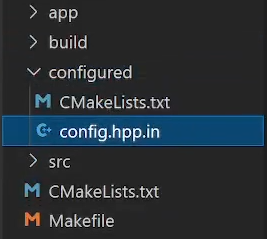
\includegraphics[width=2in]{conf.png}
\end{center}

In the CMakeLists.txt of this new configured directory.

\begin{verbatim}
configure_file(
    "config.hpp.in"
    # "${CMAKE_BINARY_DIR}" this is our build directory
                          # it is one of prebuilt directories in CMAKE
                          # thus, we reference it with CMAKE_BINARY_DIR
                          # we create an output for a config file, 
                          # in our build directory.

    # "${PROJECT_SOURCE_DIR}" # stores absolute path to project's root directory

    "${CMAKE_BINARY_DIR}/configured_files/include/config.hpp" ESCAPE_QUOTES)
\end{verbatim}

\subsection{Project Version Number}

In config.hpp.in

\begin{verbatim}
# @ cmake looks for and remplaces text between @@ this text @

#include <cstdint>
#include <string_view> 
static constexpr std::string_view project_name = "@PROJECT_NAME@";
static constexpr std::string_view project_version = "@PROJECT_VERSION@";
\end{verbatim}

\subsection{Sementic Versioning}

In version names: 1.0.0 . This is the first Major version (1). Incrementing the major version means
that the previous and the new codebase are not compatible at all. 2.0.0 have breaking changes with the 1.0.0 version.

The minor version 1.6.0, number 6 here, indicate that new features are available. Yet, nothing breaks between minor versions.

The patches are the last number, the last small fixes.

\begin{verbatim}
static constexpr std::int32_t project_version_major{@PROJECT_VERSION_MAJOR@};
static constexpr std::int32_t project_version_minor{@PROJECT_VERSION_MINOR@};
static constexpr std::int32_t project_version_patch{@PROJECT_VERSION_PATCH@};

#### Resulting file looks like.

#pragma once

#include <cstdint>
#include <string_view>

static constexpr std::string_view project_name = "CppProjectTemplate";
static constexpr std::string_view project_version = "1.0.0";

static constexpr std::int32_t project_version_major{1};
static constexpr std::int32_t project_version_minor{0};
static constexpr std::int32_t project_version_patch{0};
\end{verbatim}


\section{Sources and Headers}

When you have many libraries and many headers, create a variable for all of your headers.
Then, reference this variable to include everything.
List all of your source files in my\_lib directory.

\begin{verbatim}
set(LIBRARY_SOURCES
     "my_lib.cpp"
     "my_lib2.cpp"
     ) # quotes are not mandatory, just preference.
set(LIBRARY_HEADERS
     "my_lib.h")

add_library(${LIBRARY_NAME} STATIC
    "./"
    "${CMAKE_BINARY_DIR}/configured_files/include")
\end{verbatim}

\subsection{Executables}

You can do the same thing if you generate many executables, I think. This would be in your app directory.

\begin{verbatim}
set(EXE_SOURCES
    "main.cpp")

add_executable(${EXECUTABLE_NAME} ${EXE_SOURCES})
target_link_libraries(${EXECUTABLE_NAME} PUBLIC ${LIBRARY_NAME})
\end{verbatim}


\section{External Libraries}


\subsection{Git Submodule - nlohman json}

Create an external directory. Our project looks like this:

\begin{center}
    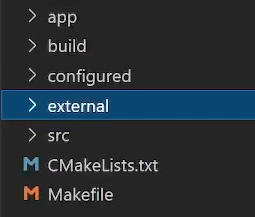
\includegraphics[width=2in]{external.png}
\end{center}

\begin{verbatim}
// make sure that your root folder is a git repo, git init

git submodule add https://github.com/nlogmann/json external/json

// it creates the json directory, when cloning the module in it.
\end{verbatim}

\subsection{Custom Cmake Functions}

In a cpp project, when you create your own cmake functions, they are stored in a Cmake directory. We just cloned a 
git repo in our external directory.

\begin{center}
    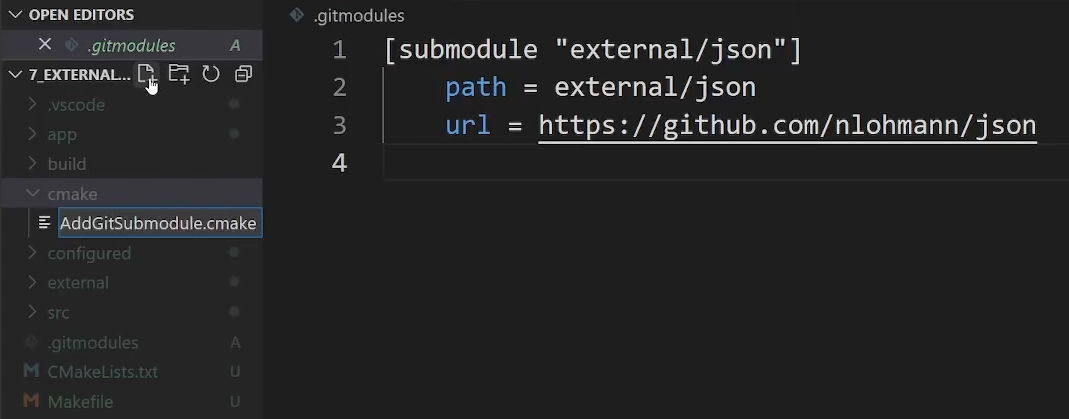
\includegraphics[width=4in]{add.png}
\end{center}

Now we create a AddGitSubmodule.cmake file. Inside, we define our function.

\begin{verbatim}
function(add_git_submodule dir) # our function takes one argument called dir
                                # this dir, is where the submodule is located
                                # making the add_ action possible.
        find_package(Git REQUIRED) # Git must be on your computer, or it
                                   # Error's out.
        if (NOT EXISTS ${dir}/CMakeLists.txt)
            execute_process (COMMAND ${GIT_EXECUTABLE}}
            submodule update --init --recursive -- ${dir}
                                                     # recursive is essential here
                                                     # If someone clones your project, 
                                                     # It automatically clones this submodules,
                                                     # It clones auto repos, inside your repo.
                                                            
            WORKING_DIRECTORY ${PROJECT_SOURCE_DIR}) # cmake saves some variable
                                                     # including the source dir
                                                     # of our project.
        endif()
        
        if (EXISTS ${dir}/CMakeLists.txt)
            message("Adding ${dir}/CMakeLists.txt")
            add_subdirectory(${dir})
        else
            message("Could not add ${dir}/CMakeLists.txt")
        endif()
endfunction(add_git_submodule)
\end{verbatim}


\subsection{Log example}

Here we are using an external library called log, with only two files, log.c and log.h . We have the library in our 
external directory. Plus, we have a CMakeLists.txt at the root of the external folder, taking care of the log library. 


\begin{center}
    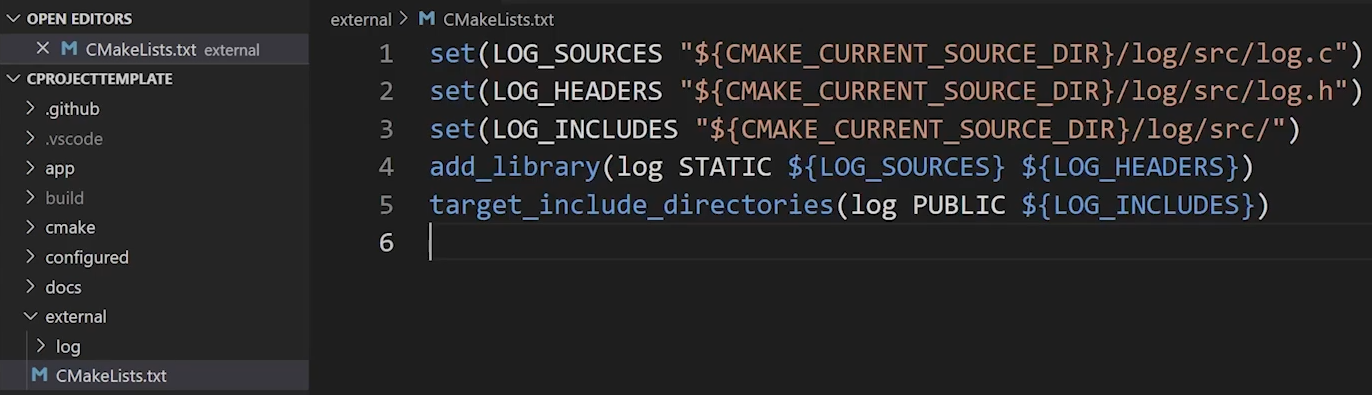
\includegraphics[width=5in]{loge.png}
\end{center}



\subsection{Call Your Own Functions}

In the source CMakeFiles.txt, knowing that we have a new git submodule. We add:


\begin{verbatim}
set(CMAKE_MODULE_PATH "${PROJECT_SOURCE_DIR}/cmake")
include(AddGitSubmodule) # includes indicates thats it a cmake module file.
                         # it will look where cmake modules are defined
                         # in our cmake dir


add_git_submodule(external/json) # this calls our custom function.

# In our app, we add this as well

set(EXE_SOURCES
    "main.cpp")

add_executable(${EXECUTABLE_NAME} ${EXE_SOURCES})
target_link_libraries(${EXECUTABLE_NAME} PUBLIC
    ${LIBRARY_NAME}
    nlohmann_json) # this links the submodule with the executable

# In main.cpp, we add 

#include <nlohman/json.hpp>
\end{verbatim}


\subsection{Fetch Content (fmt, spdlog, cxxopts, catch2)}

We have the gitmodule example, but modern CMake has a great fetching feature. Our root CMakelLists.txt will look like this, 

\begin{verbatim}
...

set(CMAKE_MODULE_PATH "${PROJECT_SOURCE_DIR}/cmake/")
include(AddGitSubmodule)


include(FetchContent)  # built-in library or file
                       # including it gives access to features

FetchContent_Declare() # Declare which github repository we would like to use
FetchContent_MakeAvailable() # will load this library in our cmake project.


                       # I want to use github.com/nlohmann/json
                       # any Gitlab is also possible
                       # I can do:
FetchContent_Declare(
    nlohmann_json      # since this repo is a cmake project,
                       # look at the project's root CMakeLists.txt file
                       # you will the name of the project, to enter here 
                       # see next image

    GIT_REPOSITORY https://github.com/nlohmann/json
    GIT_TAG v3.11.2    # the version I want to use
    GIT_SHALLOW TRUE)  # The function won't clone the repo recursively

                       # With this function, the git repository will be cloned in  
                       # our cloned repository.
                       # And it needs to be a cmake project.

                       # if it is not a cmake project, use the AddGitSubmodule method shown.
FetchContent_MakeAvailable(nlohmann_json) # will load this library in our cmake project.
\end{verbatim}

\begin{center}
    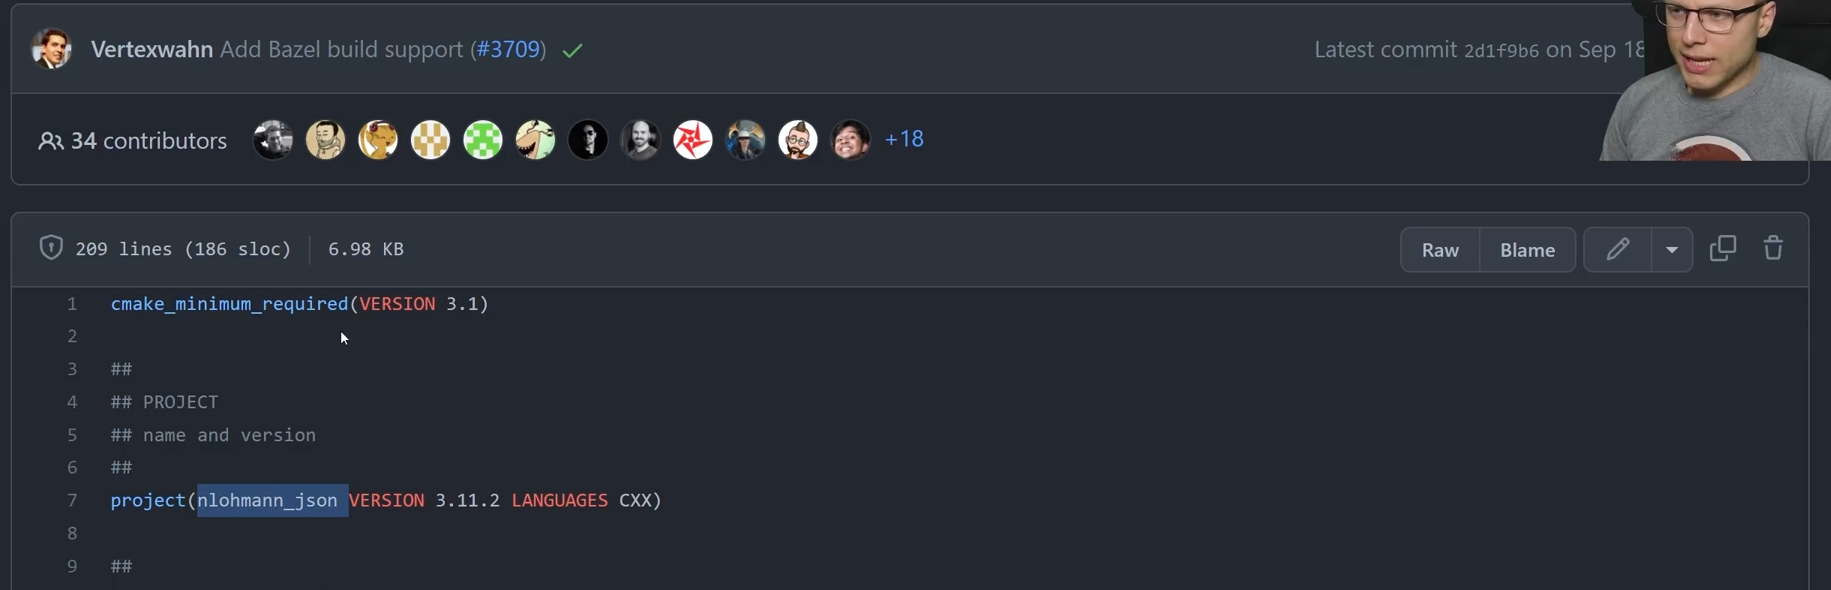
\includegraphics[width=5in]{json_n.png}
\end{center}


\subsubsection{FMT}

The best library to easily format strings in cpp.

\begin{verbatim}
FetchContent_Declare(
    fmt
    GIT_REPOSITORY https://github.com/fmtib/fmt
    GIT_TAG 9.1.0
    GIT_SHALLOW TRUE)
FetchContent_MakeAvailable(fmt)
\end{verbatim}

\subsubsection{spdlog}

The best fast logging library for cpp.

\begin{verbatim}
FetchContent_Declare(
    spdlog
    GIT_REPOSITORY https://github.com/gabime/spdlog
    GIT_TAG v1.11.0
    GIT_SHALLOW TRUE)
FetchContent_MakeAvailable(spdlog)
\end{verbatim}

\subsubsection{Cxxopts}

The best library to work with command line arguments in cpp. From the received arguments, to any other type.
The equivalent of the argument parser in python.

\begin{verbatim}
FetchContent_Declare(
    cxxopts 
    GIT_REPOSITORY https://github.com/jaroo2783/cxxopts
    GIT_TAG v3.0.0
    GIT_SHALLOW TRUE)
FetchContent_MakeAvailable(cxxopts)
\end{verbatim}

\subsubsection{Catch2}

The best Unit Testing library, seen further below.

\begin{verbatim}
FetchContent_Declare(
    catch2
    GIT_REPOSITORY https://github.com/catchorg/Catch2
    GIT_TAG v2.13.9  # teacher recommended this version, not the latest.
    GIT_SHALLOW TRUE)
FetchContent_MakeAvailable(catch2)
\end{verbatim}


\subsubsection{Include All Libraries in root CMakeListstxt}

Refer to Final project Template seen in the course. Modifying the CMakeLists.txt in our my-lib directory.

\begin{center}
    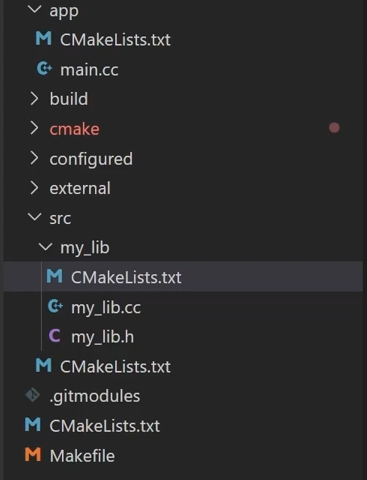
\includegraphics[width=2in]{final_p.png}
\end{center}

\begin{verbatim}
set(LIBRARY_SOURCES
    "my_lib.cpp")
set(LIBRARY_HEADERS
    "my_lib.h")
set(LIBRARY_INCLUDES
    "./"
    "${CMAKE_BINARY_DIR}/configured_files/include")

add_library(${LIBA} STATIC
    ${LIBRARY_SOURCES}
    ${LIBRARY_HEADERS})
target_include_directories(${LIBA} PUBLIC
    ${LIBRARY_INCLUDES})
target_link_libraries(${LIBA} PUBLIC
                                        # Naming convention is project_name::library_name
                                        # see next image, to find library_name in CMake project
                                        # on github
    
    nlohmann_json::nlohmann_json
    fmt::fmt
    spdlog::spdlog
    catch2::catch2
    cxxopts::cxxopts                    # not always the same

    )
\end{verbatim}

When this is set-up, and we reconfigure our cmake project, the repository will be cloned in a \_deps directory.
This includes a build, subbuild and src directory for all dependencies. Don't worry about it for now.

\begin{center}
    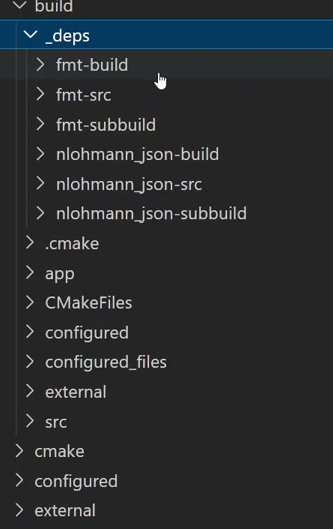
\includegraphics[width=2in]{deps.png}
\end{center}


\subsection{Include All Libraries in App Main.cpp}

It is tricky to include the libraries files in main. Some have directories, some do not.

\begin{verbatim}
#include <iostream>

#include <cxxopts.hpp>
#include <nlohman/json.hpp>
#include <fmt/format.h>
#include <spdlog/spdlog.h>
#include <catch2>

#include "my_lib.h"
#include "config.hpp"

int main() {
    ...
    std::cout << "CXXOPTS: # chose any included lib, to prove you have access to their info

    << CXXOPTS__VERSION_MAJOR << "."
    << CXXOPTS__VERSION_MINOR << "."
    << CXXOPTS__VERSION_PATCH << "." # if you have access to these variable, 
                                     # you have successfully imported and configure the lib
                                     # for you project.

    ...

}
\end{verbatim}


\subsection{Git Submodules vs Fetch Content}

If the repo is not a CMakeProject, you should use Git Submodules. Valid for GitHub and GitLab. In this case, 
define its own library target, I think. Not explained in detail.

If it is a CMake project on GitHub or Gitlab, use FetchContent. It is easier to use, you don't need to mess with header
libraries or anything. We can simply use the makeAvailable and prepare function.

The instructor highly recommends FetchContent!


\chapter{CMake Package Managers}

\section{CPM - Cmake Package Manager}

There are a few ways to include external libraries in you project. Git submodules, fetch content and packages managers such as
Cmake Package Manager.

On CPM's github page, click Releases. Pick the latest release, download the CPM.cmake file and copy it to your project's
cmake directory.

\begin{center}
    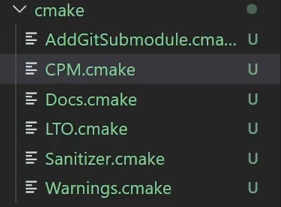
\includegraphics[width=2in]{cpm1.png}
\end{center}


\subsection{CPM Configuration in Root CMakeLists.txt}

Add an option in your root CMakeLists.txt.
Since the course's project has two different ways to import external libraries,
we will have an option for cpm and for fetch content.
We shouldn't use multiple tools at the same time. Thus, code
an if statement to use one or the other fetching method.

\textbf{Every external libraries used under CPM need to be github CMake projects, which 95 pourcent are.
It shouldn't be a problem}.


\textbf{Under the hood, CPM uses fetchcontent}. Therefore, the linking,
in the src/my\_lib/CMakeLists.txt file target\_link\_libraries function, 
can keep the fetchcontent synthax of nlohman\_json::nlohman\_json.


\begin{verbatim}
option(USE_CPM "Whether to use CPM" ON)

if(USE_CPM)
    message(STATUS "Using Cmake Package Manager")
    include(CPM)            # this includes the cpm.cmake file
    


                # "gh" cpm will look at github
                # "gh:nholmann" username
                # "gh:nholmann/json" repository name
                # "gh:nholmann/json#v3.11.2" version number 

    cpmaddpackage("gh:nholman/json#v3.11.2")    # This is CPM's defined function
    cpmaddpackage("gh:fmtlib/fmt#9.1.0")
    cpmaddpackage("gh:gabime/spdlog#v1.11.0")
    cpmaddpackage("gh:jarro2783/cxxopts#v3.1.1")
    cpmaddpackage("gh:cathorg/Catch2#v2.13.9")

else()
    message(STATUS "Using FetchContent")

    FetchContent_Declare(
        nlohmann_json      
        GIT_REPOSITORY https://github.com/nlohmann/json
        GIT_TAG v3.11.2    
        GIT_SHALLOW TRUE)  
    FetchContent_MakeAvailable(nlohmann_json) # will load this library in our cmake project.

    FetchContent_Declare(
        fmt
        GIT_REPOSITORY ...

endif()
\end{verbatim}

\section{Conan}

A package manager for cmake projects, alternatives to CPM and fetchcontent. CPM and fetchcontent localy
clones github repositories in your build directory. Then they compile the library locally, on your machine. 


Conan has a different approach. In an online database, pre-compiled repositories are available.
Conan downloads these. It depends on the compiler, but it generally saves compilation time.
No need to compile locally.

Conan binaries are compiled as release builds, not as debug builds.

A drawback for Conan is the binary updates. There are many configuration possible, and many updates
to keep track of. Therefore, many popular libraries won't have a compiled version for our machine's
configuration. Too many possibilities, Conan can't keep up with updates.

\subsection{Conan Installation}

\begin{verbatim}
Official installation guide is [here](https://docs.conan.io/2/).

The conan database is [here](https://conan.io/center/).

1. Install Python (3.7+)
2. Type ``pip install --user -U conan`` into the terminal
   1. Unix: Append conan to the PATH by: ``source ~/.profile``
3. Run: $ conan

4. $ conan profile detect --force
5. $ conan profile path default
\end{verbatim}


\subsection{Conan Configuration in Root CMakeLists.txt}

There is a pattern here, when you want to use something new in your cmake project,
set an option in the CMakeLists.txt file first.

Since the course shared examples for GitSubmodules, FetchContent, CPM and Conan,
we have a large if statement in our root CMakeLists.txt. In a regular project, 
select the tool you want, you wouldn't need the if.

\begin{verbatim}
option(USE_CONAN "Whether to use CPM" ON)

if(USE_CPM)
    ...
elseif(USE_CONAN)
    message(STATUS "Using Conan")
    include(${CMAKE_BINARY_DIR}/conan_toolchain.cmake  
                                # This is generated by a conan command
                                # in the conanfile.py (generate)
                                # including it in advance here.
    find_package(nlohmann_json REQUIRED)
    find_package(fmtlib REQUIRED)
    find_package(spdlog REQUIRED)
    find_package(cxxopts REQUIRED)
    find_package(Catch2 REQUIRED)

else()
    FetchContent_Declare(
        ...
\end{verbatim}

\subsection{Conanfile.py}

To configure conan, create a conanfile.py in your root directory.

\begin{center}
    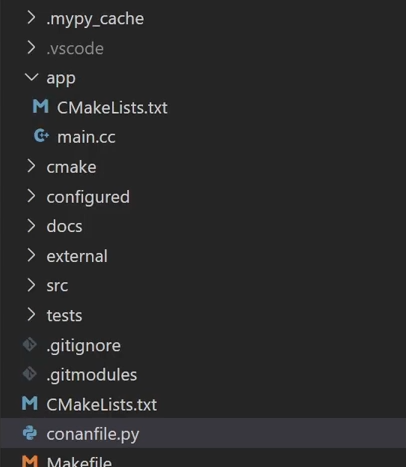
\includegraphics[width=2in]{conanfile.png}
\end{center}

\begin{verbatim}
from conan import ConanFile
from conan.tools.cmake import CMakeToolchain

class CompressorRecipe(ConanFile):
    settings = "os", "compiler", "build_type", "arch"
    generators = "CMakeDeps"

    def requirements(self):
        self.requires("nlohman_json/3.11.2")    # look at conan's database
                                                # to see which pre-compiled
                                                # versions are available
        self.requires("fmt/9.1.0")
        self.requires("spdlog/1.11.0")
        self.requires("catch2/2.13.9")
        self.requires("cxxopts/3.1.1")

    def generate(self):                         # this function generates the
                                                # conan_toolchain.cmake file
        tc = CMakeToolchain(self)
        tc.user_presets_path = False
        tc.generate()
\end{verbatim}

\subsection{Conan Debug Build}

Conan has release binaries by default, you have to tweak settings for you debug build.
To automatize conan's debug management, the instructor changed its makefile script.


\begin{verbatim}
conan_d:    # for conan debug
    rm -rf build
    mkdir build
    cd build && conan install .. -s build_type=Debug =s compiler.cppstd=17 --output-folder=. --build missing
                                -s               # for settings change
                                -- build missing 
                                                 # build binaries where no compiled version are available

conan_r:    # for conan release
    rm -rf build
    mkdir build
    cd build && conan install .. -s build_type=Release -s compiler.cppstd=17 --output-folder=. --build missing



### With this, run

$make conan_d
$make conan_r
\end{verbatim}  


\subsection{Conan Generated File}

Conan generates many files in your build directory, based on our configurations. Yet, no need to worry about them, conan
will deal with them.


\begin{center}
    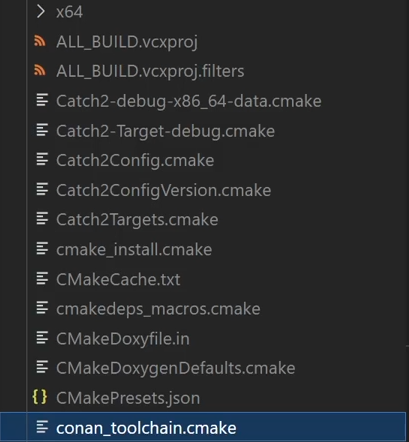
\includegraphics[width=2in]{conan2.png}
\end{center}

\section{VCPKG}

A C/C++ package manager for Microsoft. 
To use it, clone the VCPKG repository in your project's external library directory.

\begin{verbatim}
VCPKG database for available packages.

vcpkg.io/en/packages.html

Better is 

vcpkg.link 
\end{verbatim}

\subsection{VCPKG Installation}

Move to you project's external directory and clone the repo. Then, execute the .sh script.
 
\begin{verbatim}
Official Link: <https://vcpkg.io/en/index.html>

cd external
git clone https://github.com/Microsoft/vcpkg.git

.\vcpkg\bootstrap-vcpkg.bat  # windows
./vcpkg/bootstrap-vcpkg.sh   # Unix

cd vcpkg 
vcpkg --help 
\end{verbatim}


\subsection{VCPKG.json file in project root}

List dependencies of your cmake project in a JSON file. VCPKG's synthax is very tricky, plus its 
requirements are complicated for no reason.

It automatically downloads the latest versions of all libraries. Thus, if we want one particular
version, we need this overrides keyword.

\begin{verbatim}
{
    "name": "cpptemplateproject",
    "version-string": "1.0.0",
    "dependencies": [
        {
            "name": "cxxopts",
            "version>=": "3.1.1"
        },
        {
            "name": "fmt",
            "version>=": "9.1.0"
        },
        {
            "name": "nlohmann-json",
            "version>=": "3.11.2"
        },
        {
            "name": "spdlog",
            "version>=": "1.11.0"
        },
        {
            "name": "catch2",
            "version>=": "2.13.9"
        }
    ],
    "overrides": [
        {
            "name": "catch2",
            "version": "2.13.9"
        }
    ],
    "builtin-baseline": "40619a55c3e76dc4005c8d1b7395071471bb8b96"

    # this baseline is the hexadecimal value
    # of a certain VCPKG git commit

    # this is ridiculously complicated,
    # in this examples here, we git logged the external/vcpkg directory of our project.
}
\end{verbatim}


\begin{center}
    
\includegraphics[width=2in]{ridiculous.png}
\end{center}


After configuration, libraries are downloaded and compiled on your system.


\begin{center}
    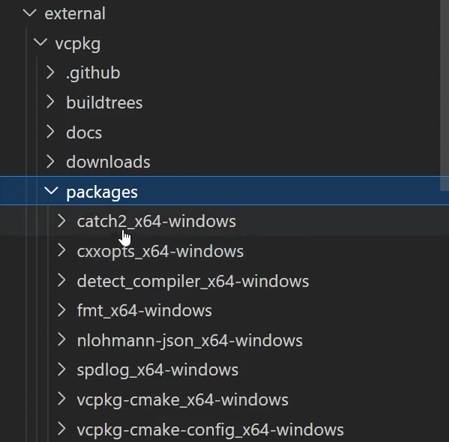
\includegraphics[width=2in]{vcpkg2.png}
\end{center}


\subsection{VCPKG configuration in root CMakeLists.txt}

Include vcpkg.cmake file in our project.

\begin{verbatim}
option(USE_CONAN "Whether to use CPM" ON)

if(USE_CPM)
    ...
elseif(USE_CONAN)
    message(STATUS "Using Conan")
    include(${CMAKE_BINARY_DIR}/conan_toolchain.cmake  
                                # This is generated by a conan command
elseif(USE_VCPKG)
    message(STATUD "Using VCPKG")

    include(${CMAKE_SOURCE_DIR}/external/vcpkg/scripts/buildsystems/vcpkg.cmake)
    find_package(nlohmann_json REQUIRED)
    find_package(fmt REQUIRED)
    find_package(..  REQUIRED)

else()
    FetchContent_Declare(
        ...
\end{verbatim}

\section{Package Managers Summary}

There are many ways to add and include libraries to our cmake project: Git Submodules, FetchContent,
Cmake Package Manager (CPM), Conan and VCPKG.

Use Git Submodules if you github repo you want to use is not a cmake project. It is a rare case, but it is
the best solution. Do not use this approach if they are cmake projects.


\textbf{CPM is the instructors' recommendation} for all gitlab and github cmake projects. However, it is important to understand the FetchContent functions of 
CMake. CPM uses these same fetch content methods under the hood.


VCPKG is hard to configure and version download complications. Not recommended.

Conan's pre-built binaries are a great idea, but they do not update these binaries often enough. 
However, if you have huge libraries that take 30 minutes to compile. Conan is the way to go.

\chapter{CMake Tooling}

\section{Dependency Graphs}

In a makefile, or any script, use the command --graphviz. Dependency and prepare are the flag needed to run the command.

\begin{verbatim}
dependency:
    cd build && cmake .. --graphviz=grap.dot && dot -Tpng graph.dot -o grapImage.png
                        // not yet an image when .dot
                        // but easy to transform
prepare:
    rm -rf build
    mkdir build
                        // unrelated to dependency graph.
\end{verbatim}

The house symbol is the executable. Rectangle are external libraries. Losanges shapes are internal libraries.

\begin{center}
    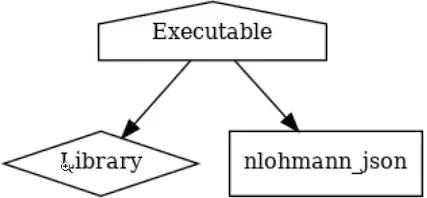
\includegraphics[width=2in]{graph.png}
\end{center}

Towards the end of the course, the graph was more complex.

\begin{center}
    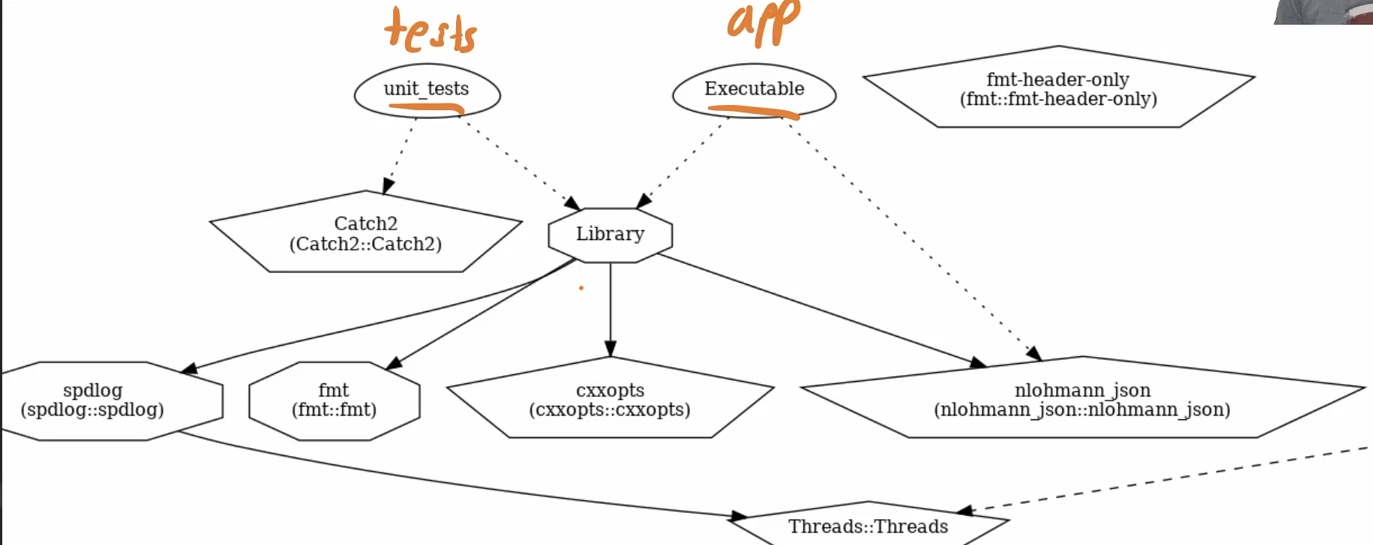
\includegraphics[width=5in]{graph3.png}
\end{center}

\section{Doxygen Documentation}

Generate html documentation for our code. For example, for our library. The course has a vscode extention: Doxygen Documentation Generator.

\subsection{Doxygen Vscode Extension}

The extention generates documentation base on this synthax.

\begin{verbatim}
#include <iostream>

#include <nlohmann/json.hpp>
#include "my_lib.h"

/**
 * @brief Prints out hello world and tests the JSON lib.
 *
 *
 */
\end{verbatim}

\subsection{Doxygen Command Line}

Doxygen is looking for a doxy file, a config file. Generate a doxy file with doxygen -g.
In it, fill information on the project, name, version,  path to source files, etc. It will generate better html file with the information.
In the docs directory.

\begin{center}
    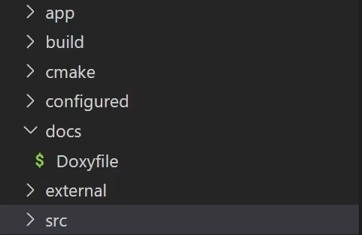
\includegraphics[width=2in]{dox.png}
\end{center}

\begin{verbatim}
# Configuration for Doxygen for use with CMake
# Only options that deviate from the default are included
# To create a new Doxyfile containing all available options, call `doxygen -g`

#---------------------------------------------------------------------------
# Project related configuration options
#---------------------------------------------------------------------------
DOXYFILE_ENCODING       = UTF-8
PROJECT_NAME            = "C++ Project Template"
PROJECT_NUMBER          = 1.0
PROJECT_BRIEF           =
PROJECT_LOGO            =
OUTPUT_DIRECTORY        = ./
OUTPUT_LANGUAGE         = English
MARKDOWN_SUPPORT        = YES

#---------------------------------------------------------------------------
# Build related configuration options
#---------------------------------------------------------------------------
EXTRACT_ALL             = YES
RECURSIVE               = YES
GENERATE_HTML           = YES
GENERATE_LATEX          = NO

#---------------------------------------------------------------------------
# Configuration options related to the input files
#---------------------------------------------------------------------------
INPUT                  =    ../src \
INPUT                       ../include
INPUT_ENCODING         = UTF-8
FILE_PATTERNS          = *.c \
                         *.cc \
                         *.cpp \
                         *.c++ \
                         *.h \
                         *.hpp \
                         *.h++ \
                         *.md \
                         *.dox \
                         *.doc \
                         *.txt
\end{verbatim}

When ready, generate the html with the command Doxygen, inside the docs folder (where the doxyfile is located). It creates an html dir.
it has the index.html automatically. The webpage looks like this:


\begin{center}
    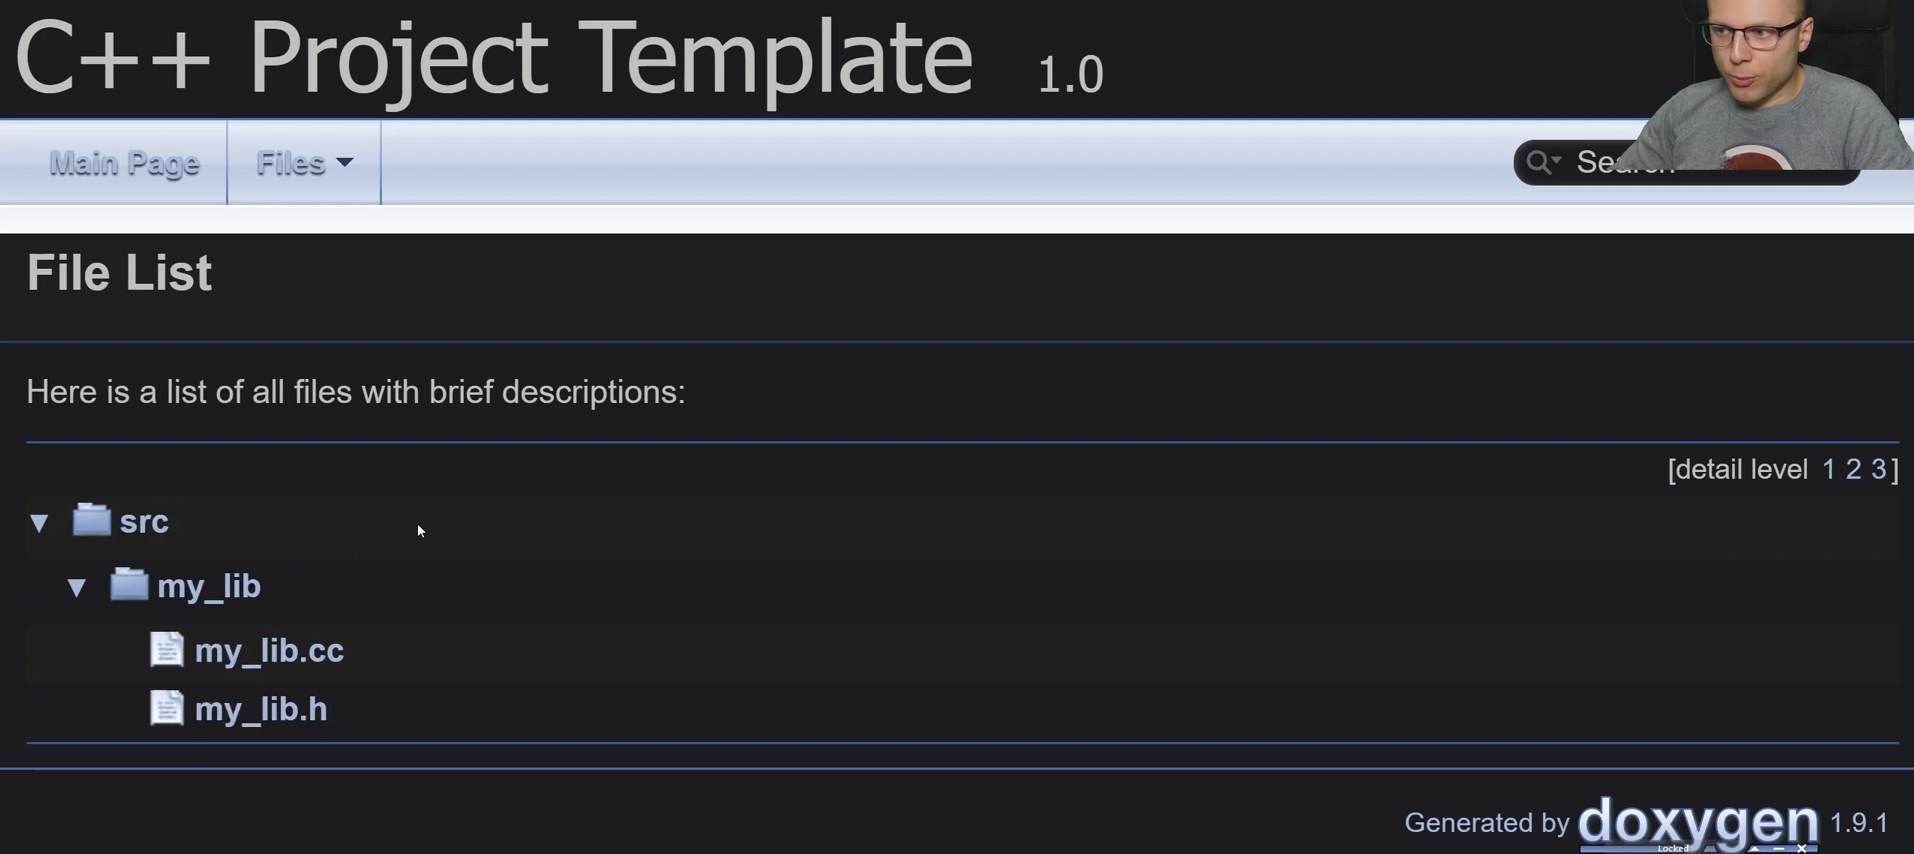
\includegraphics[width=5in]{dox2.png}
\end{center}


\subsection{Doxygen Custom Target Documentation}

We need to add the documentation to our cmake project.

\begin{center}
    
\includegraphics[width=3in]{doccmake.png}
\end{center}

In our root CMakeLists.txt, we add.

\begin{verbatim}
include(AddGitSubmodule)
include(FetchContent)
include(Docs)               # this is our new dir.

\end{verbatim}


\subsection{Doxygen Doc.cmake}

Cmake needs to find Doxygen, because we are using it for our docs. In Docs.cmake,

\begin{verbatim}
find_package(Doxygen)
if (DOXYGEN_FOUND)
    add_custom_target( # This is just an utility target
                       # With it, we can interact with it, 
                       # in the terminal
    docs
    ${DOXYGEN_EXECUTABLE}
    WORKING_DIRECTORY ${CMAKE_SOURCE_DIR}/docs

                       # CMAKE_SOURCE_DIR is always the directory of the
                       # root CMakeLIsts.txt file
                       # our root directory

                       # CMAKE_BINARY_DIR is always our build directory
endif()
\end{verbatim}

Now Documentation can be built seperately, independently of the main project app built process.

\section{Catch2 - Unit Testing}

\subsection{Function Unit Testing}

Adding Unit test to our codebase, with the catch2 library. Unit tests are useful to test functions from the library.

There is a tutorial on the github catch2 page. As an example, it provides this factorial function example, to try.

\begin{verbatim}
unsigned int factorial( unsigned int number ) {
    return number <= 1 ? number : factorial(number-1)*number;
}

// the instructor changes it to

std::uint32_t factorial(std::unint32_t number)
{

    return number <= 1 ? number : factorial(number-1) * number;

}
\end{verbatim}


\subsection{Unit Test Directory}

To introduce unit testing, we create a new directory: tests.

\begin{center}
    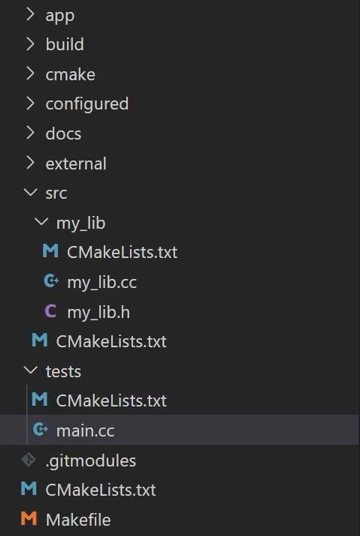
\includegraphics[width=2in]{tests.png}
\end{center}

In our root CMakeLists.txt.  

\begin{verbatim}
add_subdirectory(configured)
add_subdirectory(external)
add_subdirectory(src)
add_subdirectory(app)
add_subdirectory(tests) # adding tests
\end{verbatim}

\textbf{The idea is to have our main executable, our library(lib) and our unit test executable. The main and the Unit
executable we'll both use our library, but we will test with Unit. Unit will test if all our implemented functions work without bugs.}


\subsection{Unit Tests Configuration CMakeLists.txt}

\begin{verbatim}
set(TEST_MAIN "unit_tests")        # this is the name of our testing executable
set(TEST_SOURCES "main.cpp")       # Here, the tests are in one file only
                                   # It could be divided into more files
                                   # Header files for example
set(TEST_INCLUDES "./")
add_executable(${TEST_MAIN} ${TEST_SOURCES})
target_include_directories(${TEST_MAIN} PUBLIC ${TEST_INCLUDES})
target_link_libraries(${TEST_MAIN} PUBLIC ${LIBA} Catch2::Catch2)

                                   # Our library is linked, LIBA
                                   # This is how we will test it
\end{verbatim}


\subsection{Unit Tests Definition}

To test the factorial function, this is the test definition given as example.

\begin{verbatim}
#define CATCH_CONFIG_MAIN // This tells Catch to provide a main() - only do this in one file
                          // No need to write int main() {}, this does it. 
#include "catch2/catch.hpp"

#include "my_lib.h"       // Will be called in my_lib.h

TEST_CASE( "Factorials are computed", "[factorial]" ) {
    REQUIRE( Factorial(1) == 1);
    REQUIRE( Factorial(2) == 2);
    REQUIRE( Factorial(3 == 6);
    REQUIRE( Factorial(10 == 362880 );
}

This function needs to be called in my_lib.h

std::uint32_t factorial(std::uint32_t number);
\end{verbatim}


\subsection{Unit Testing Command Line Options}

It is convenient to have a command line option to activate or deactivate our testing build. In our root CMakeLists.txt
file, we add an option. In our CMakeLists.txt in the tests directory, we add an if statement. 

\begin{verbatim}
option(ENABLE_TESTING "Enable a Unit Testing Build" ON) 

# in tests directory's CMakeLists.txt

if (ENABLE_TESTING)
    set(TEST_MAIN "unit_tests")
    set(TEST_SOURCES "main.cpp")
    set(TEST_INCLUDES "./")

    add_executable(#{TEST_MAIN} ${TEST_SOURCES})
    target_include_directories(${TEST_MAIN} PUBLIC ${TEST_INCLUDES})
    target_link_libraries(${TEST_MAIN} PUBLIC ${LIBA} Catch2::Catch2)
endfi()
\end{verbatim}


\subsection{On Testing Libraries in General}

The specific words (Test\_case, require, etc.) may vary a bit, but they all have the same logic. When you are familiar with one, 
you will be able to use another testing library.

\begin{verbatim}
You have a test case, 

TEST_CASE()

You can give it a name and a short-name(abbriviated)

TEST_CASE( "Factorials are computed", "[factorial]" )

you can test a function with a keyword like require, or require_equal. Giving an input, the result should be. 
REQUIRE( factorial(0) == 0)
\end{verbatim}

\section{Linking Types Differences} 

Public and private is similar to OOP public and private keywords in classes.

\begin{verbatim}
add_library(A ...)
add_library(B ...)
add_library(C ...)
\end{verbatim}

\subsection{Linking Type Public}

Here, fmt can be used in the library of A. 

\begin{verbatim}
target_link_libraries(A PUBLIC fmt)

target_link_libraries(C PUBLIC/PRIVATE A)
target_link_libraries(C PUBLIC/PRIVATE A)
\end{verbatim}

When A links fmt as PUBLIC, it says that A uses fmt in its implementation, and fmt is also used in A's public API.
Hence, C can use fmt since it is part of the public API of A.

\subsection{Linking Type Private}

Using PRIVATE does not make the library available in the target's public API. Instead, it is part of a private API.
When B links in spdlog as PRIVATE, it is saying that B uses spdlog in its implementation,
but spdlog is not used in any part of B's public API. 

\begin{verbatim}
target_link_libraries(B PRIVATE spdlog)

target_link_libraries(C PUBLIC/PRIVATE B)
\end{verbatim}

Any code that makes calls into B would not need to refer directly to anything from
spdlog.


In a professional setting, you want to keep certain aspect of you project private. Hence, this option to consider.

\subsection{Linking Type Interface}

In general, used for header-only libraries. That is, libraries where you don't need to compile anything. They do not have
any compilation logic in them.

\begin{verbatim}
add_library(D INTERFACE)
target_include_directories(D INTERFACE {CMAKE_CURRENT_SOURCE_DIR}/include)

# this only links something to the executable, I think. No compilation logic.
\end{verbatim}


\section{Library Types Difference}

\subsection{Library Type Library}

A binary file that contains information about code.
A library cannot be executed on its own.
An application utilizes a library.

A library must be build too, if it is used by an executable.

\begin{verbatim}
cmake --build . --target Library
cmake --build . --target Executable // it is dependent to the Library build!
\end{verbatim}

\subsection{Library Type Shared}

\begin{verbatim}
Linux: *.so
MacOS: *.dylib
Windows: *.dll
\end{verbatim}

Shared libraries reduce the amount of code that is duplicated in each program that makes use of the library, keeping the binaries small.
Shared libraries will however have a small additional cost for the execution.
In general the shared library is in the same directory as the executable.

A file that needs to be carried along with the executable.

\begin{center}
    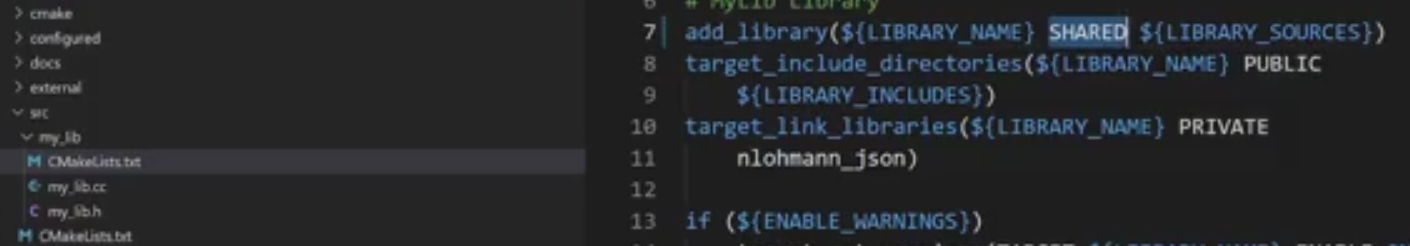
\includegraphics[width=2in]{shar.png}
\end{center}


\subsection{Library Type Static}

\begin{verbatim}
Linux/MacOS: *.a
Windows: *.lib
\end{verbatim}

Static libraries increase the overall size of the binary, but it means that you don't need to carry along a copy of the library that is being used.
As the code is connected at compile time there are not any additional run-time loading costs.

A staticly compiled into the executable.


\section{Compiler Warnings}

You can pull certain warnings for a particular target.
We can activate them based on the operating system and on the compiler.
We can trigger certain set of compiler checks.
In this course, we had two targets: the library target and the executable target.

In the cmake directory, add Warnings.cmake. 

\begin{center}
    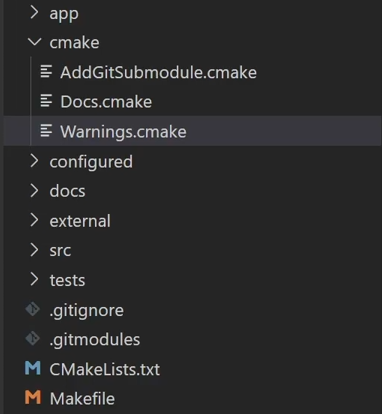
\includegraphics[width=2in]{warnings1.png}
\end{center}

\begin{verbatim}
function(target_set_warnings)
    set(oneValueArgs TARGET ENABLE AS_ERRORS)
    cmake_parse_arguments(
        TARGET_SET_WARNINGS             # every option and oneValueArgs
                                        # will be prefixed by
                                        # TARGET_SET_WARNINGS


                                        # this function was updated at the end of the course.
                                        # refactoring at the end of the course was hard to follow.
        "${options}"
        "${oneValueArgs}"
        "${multiValueArgs}"
        ${ARGN})

    if (NOT ${TARGET_SET_WARNINGS_ENABLE})
        message(STATUS "Warnings disabled for: ${TARGET_SET_WARNINGS_TARGET}")
        return()
    endif()
    message(STATUS "Warnings Active for: ${TARGET_SET_WARNINGS_TARGET}")
    message(STATUS "Warnings as Errors: ${TARGET_SET_WARNINGS_AS_ERRORS}")

    set(MSCV_COMPILER
        /WA4
        /permissive-)

    set(CLANG_COMPILER
        -Wall
        -Wextra
        -Wpedantic)

    set(GCC_WARNINGS ${CLANG_WARNINGS})

    if(${ENABLED_AS_ERRORS}}
        set(MSCV_WARNINGS ${MSVC_WARNINGS} /WX) # We need to append to our MSVC compiler
                                                # We append /WX

        set(CLANG_WARNINGS ${CLANG_WARNINGS} -Werror)
                                                # We append -Werror
        set(GCC_WARNINGS ${GCC_WARNINGS} -Werror)
    endif()

    if(CMAKE_CXX_COMPILER_ID MATCHES "MSVC")
        set(WARNINGS ${MSVC_WARNINGS})
    elseif(CMAKE_CXX_COMPILER_ID MATCHES "CLANG")
        set(WARNINGS ${CLANG_WARNINGS})
    elseif(CMAKE_CXX_COMPILER_ID MATCHES "GNU")
        set(WARNINGS ${GCC_WARNINGS})
    endif()

    target_compile_options(${TARGET} PRIVATE ${WARNINGS})
    message(STATUS ${WARNINGS})

endfunction(target_set_warnings TARGET)
\end{verbatim}

\subsection{Compiler Check User's Compiler}

\begin{verbatim}
if(CMAKE_CXX_COMPILER_ID MATCHES "MSVC")
    set(WARNINGS ${MSVC_WARNINGS})
elseif(CMAKE_CXX_COMPILER_ID MATCHES "CLANG")
    set(WARNINGS ${CLANG_WARNINGS})
elseif(CMAKE_CXX_COMPILER_ID MATCHES "GNU")
    set(WARNINGS ${GCC_WARNINGS})
endif()
\end{verbatim}


\subsection{Compiler Warnings Root CMakeLists Options}

We just created a function to check the user's compiler and set compilation warnings.
Now create options in the root CMakeFilelists.txt.

\begin{verbatim}
option(ENABLE_WARNINGS "Enable warnings" ON)
option(ENABLE_WARNINGS_AS_ERRORS "Enable warnings as errors" ON)

    ...

if(ENABLE_WARNINGS)
    include(Warnings) # include the newly created Warnings.cmake file
endif()
\end{verbatim}


\subsection{Compiler Warnings Executable Target}

There are two targets that can have compilation warnings, our library and our executable (our app). We have to 
add warning conditionals in both of their CMakeLists.txt file.

\begin{verbatim}
if(${ENABLE_WARNINGS})
    target_set_warnings(
        ${HE}       # this is our executable / app name,
                    # passed as argument in our created warnings function
        ${ENABLE_WARNINGS}
        ${ENABLE_WARNINGS_AS_ERRORS})
endif()

# for the lib CMakeLists.txt

if(${ENABLE_WARNINGS})
    target_set_warnings(
        ${LIBA}       # this is our library target name,
                      # passed as argument in our created warnings function
        ${ENABLE_WARNINGS}
        ${ENABLE_WARNINGS_AS_ERRORS})
endif()
\end{verbatim}

You don't have to have warnings as error for all targets, but you should have compilation warnings for all of them.

\section{Sanitizers}

Use sanitizers to find memory links or memory problems in your code. Sanitizers are used at runtime. 
Thus, it happens after compilation. Clang-tidy is a static linter, it finds problems before compilation!  

In order, you have clang-tidy before compilation, 
compiler warnings during compilation and sanitizers at runtime (after compilation).

In our root CMakeLists.txt, we add

\begin{verbatim}
option(ENABLE_SANITIZE_ADDR "Enable warnings" ON)
option(ENABLE_SANITIZE_UNDEF "Enable warnings" ON)


if(ENABLE_SANITIZE_UNDUF OR ENABLE_SANITIZE_ADDR)
    include(Sanitizers) # include a Sanitizers.cmake file
                        # same as Warnings.cmake file
endif()

\end{verbatim}

\begin{center}
    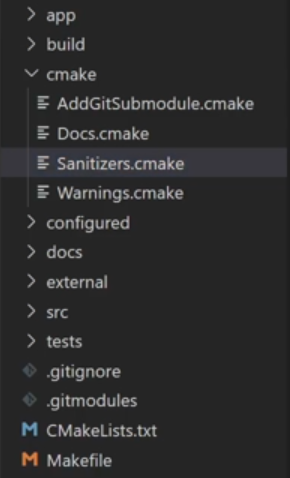
\includegraphics[width=2in]{san.png}
\end{center}


\subsection{Sanitizers.cmake}

In cmake directory, we have this file.


\begin{verbatim}
function(add_sanitizer_flags)
    if(NOT ${ENABLE_SANITIZE_UNDEF} AND NOT ${ENABLE_SANITIZE_ADDR})
        message(STATUS "Sanitizers deactivated") 
        return()
    endif()

    if(CMAKE_CXX_COMPILER_ID MATCHES "CLANG" OR CMAKE_CXX_COMPILER_ID MATCHES "GNU")
        add_compile_options("-fno-omit-frame-pointer")   
                                        # This functions adds compiler flags for every target
                                        # Sanitizers need to run on all of the application
        add_link_options("-fno-omit-frame-pointer")

        if (${ENABLE_SANITIZE_ADDR})
            add_compile_options("-fsanitize=address") 
            add_link_options("-fsanitize=address") 
        endif()

        if (${ENABLE_SANITIZE_UNDEF})
            add_compile_options("-fsanitize=undefined") 
            add_link_options("-fsanitize=undefined") 
        endif()

    elseif(CMAKE_CXX_COMPILER_ID MATCHES "MSVC")
        if (${ENABLE_SANITIZE_ADDR})
            add_compile_options("-fsanitize=address") 
            add_link_options("-fsanitize=address") 
        endif()

        if (${ENABLE_SANITIZE_UNDEF})
            message(STATUS "Undefined sanitizer is not implemented for MVSC")
        endif()

    else() 
        message(ERROR "Compiler not supported for Sanitizers")
    endif()
endfunction()
\end{verbatim}


\subsection{Sanitizers Activation in Root CMakeLists.txt}

Call the add\_sanitizer\_flags function from root.

\begin{verbatim}
if(ENABLE_SANITIZE_ADDR OR ENABLE_SANITIZE_UNDEF)
    include(Sanitizers)
    add_sanitizer_flags()
endif()
\end{verbatim}

\subsection{Sanitizer Bugs}

Going out of bounds, like this, would be caught be clang-tidy, but not by compilers. Thus, Sanitizers help big time. See documentation at
gcc.gnu.org/onlinedocs/Instrumentation-Options.html.


\begin{center}
    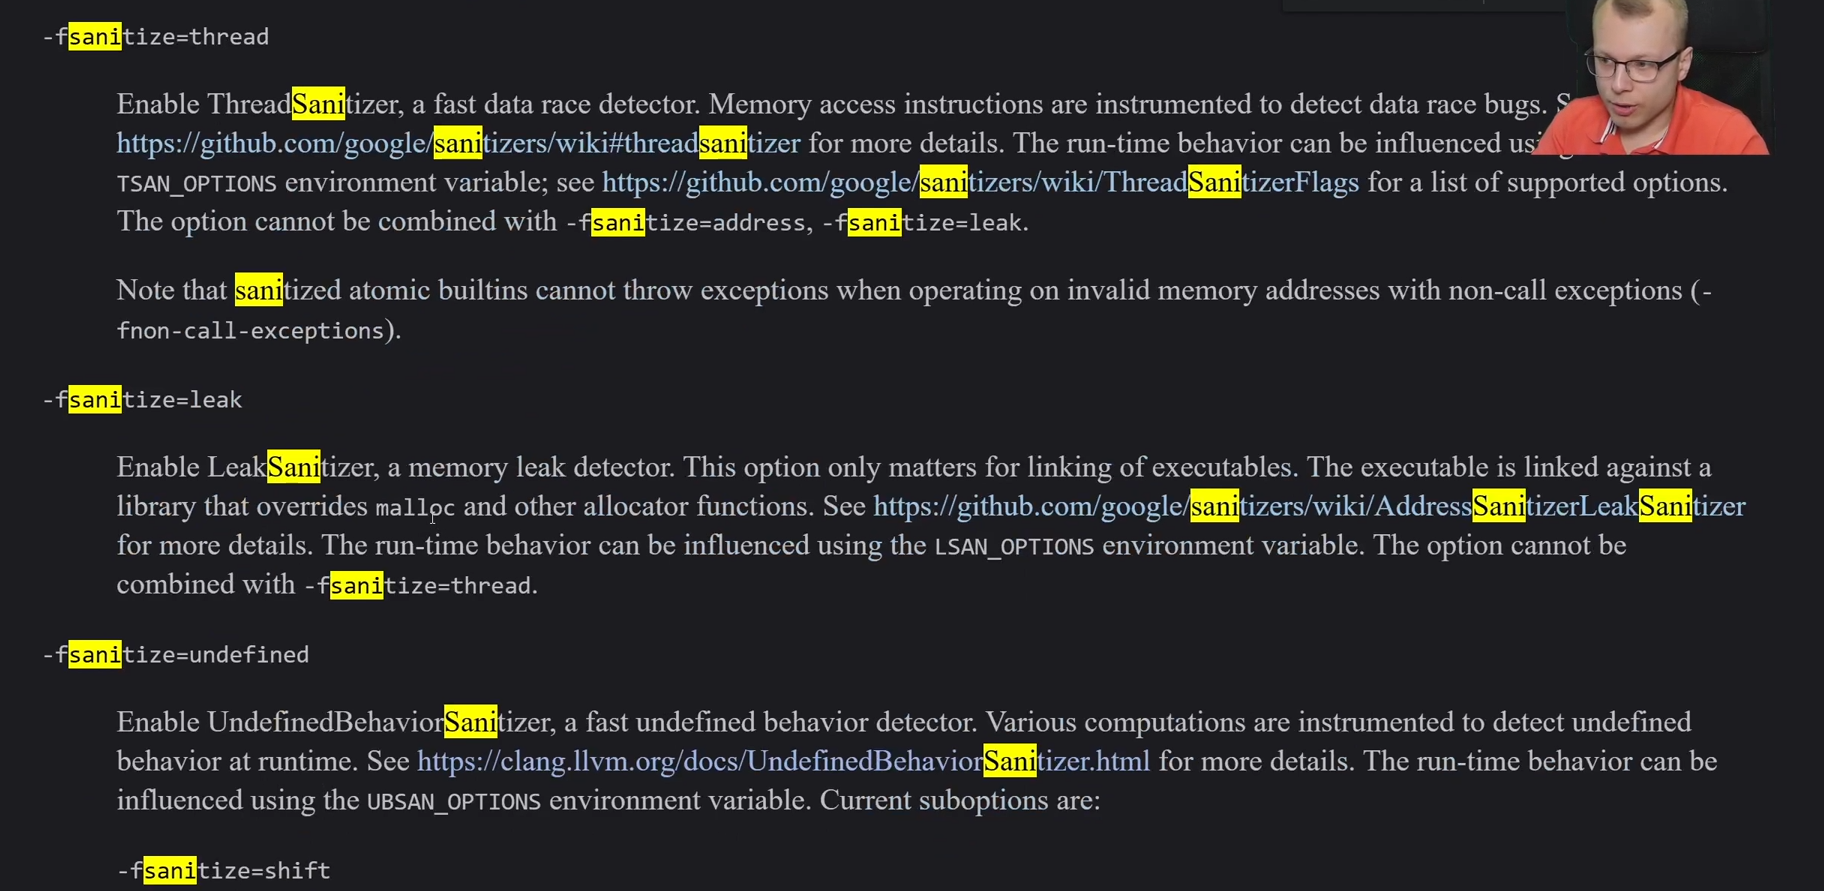
\includegraphics[width=5in]{fsan.png}
\end{center}


\begin{verbatim}
int main() {
    int x[2];
    x[2] = 1337;
}
\end{verbatim}

\section{IPO LTO}

In release mode, the release build, optimizations are activated to create the best product. C++ has many types of builds
for a project, debug modes, performance modes, etc. 

In this case, the release mode optimizations are related to the compiler for a better runtime. Yet, these optimizations
look at functions separately, not as a chain of functions so to speak (subsequent calls of different functions).

Link Time Optimization (LTO) or Interprocedural Optimization (IPO) [synonyms] is a response to these limits. Using functions from different translation units, the compiler with optimizations,
will be able to analyse them subsequently. In other words, the optimized compiler will be able to evaluate
if some operations can be cancelled in the function chain.

To use it, we will use a CMake function. All compilers (MSVC, CLANG and GCC) have LTO implemented.


\subsection{LTO Example - Clang}

\begin{verbatim}
--- a.h --- // .h for header file
            // this is genius note-taking!!!

extern int foo1(void);
extern void foo2(void);
extern void foo4(void);

--- a.c --- // .c for source file
            // this is genius note-taking!!!

#include "a.h"

static signed int i = 0;

void foo2(void {
    i = -1; 
}

static int foo3(void {
    i = -1; 
}

int foo1(void) {
    int data = 0;

    if (i < 0)
        data = foo3();

    data = data + 42;
    return data;
}

--- main.c ---
#include <stdio.h>
#include "a.h"

void foo4(void){
    printf("Hi\n");
}

int main() {
    return foo1()
}
\end{verbatim}

In this example, it is impossible for i to be reduced under zero. Since it is impossible, the foo3 function will never be
called. Thus, the compiler cancels an impossible chain and does not generate code for these logically uncallable functions.
This is the optimization.

\subsection{IPO LTO in CMake}

In your cmake directory, create a LTO.cmake file. Plus, create a new option in your root CMakelists.txt


\begin{verbatim}
option(ENABLE_LTO "Enable the link time optimization" ON)

...

if(ENABLE_LTO)
    include(LTO)
endif()
\end{verbatim}


\subsection{LTO.cmake}

Configuring link time optimization in the new lto.cmake file, in the cmake directory.

\begin{verbatim}
function(target_enable_lto TARGET ENABLE)
    if(NOT ${ENBALE})
    endif()

    include(CheckIPOSupported)
    check_ipo_supported(RESULT result OUTPUT output)

    if(result) 
        message(STATUS "IPO/LTO is supported!")
        set_property(TARGET ${TARGET} PROPERTY_INTERPROCEDURAL_OPTIMIZATION ${ENABLE})
    else()
        message("WARNING "IPO/LTO is not supported!")

                                     #PROPERTY... is a predefined variable in modern cmake
    endif()
endfunction(target_enable_lto)
\end{verbatim}

\subsection{LTO.cmake Refactoring}

The instructor revised the lto.cmake file at the end of the course.

\begin{verbatim}
function(target_enable_lto)         # he passes less arguments here
    set(oneValueArgs TARGET ENABLE)
    cmake_parse_arguments(          # every options and arguments in oneValueArgs
                                    # will be prefixed by LTO_
                                    # thus, TARGET becomes LTO_TARGET
        LTO
        "${options}"
        "${oneValueArgs}"
        "${multiValueArgs}"
        ${ARGN})


    include(CheckIPOSupported)
    check_ipo_supported(RESULT result OUTPUT output)

    if(result) 
        message(STATUS "IPO/LTO is supported: ${LTO_TARGET}")
        set_property(TARGET ${LTO_TARGET} PROPERTY_INTERPROCEDURAL_OPTIMIZATION ${LTO_ENABLE})
    else()
        message("WARNING "IPO/LTO is not supported! ${LTO_TARGET}")

                                     #PROPERTY... is a predefined variable in modern cmake
    endif()
endfunction(target_enable_lto)
\end{verbatim}

\subsection{In Our Target CMakeLists.txt}

Enabling LTO for our target library, means configuring it in its CMakeLists.txt file.

\begin{center}
    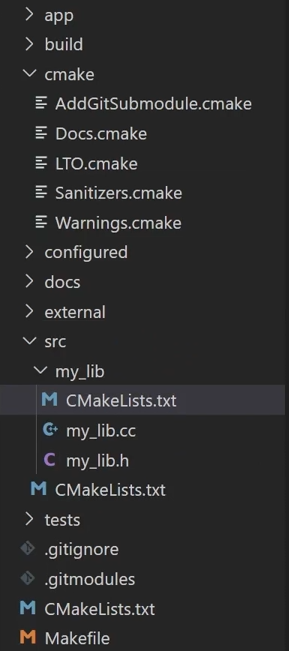
\includegraphics[width=2in]{lto_lib.png}
\end{center}


\begin{verbatim}
if(${ENABLE_LTO})
    target_enable_lto(${LIBRARY_NAME})
endif()

---- in app ----
---- CMakeLists.txt ----

if(${ENABLE_LTO})
    target_enable_lto(${EXECUTABLE_NAME} ${ENABLE_LTO})
endif()
\end{verbatim}

\chapter{Cpp Project Engineering}

A project template was included in the course. 


\section{Clang Tools}



\subsection{Clang Tools.cmake}

This content was seen at the end of the course. The instructor configured the tools in a new Tools.cmake file.


\begin{center}
    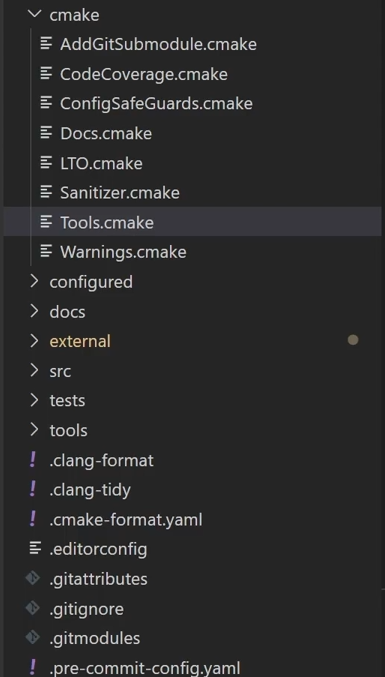
\includegraphics[width=2in]{tools_cm.png}
\end{center}


\begin{verbatim}
function(add_cmake_format_target)
    if(NOT ${ENABLE_CMAKE_FORMAT})
        return()
    endif()
    set(ROOT_CMAKE_FILES "${CMAKE_SOURCE_DIR}/CMakeLists.txt")
    file(GLOB_RECURSE CMAKE_FILES_TXT "*/CMakeLists.txt")
    file(GLOB_RECURSE CMAKE_FILES_C "cmake/*.cmake")
    list(
        FILTER
        CMAKE_FILES_TXT
        EXCLUDE
        REGEX
        "${CMAKE_SOURCE_DIR}/(build|external)/.*")
    set(CMAKE_FILES ${ROOT_CMAKE_FILES} ${CMAKE_FILES_TXT} ${CMAKE_FILES_C})
    find_program(CMAKE_FORMAT cmake-format)
    if(CMAKE_FORMAT)
        message(STATUS "Added Cmake Format")
        set(FORMATTING_COMMANDS)
        foreach(cmake_file ${CMAKE_FILES})
            list(
                APPEND
                FORMATTING_COMMANDS
                COMMAND
                cmake-format
                -c
                ${CMAKE_SOURCE_DIR}/.cmake-format.yaml
                -i
                ${cmake_file})
        endforeach()
        add_custom_target(
            run_cmake_format
            COMMAND ${FORMATTING_COMMANDS}
            WORKING_DIRECTORY ${CMAKE_SOURCE_DIR})
    else()
        message(WARNING "CMAKE_FORMAT NOT FOUND")
    endif()
endfunction()

function(add_clang_format_target)
    if(NOT ${ENABLE_CLANG_FORMAT})
        return()
    endif()
    find_package(Python3 COMPONENTS Interpreter)
    if(NOT ${Python_FOUND})
        return()
    endif()
    file(GLOB_RECURSE CMAKE_FILES_CC "*/*.cc")
    file(GLOB_RECURSE CMAKE_FILES_CPP "*/*.cpp")
    file(GLOB_RECURSE CMAKE_FILES_H "*/*.h")
    file(GLOB_RECURSE CMAKE_FILES_HPP "*/*.hpp")
    set(CPP_FILES
        ${CMAKE_FILES_CC}
        ${CMAKE_FILES_CPP}
        ${CMAKE_FILES_H}
        ${CMAKE_FILES_HPP})
    list(
        FILTER
        CPP_FILES
        EXCLUDE
        REGEX
        "${CMAKE_SOURCE_DIR}/(build|external)/.*")
    find_program(CLANGFORMAT clang-format)
    if(CLANGFORMAT)
        message(STATUS "Added Clang Format")
        add_custom_target(
            run_clang_format
            COMMAND
                ${Python3_EXECUTABLE}
                ${CMAKE_SOURCE_DIR}/tools/run-clang-format.py ${CPP_FILES}
                --in-place
            WORKING_DIRECTORY ${CMAKE_SOURCE_DIR}
            USES_TERMINAL)
    else()
        message(WARNING "CLANGFORMAT NOT FOUND")
    endif()
endfunction()

function(add_clang_tidy_to_target target)
    get_target_property(TARGET_SOURCES ${target} SOURCES)
    list(
        FILTER
        TARGET_SOURCES
        INCLUDE
        REGEX
        ".*.(cc|h|cpp|hpp)")

    find_package(Python3 COMPONENTS Interpreter)
    if(NOT ${Python_FOUND})
        message(WARNING "Python3 needed for Clang-Tidy")
        return()
    endif()

    find_program(CLANGTIDY clang-tidy)
    if(CLANGTIDY)
        if(CMAKE_CXX_COMPILER_ID MATCHES "MSVC")
            message(STATUS "Added MSVC ClangTidy (VS GUI only) for: ${target}")
            set_target_properties(
                ${target} PROPERTIES VS_GLOBAL_EnableMicrosoftCodeAnalysis
                                     false)
            set_target_properties(
                ${target} PROPERTIES VS_GLOBAL_EnableClangTidyCodeAnalysis true)
        else()
            message(STATUS "Added Clang Tidy for Target: ${target}")
            add_custom_target(
                ${target}_clangtidy
                COMMAND
                    ${Python3_EXECUTABLE}
                    ${CMAKE_SOURCE_DIR}/tools/run-clang-tidy.py
                    ${TARGET_SOURCES}
                    -config-file=${CMAKE_SOURCE_DIR}/.clang-tidy
                    -extra-arg-before=-std=${CMAKE_CXX_STANDARD}
                    -header-filter="\(src|app\)\/*.\(h|hpp\)"
                    -p=${CMAKE_BINARY_DIR}
                WORKING_DIRECTORY ${CMAKE_CURRENT_SOURCE_DIR}
                USES_TERMINAL)
        endif()
    else()
        message(WARNING "CLANGTIDY NOT FOUND")
    endif()
endfunction()
\end{verbatim}


\subsection{Clang Tool Directory}

The previous tool.cmake file references two python files, one for clang-format and one for clang-tidy.
Both are part of the LLVM package, no need to inspect those, it is part of the programs.

\begin{center}
    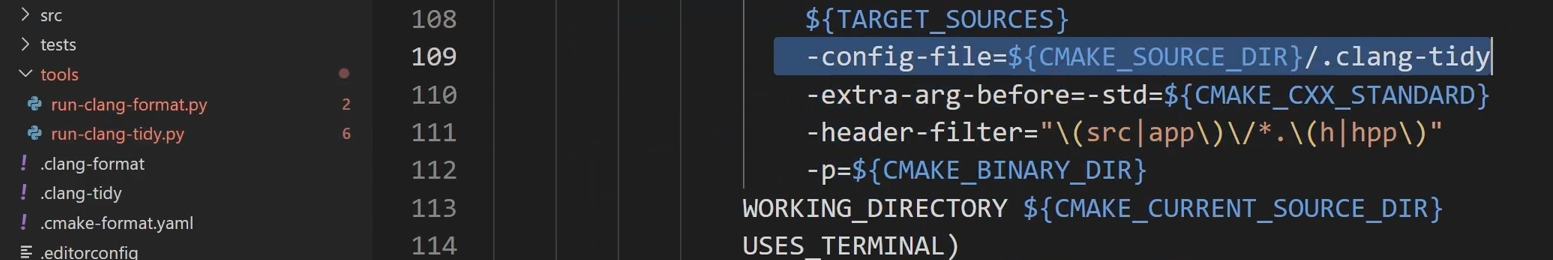
\includegraphics[width=2in]{runclang.png}
\end{center}

\subsection{Clang-Tidy}

A static linting tool for cpp, also known as static analyzers. It checks your code according
to set verifications. It is similar to compile warnings, but a linter does not require any compilation
to run. It checks to code whenever needed.


You do not need to use the clang compiler to use it.


It is nice to use, because it is the earliest form of warnings. It saves a ton of time if you do not have to compile
to have warnings. Early on is best.


\textbf{Use clang-tidy's modernize-loop-convert check} for range based loops.


\begin{verbatim}
Documentation for Clang-Tidy: https://clang.llvm.org/extra/clang-tidy/
\end{verbatim}


\subsection{.clang-tidy file}

Specify the checks clang-tidy executes in a .clang-tidy file at the root of your project.

\begin{verbatim}
Checks: 'clang-analyzer-*,cppcoreguidelines-*,
        modernize-*,bugprone-*,performance-*,readability-non-const-parameter,
        misc-const-correctness,misc-use-anonymous-namespace,
        google-explicit-constructor,-modernize-use-trailing-return-type,
        -bugprone-exception-escape,-cppcoreguidelines-pro-bounds-constant-array-index,
        -cppcoreguidelines-avoid-magic-numbers,-bugprone-easily-swappable-parameters'


        # modernize-* --------------- includes all warnings in this category
        # -bugprone=exception-escape # - with a '-' char, 
                                     # specifies one omition in the group

WarningsAsErrors: ''
HeaderFilterRegex: '\(src|app\)\/*.\(h|hpp\)'
AnalyzeTemporaryDtors: false
FormatStyle:     none
\end{verbatim}


\subsection{Clang-tidy Target}

Configuring a target for clang-tidy checks is made possible in the target's CMakeLists.txt. Here, in my\_lib dir
for library, our target.


\begin{verbatim}
if(${ENABLE_CLANG_TIDY})
    add_clang_tidy_to_target(${LIBA}) # this is defined in the Tools.cmake file
endif()
\end{verbatim}

\subsection{Clang-tidy in root CMakeLists.txt}

Create an option for clang-tidy in your projects' root CMakeLists.txt

\begin{verbatim}
option(ENABLE_CLANG_TIDY "Enable to add clang tidy." ON)


set(CMAKE_EXPOET_COMPILE_COMMANDS ON) # this cmake function creates a json file
                                      # clang-tidy needs this json to work
                                      # to differenciate your code from dependencies.

\end{verbatim}


\subsection{Clang-tidy on Microsoft MSVC}

To activate it with the microsoft compiler, you need to use the Visual Studio Code GUI only.
Some filters, defined in .clang-tidy config file may not work on Windows, but will work on Unix systems.

\begin{center}
    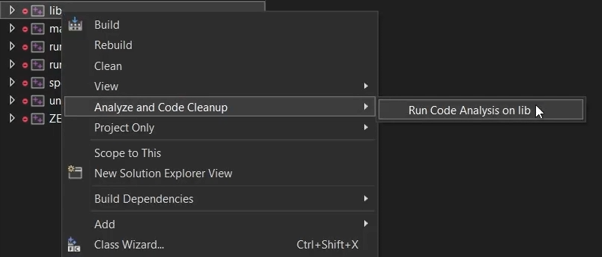
\includegraphics[width=2in]{ms_tidy.png}
\end{center}

 
\subsection{Clang-Format}

An essential professional formatting tool for cpp. Use version 14 at least, 16+ is best. The 
clang-tidy and clang-format .py files expects at least clang-format 14. Command line arguments 
change with versions. Check cpp project template .clang-format file in root directory.

Plus, these tools were configured in the root CMakeLists.txt file.

\begin{verbatim}
Documentation for Clang-Format: https://clang.llvm.org/docs/ClangFormat.html

Install Clang Tools

It's included in the LLVM toolchain, but also installable by apt, brew, winget etc.

https://github.com/llvm/llvm-project/releases/tag/llvmorg-16.0.0
\end{verbatim}


\subsection{Clang-Format Configuration in Tools.cmake}


\begin{verbatim}
function(add_clang_format_target)
    if(NOT ${ENABLE_CLANG_FORMAT})
        return()
    endif()
    find_package(Python3 COMPONENTS Interpreter)
    if(NOT ${Python_FOUND})
        return()
    endif()
    file(GLOB_RECURSE CMAKE_FILES_CC "*/*.cc")
    file(GLOB_RECURSE CMAKE_FILES_CPP "*/*.cpp")
    file(GLOB_RECURSE CMAKE_FILES_H "*/*.h")
    file(GLOB_RECURSE CMAKE_FILES_HPP "*/*.hpp")
    set(CPP_FILES
        ${CMAKE_FILES_CC}
        ${CMAKE_FILES_CPP}
        ${CMAKE_FILES_H}
        ${CMAKE_FILES_HPP})
    list(
        FILTER
        CPP_FILES
        EXCLUDE
        REGEX
        "${CMAKE_SOURCE_DIR}/(build|external)/.*") 

                                # exclude build and external files

    find_program(CLANGFORMAT clang-format)
    if(CLANGFORMAT)
        message(STATUS "Added Clang Format")
        add_custom_target(
            run_clang_format
            COMMAND
                ${Python3_EXECUTABLE}
                ${CMAKE_SOURCE_DIR}/tools/run-clang-format.py ${CPP_FILES}
                --in-place
            WORKING_DIRECTORY ${CMAKE_SOURCE_DIR}
            USES_TERMINAL)
    else()
        message(WARNING "CLANGFORMAT NOT FOUND")
    endif()
endfunction()
\end{verbatim}

\subsection{CMake-Format}

A nice-to-have .cmake file formater. It may make your project easier to read, 
since it standardizes all of your CMakeLists.txt files and .
Check .cmake-format.yaml file in root directory.

Plus, these tools were configured in the root CMakeLists.txt file.


\begin{center}
    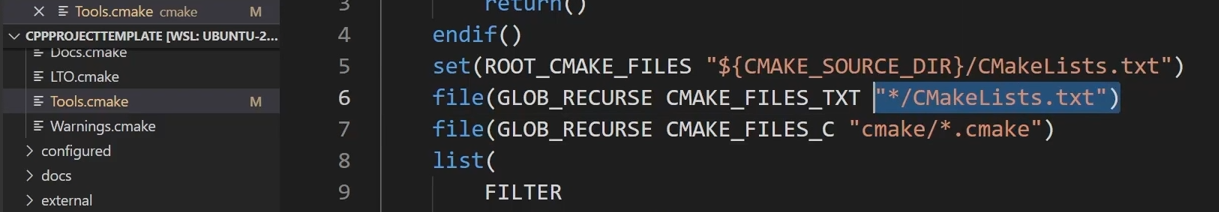
\includegraphics[width=2in]{tools4.png}
\end{center}


\begin{verbatim}
Install CMake-format,

pip install cmake-format # python 3.7+
\end{verbatim}


\subsection{CMake-Format Configuration in Tools.cmake}


\begin{verbatim}
function(add_cmake_format_target)
    if(NOT ${ENABLE_CMAKE_FORMAT})
        return()
    endif()
    set(ROOT_CMAKE_FILES "${CMAKE_SOURCE_DIR}/CMakeLists.txt")
    file(GLOB_RECURSE CMAKE_FILES_TXT "*/CMakeLists.txt")
    file(GLOB_RECURSE CMAKE_FILES_C "cmake/*.cmake")
    list(
        FILTER
        CMAKE_FILES_TXT
        EXCLUDE
        REGEX
        "${CMAKE_SOURCE_DIR}/(build|external)/.*")
    set(CMAKE_FILES ${ROOT_CMAKE_FILES} ${CMAKE_FILES_TXT} ${CMAKE_FILES_C})
    find_program(CMAKE_FORMAT cmake-format)
    if(CMAKE_FORMAT)
        message(STATUS "Added Cmake Format")
        set(FORMATTING_COMMANDS)
        foreach(cmake_file ${CMAKE_FILES})
            list(
                APPEND
                FORMATTING_COMMANDS
                COMMAND
                cmake-format
                -c                     # this flag finds the config flag. 
                                       # this is the file.
                ${CMAKE_SOURCE_DIR}/.cmake-format.yaml

                -i                     # specifies to replace the file in-place.
                                       # Otherwise, like sed command,
                                       # it only outputs the file
                ${cmake_file})
        endforeach()
        add_custom_target(
            run_cmake_format
            COMMAND ${FORMATTING_COMMANDS}
            WORKING_DIRECTORY ${CMAKE_SOURCE_DIR})
    else()
        message(WARNING "CMAKE_FORMAT NOT FOUND")
    endif()
endfunction()
\end{verbatim}

\subsection{Glob and Exclude Cmake Functions}

For clang and cmake-format tools, the tools.cmake file contains globing functions to
find all .cmake and CMakeLists.txt files.


\begin{center}
    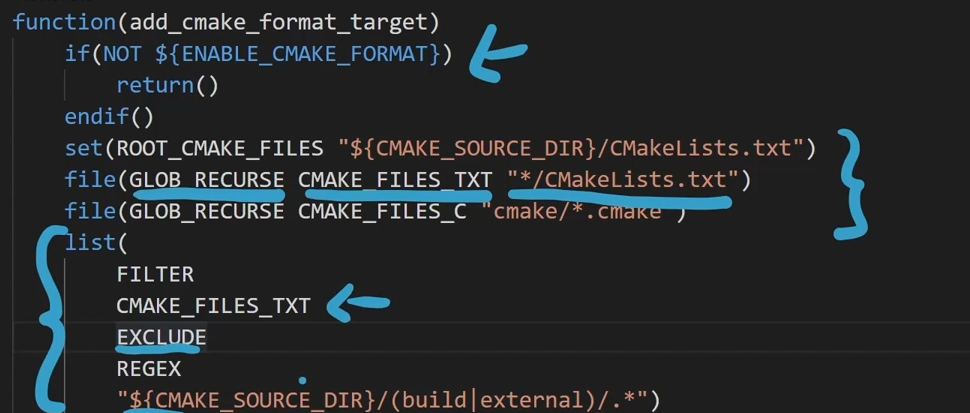
\includegraphics[width=2in]{glob.png}
\end{center}

\subsection{Github Pages}

Since Doxygen creates an html you can have a github-pages branch of your project and
use github pages to create a webpage your project.

In your .github directory of you project, in a workflows directory, create a documentation.yaml file. 
This will configure github to update your doc webpage automatically.


\begin{center}
    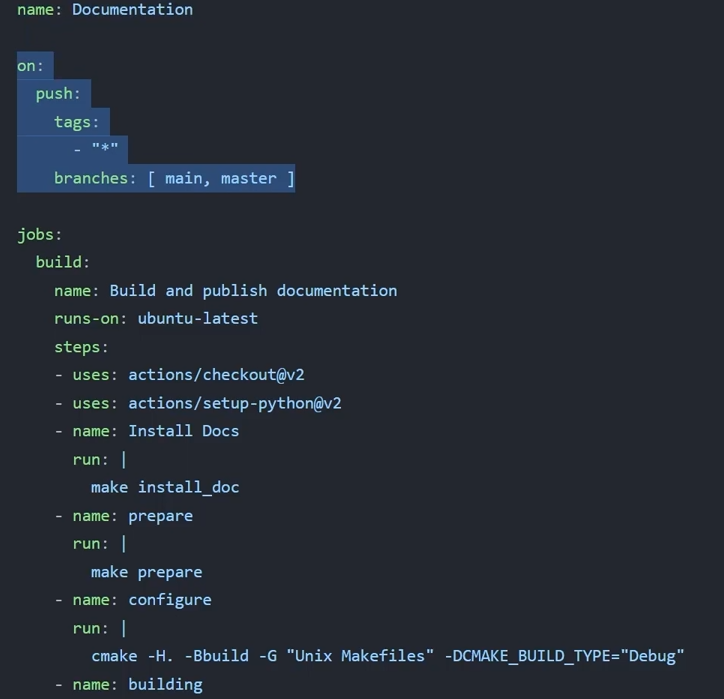
\includegraphics[width=2in]{pages.png}
\end{center}

Then, when we push to master, all the jobs will be run by github.

\begin{verbatim}
name: Documentation

on:
  push:
    tags:
      - "*"
    branches: [ main, master ]

jobs:
  build:
    name: Build and publish documentation
    runs-on: ubuntu-latest
    steps:
    - uses: actions/checkout@v2
    - uses: actions/setup-python@v2
    - name: Install Docs
      run: |
        sudo apt-get install doxygen
        pip install jinja2 Pygments
    - name: prepare
      run: |
        make prepare
    - name: configure
      run: |
        cmake -H. -Bbuild -G "Unix Makefiles" -DCMAKE_BUILD_TYPE="Debug"
    - name: building
      run: |
        cmake --build build --config Debug --target docs -j4
    - name: Deploy to GitHub Pages
      uses: Cecilapp/GitHub-Pages-deploy@v3
      env:
        GITHUB_TOKEN: ${{ secrets.GITHUB_TOKEN }}
      with:
        build_dir: ./docs/html   # where is the doxygen documentation
\end{verbatim}

It hosts the website on MikaelJG.github.io/repo-name/. Public documentation uploaded online.

\section{Code Coverage}

A metric to know how many lines of code were tested by our unit tests.
These tools are only available in linux.

\begin{verbatim}
sudo apt-get install gcovr lcov
\end{verbatim}

\subsection{Code Coverage Configuration in root CMakeLists.txt}

\begin{verbatim}
option(ENABLE_COVERAGE "Enable a Code COverage build." ON)

...

if(ENABLE_COVERAGE)
    include(CodeCoverage)
    append_coverage_compiler_flags() # defined in CodeCoverage.cmake file
endif()

\end{verbatim}

\subsection{Code Coverage for target library in my lib CMakeLists.txt}

Configure code coverage for a specific target in its CMakeLists.txt file.

\begin{verbatim}
if(ENABLE_COVERAGE)
    set(COVERAGE_MAIN "coverage") # the name of this coverage to run
    set(COVERAGE_EXCLUDES
        "${PROJECT_SOURCE_DIR}/app/*"
        "${PROJECT_SOURCE_DIR}/cmake/*"
        "${PROJECT_SOURCE_DIR}/docs/*"
        "${PROJECT_SOURCE_DIR}/external/*"
        "${PROJECT_SOURCE_DIR}/tests/*"
        "${PROJECT_SOURCE_DIR}/build/*"
        "$usr/indlude/*")
    setup_target_for_coverage_lcov(
        NAME
        ${COVERAGE_MAIN}
        EXECUTABLE
        ${UNIT_TEST_NAME}
        DEPENDENCIES
        ${UNIT_TEST_NAME})
endif()
\end{verbatim}


\subsection{Code Coverage Directory}

lcov generates a code Coverage directory, with information in an html.


\begin{center}
    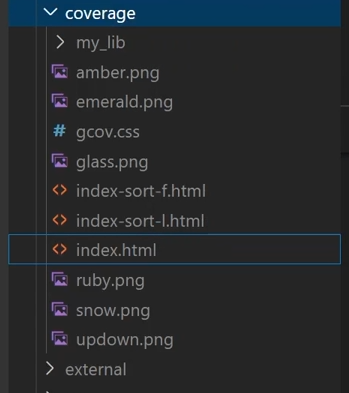
\includegraphics[width=2in]{cov.png}
\end{center}


\begin{center}
    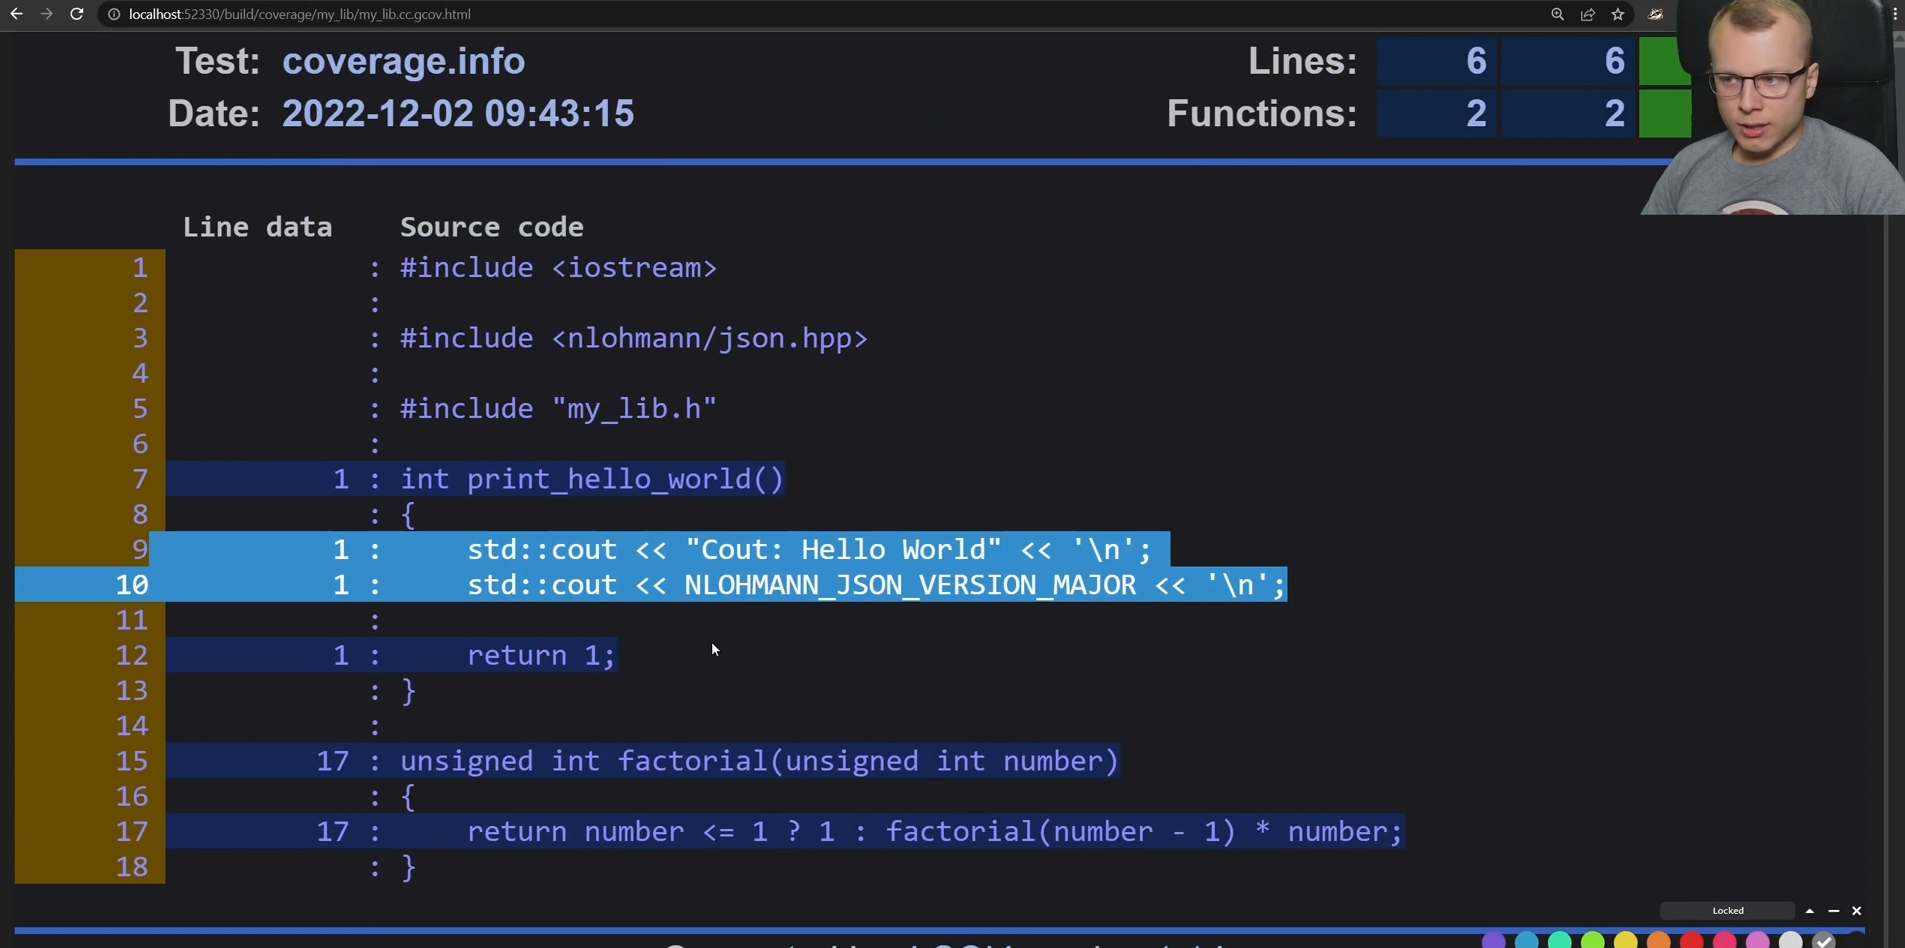
\includegraphics[width=2in]{cov2.png}
\end{center}



\subsection{Code Coverage.cmake}

\begin{verbatim}
include(CMakeParseArguments)

if(ENABLE_COVERAGE)
    # Check prereqs
    find_program(GCOV_PATH gcov)
    find_program(
        LCOV_PATH
        NAMES lcov
              lcov.bat
              lcov.exe
              lcov.perl)
    find_program(GENHTML_PATH NAMES genhtml genhtml.perl genhtml.bat)
    find_program(GCOVR_PATH gcovr PATHS ${CMAKE_SOURCE_DIR}/scripts/test)
    find_program(CPPFILT_PATH NAMES c++filt)

    if(NOT GCOV_PATH)
        message(FATAL_ERROR "gcov not found! Aborting...")
    endif() # NOT GCOV_PATH

    if(CMAKE_C_COMPILER_ID MATCHES "Clang" OR CMAKE_CXX_COMPILER_ID MATCHES
                                              "Clang")
        set(IS_CLANG TRUE)
    else()
        set(IS_CLANG FALSE)
    endif()
    if(CMAKE_C_COMPILER_ID MATCHES "GNU" OR CMAKE_CXX_COMPILER_ID MATCHES "GNU")
        set(IS_GCC TRUE)
    else()
        set(IS_GCC FALSE)
    endif()

    if(NOT ${IS_CLANG} AND NOT ${IS_GCC})
        message(FATAL_ERROR "Compiler is not gcc/clang! Aborting...")
    endif()

    set(COVERAGE_COMPILER_FLAGS "-g -O0 -fprofile-arcs -ftest-coverage")
    set(CMAKE_CXX_FLAGS_COVERAGE ${COVERAGE_COMPILER_FLAGS} FORCE)
    set(CMAKE_C_FLAGS_COVERAGE ${COVERAGE_COMPILER_FLAGS} FORCE)
    set(CMAKE_EXE_LINKER_FLAGS_COVERAGE "-lgcov" FORCE)
    set(CMAKE_SHARED_LINKER_FLAGS_COVERAGE "" FORCE)
    mark_as_advanced(
        CMAKE_CXX_FLAGS_COVERAGE
        CMAKE_C_FLAGS_COVERAGE
        CMAKE_EXE_LINKER_FLAGS_COVERAGE
        CMAKE_SHARED_LINKER_FLAGS_COVERAGE)

    if(NOT
       CMAKE_BUILD_TYPE
       STREQUAL
       "Debug")
        message(WARNING "Cov results with non-Debug build may be misleading")
    endif()

    if(${IS_GCC})
        link_libraries(gcov)
    endif()
endif()

# Defines a target for running and collection code coverage information Builds
# dependencies, runs the given executable and outputs reports. NOTE! The
# executable should always have a ZERO as exit code otherwise the coverage
# generation will not complete.
#
function(setup_target_for_coverage_lcov)
    set(options NO_DEMANGLE)
    set(oneValueArgs BASE_DIRECTORY NAME)
    set(multiValueArgs
        EXCLUDE
        EXECUTABLE
        EXECUTABLE_ARGS
        DEPENDENCIES
        LCOV_ARGS
        GENHTML_ARGS)
    cmake_parse_arguments(
        Coverage
        "${options}"
        "${oneValueArgs}"
        "${multiValueArgs}"
        ${ARGN})

    if(NOT LCOV_PATH)
        message(FATAL_ERROR "lcov not found! Aborting...")
    endif()
    if(NOT GENHTML_PATH)
        message(FATAL_ERROR "genhtml not found! Aborting...")
    endif()

    # Set base directory (as absolute path), or default to PROJECT_SOURCE_DIR
    if(${Coverage_BASE_DIRECTORY})
        get_filename_component(BASEDIR ${Coverage_BASE_DIRECTORY} ABSOLUTE)
    else()
        set(BASEDIR ${PROJECT_SOURCE_DIR})
    endif()

    # Collect excludes (CMake 3.4+: Also compute absolute paths)
    set(LCOV_EXCLUDES "")
    foreach(EXCLUDE ${Coverage_EXCLUDE} ${COVERAGE_EXCLUDES}
                    ${COVERAGE_LCOV_EXCLUDES})
        if(CMAKE_VERSION VERSION_GREATER 3.4)
            get_filename_component(
                EXCLUDE
                ${EXCLUDE}
                ABSOLUTE
                BASE_DIR
                ${BASEDIR})
        endif()
        list(APPEND LCOV_EXCLUDES "${EXCLUDE}")
    endforeach()
    list(REMOVE_DUPLICATES LCOV_EXCLUDES)

    # Conditional arguments
    if(CPPFILT_PATH AND NOT ${Coverage_NO_DEMANGLE})
        set(GENHTML_EXTRA_ARGS "--demangle-cpp")
    endif()

    # Setup target
    add_custom_target(
        ${Coverage_NAME}
        # Cleanup lcov
        COMMAND ${LCOV_PATH} ${Coverage_LCOV_ARGS} --gcov-tool ${GCOV_PATH}
                -directory . -b ${BASEDIR} --zerocounters
        # Create baseline to make sure untouched files show up in the report
        COMMAND ${LCOV_PATH} ${Coverage_LCOV_ARGS} --gcov-tool ${GCOV_PATH} -c
                -i -d . -b ${BASEDIR} -o ${Coverage_NAME}.base
        # Run tests
        COMMAND ${Coverage_EXECUTABLE} ${Coverage_EXECUTABLE_ARGS}
        # Capturing lcov counters and generating report
        COMMAND
            ${LCOV_PATH} ${Coverage_LCOV_ARGS} --gcov-tool ${GCOV_PATH}
            --directory . -b ${BASEDIR} --capture --output-file
            ${Coverage_NAME}.capture
        # add baseline counters
        COMMAND
            ${LCOV_PATH} ${Coverage_LCOV_ARGS} --gcov-tool ${GCOV_PATH} -a
            ${Coverage_NAME}.base -a ${Coverage_NAME}.capture --output-file
            ${Coverage_NAME}.total
        # filter collected data to final coverage report
        COMMAND
            ${LCOV_PATH} ${Coverage_LCOV_ARGS} --gcov-tool ${GCOV_PATH} --remove
            ${Coverage_NAME}.total ${LCOV_EXCLUDES} --output-file
            ${Coverage_NAME}.info
        # Generate HTML output
        COMMAND ${GENHTML_PATH} ${GENHTML_EXTRA_ARGS} ${Coverage_GENHTML_ARGS}
                -o ${Coverage_NAME} ${Coverage_NAME}.info
        # Set output files as GENERATED (will be removed on 'make clean')
        BYPRODUCTS ${Coverage_NAME}.base
                   ${Coverage_NAME}.capture
                   ${Coverage_NAME}.total
                   ${Coverage_NAME}.info
                   ${Coverage_NAME} # report directory
        WORKING_DIRECTORY ${PROJECT_BINARY_DIR}
        DEPENDS ${Coverage_DEPENDENCIES}
        VERBATIM # Protect arguments to commands
    )

    # Show where to find the lcov info report
    add_custom_command(
        TARGET ${Coverage_NAME}
        POST_BUILD
        COMMAND ;)

    # Show info where to find the report
    add_custom_command(
        TARGET ${Coverage_NAME}
        POST_BUILD
        COMMAND ;)
endfunction()

function(append_coverage_compiler_flags)
    set(CMAKE_C_FLAGS
        "${CMAKE_C_FLAGS} ${COVERAGE_COMPILER_FLAGS}"
        PARENT_SCOPE)
    set(CMAKE_CXX_FLAGS
        "${CMAKE_CXX_FLAGS} ${COVERAGE_COMPILER_FLAGS}"
        PARENT_SCOPE)
    message(
        STATUS
            "Appending code coverage compiler flags: ${COVERAGE_COMPILER_FLAGS}"
    )
endfunction()
\end{verbatim}


\section{Github Actions Continuous Integration}

Yml files instruct github to perform some actions when you push to the main branch. 
You can have unit testing automatically when you push for example.


\begin{center}
    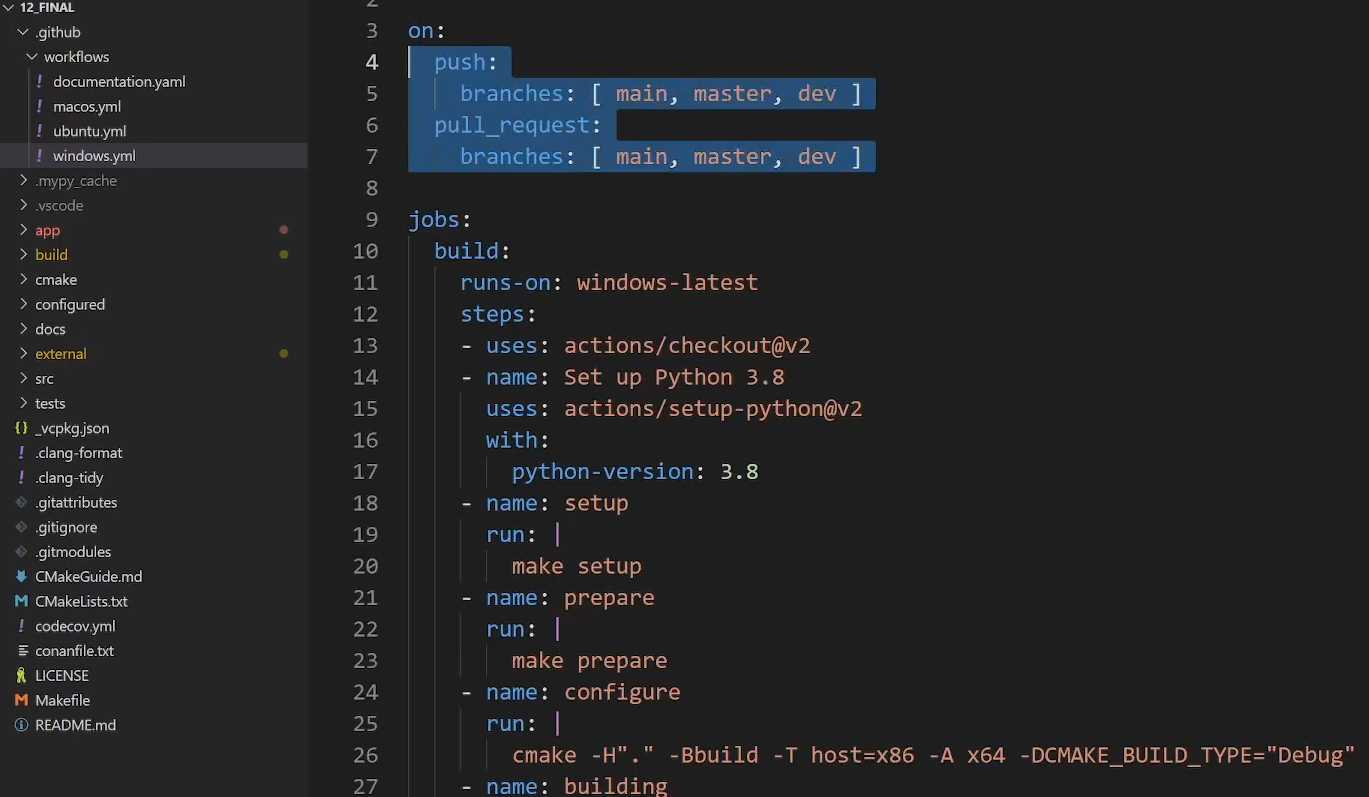
\includegraphics[width=4in]{actions.png}
\end{center}

For Ubuntu, you can have automatic code coverage as well. Not possible on macOS and Windows.


\subsection{Github Actions Workflows}

Follow your workflows, your different configurated unit tests on Github.


\begin{center}
    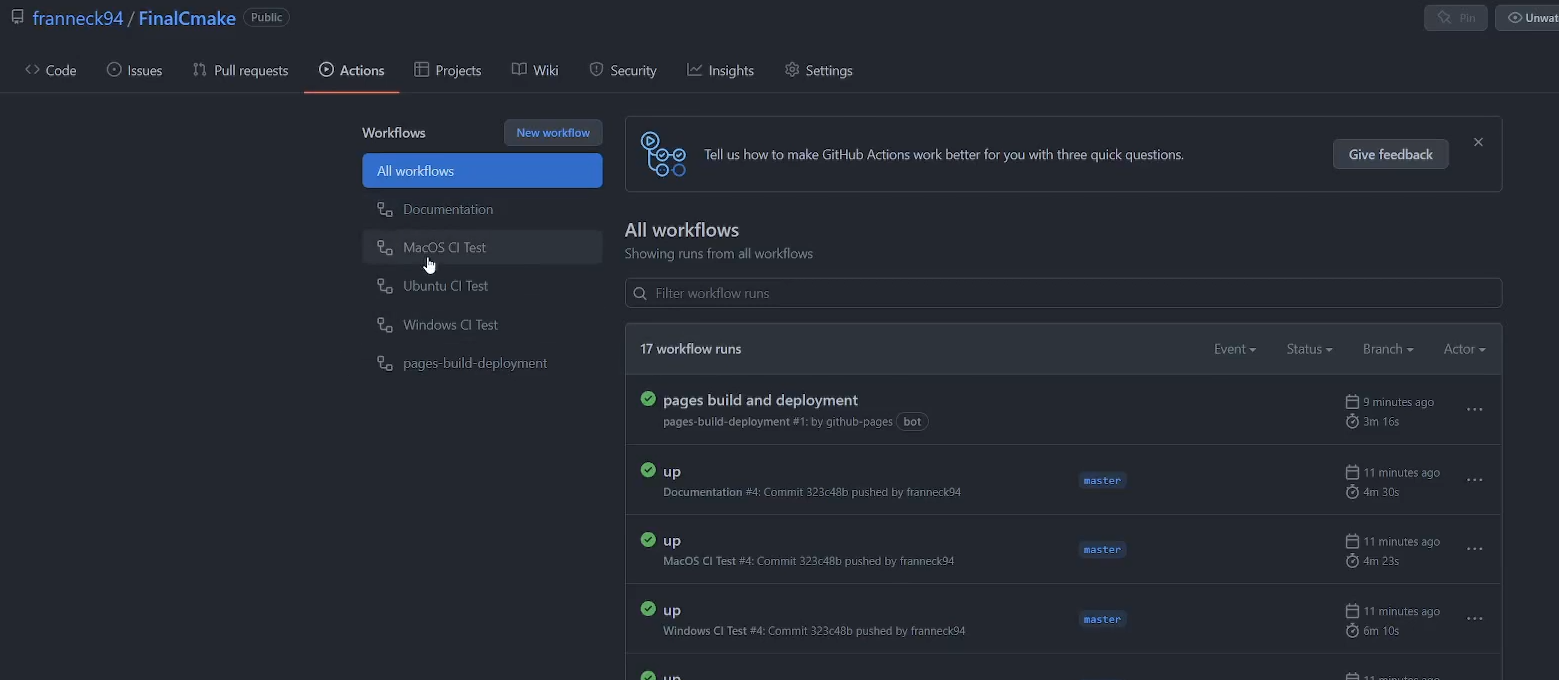
\includegraphics[width=2in]{actions2.png}
\end{center}

For every job configured, every step is executed on github, with a checkmark if everything has passed.


\begin{center}
    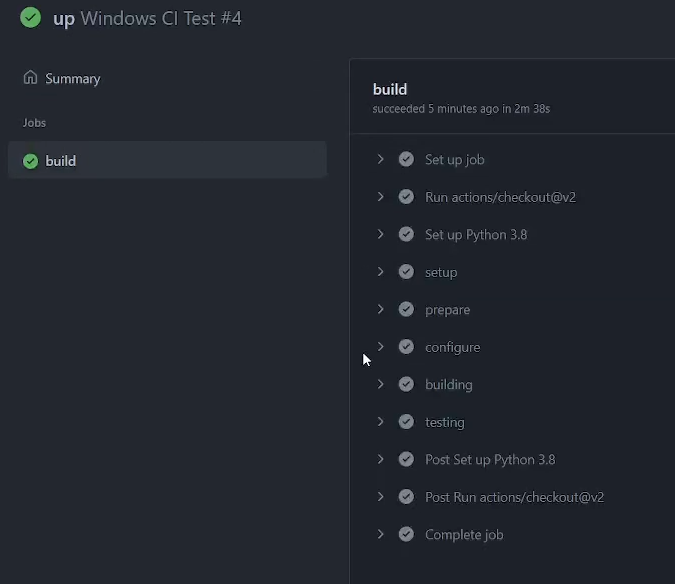
\includegraphics[width=2in]{actions3.png}
\end{center}

You can have great icons to see versions of the project passing on your github page.


\begin{center}
    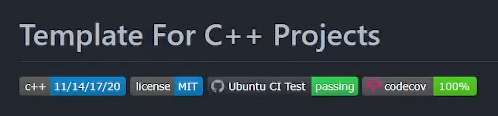
\includegraphics[width=2in]{actions4.png}
\end{center}


\begin{center}
    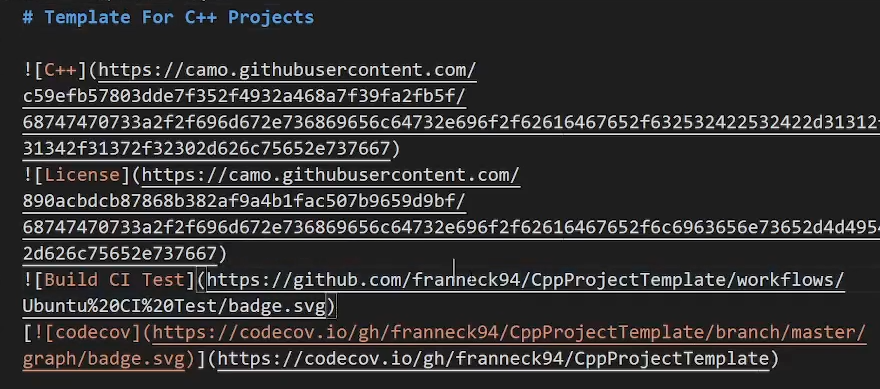
\includegraphics[width=2in]{actions5.png}
\end{center}


\subsection{Github Actions Codecov}

In Ubuntu, it is possible to upload the code coverage online, for free, automatically with github actions.

\begin{center}
    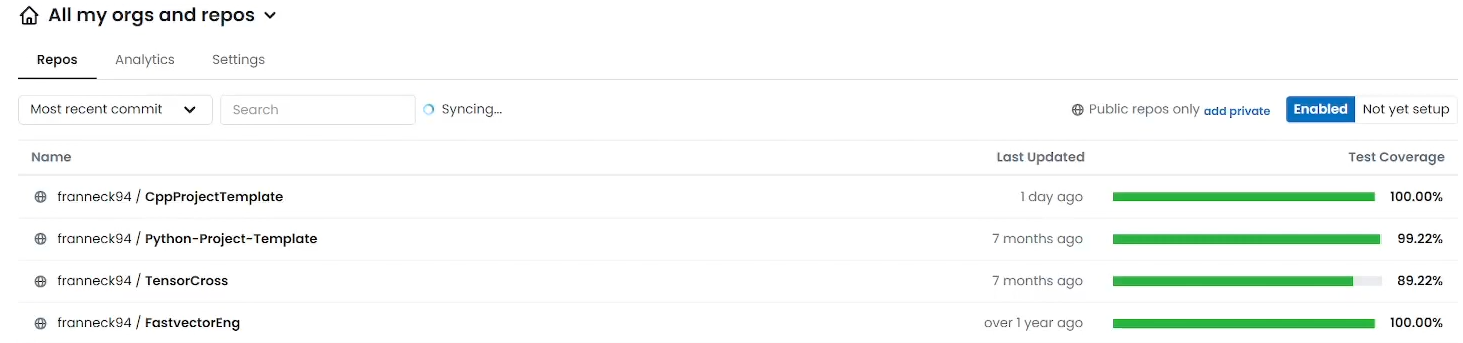
\includegraphics[width=2in]{codecov.png}
\end{center}

It is based on the Ubuntu.yaml configuration file.

\begin{center}
    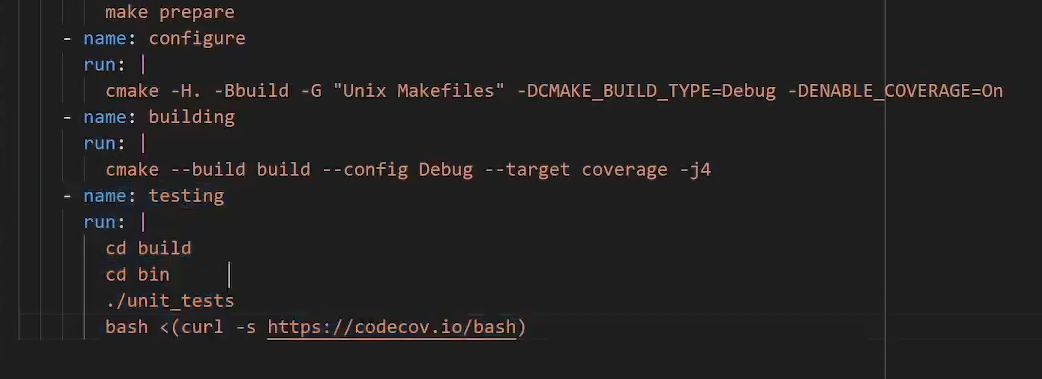
\includegraphics[width=2in]{codecov2.png}
\end{center}



\section{Pre-Commit}

When you have a github repo with your cpp project, you have many config files. Technically,
a user doesn't have to use any of your tools. However, there is a way to force him to do so, with 
Pre-Commit.


\subsection{Pre-Commit Installation}

Install pre-commit, a python program, with pip.

\begin{verbatim}
pip install pre-commit
\end{verbatim}


\subsection{Pre-Commit Configuration}

In your root directory, create a .pre-commit-config.yaml file.

\begin{verbatim}
fail_fast: false
repos:
-   repo: https://github.com/pre-commit/pre-commit-hooks
    rev: v4.4.0
    hooks:
      - id: check-yaml
      - id: check-json
        exclude: .vscode
      - id: end-of-file-fixer
      - id: trailing-whitespace

-   repo: https://github.com/pre-commit/mirrors-clang-format
    rev: 'v16.0.3'
    hooks:
      - id: clang-format
        exclude_types: [javascript, json]
\end{verbatim}

Then, run \$pre-commit install and \$pre-commit install-hooks commands from the project root.


\subsection{Pre-Commit in GitHub Actions Workflow Directory}

You can run Pre-Commit everytime there is a push on github branches with a pre-commit.yaml in the .github/workflow 
directory. It will run pre-commit on all pull requests as well!

\begin{verbatim}
name: pre-commit

on:
    pull_request:
    push:
        branches: [ main, master ]

jobs:
    pre-commit:
        runs-on: ubuntu-latest
        steps:
        - uses: actions/checkout@v2
        - uses: actions/setup python@v2
        - uses: pre-commit/action@2.0.0
\end{verbatim}


\section{Install Command for your Program}

We can make our build executable usable on your computer, just like any other tool. To make a transition from 
our project to our real computer, we will use an install command.


\subsection{Install in root CMakeLists.txt}

On linux, cmake install automatically on usr/local. On windows, it is in Programs directory.

\begin{verbatim}
install(TARGETS ${HE}
    EXPORT ${LIBA}
    ARCHIVE DESTINATION lib
    LIBRARY DESTINATION lib
    RUNTIME DESTINATION bin) 

install(TARGETS ${LIBA}
        ARCHIVE DESTINATION lib
        LIBRARY DESTINATION lib)

# in build

$ sudo cmake --build . --target install
\end{verbatim}


\begin{center}
    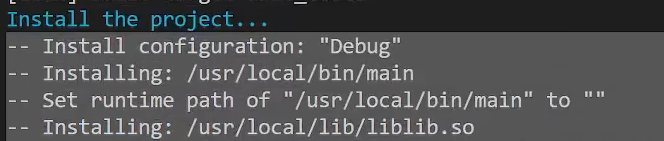
\includegraphics[width=2in]{inst.png}
\end{center}

\subsection{Install any CMake Program on the Internet}

Logically, you could clone any Cmake project from github, build it and use the executable as a regular
program on your machine. This is how pros do it, I guess.


\begin{verbatim}
Clone the repo
Generate the Cmake project (cmake --build ...)
and
Run the install function we just seen.
\end{verbatim}

\section{Jason Turner's Template}

\begin{verbatim}
lefticus/cmake_template // Jason Turner 2023 cmake starter pack

rename "myproject" in the cmake files to use it.

\end{verbatim}

\subsection{Jason Turner Tools Defaults- ProjectOptions.cmake}

\begin{verbatim}
Address sanitizer
Undefined behavior sanitizer
Fuzzing example built
Procedural optimization IPO (link time optimization)
Warnings as errors
Clang-tidy enabled
CPPcheck enabled
Options for precompiled headers
\end{verbatim}

\subsection{Hardening - Hardening.cmake}

\begin{verbatim}
Hardened compilation // make code safer
More compilation options / securities.

-fstack-protector
-fcf-protection
-fsanitize=undefined // undefined behavior sanitizer
-fno-sanitize-recover=undefined
-fsanitizise-minimal-runtime

+ debug information 
\end{verbatim}


\section{CMake Vim Plugins Combos}

\begin{verbatim}
See codevion/cpp2.md
\end{verbatim}

\section{COC - for code completion in nvim}
\begin{verbatim}
https://github.com/neoclide/coc.nvim
Jason Turner has this too
\end{verbatim}

\subsection{Pragma Once}

\begin{verbatim}
#pragma once is a non-standard directive that serves as an include guard. 
It ensures that a header file is included only once during the compilation process,
regardless of how many times it is referenced.

Placed at the beginning of a header file, it acts as a compiler directive to prevent multiple inclusions
Supported by most compilers, including GCC, Clang, and MSVC.
\end{verbatim}

\subsection{Glob - Include Many files with CMake}
 
You have at least two options. First, include every files one-by-one in the CMakeList.txt.
\begin{verbatim}
cmake_minimum_required(VERSION 3.10)
set(CMAKE_CXX_STANDARD 17)
set(CMAKE_CXX_STANDARD_REQUIRED ON)

project(hello VERSION 1.0) // traditional way to include files
add_executable(hello main.cpp Blah.cpp) // added here
target_include_directories(hello PUBLIC ${CMAKE_CURRENT_SOURCE_DIR}/include)
\end{verbatim}

Cmake discourages this glob method, but it is a more sane options for large projects.

\begin{verbatim}
file(GLOB_RECURSE SRC_FILES src/*.cpp) // glob everything in src/
add_executable(hello ${SRC_FILES})
\end{verbatim}

\textbf{In CMake - Traditionally Added}
\begin{verbatim}
add_executable(hello main.cpp src/Blah.cpp) // added here
\end{verbatim}

\textbf{In CMake - Globing}
\begin{verbatim}
file(GLOB_RECURSE SRC_FILES src/*.cpp)
add_executable(hello main.cpp ${SRC_FILES})
\end{verbatim}

\section{Jason Turner's CMake Template - Options}

\begin{verbatim}
include(cmake/SystemLink.cmake)
include(cmake/LibFuzzer.cmake)
include(CMakeDependentOption)
include(CheckCXXCompilerFlag)

macro(myproject_supports_sanitizers)
  if((CMAKE_CXX_COMPILER_ID MATCHES ".*Clang.*" OR CMAKE_CXX_COMPILER_ID MATCHES ".*GNU.*") AND NOT WIN32)
    set(SUPPORTS_UBSAN ON)
  else()
    set(SUPPORTS_UBSAN OFF)
  endif()

  if((CMAKE_CXX_COMPILER_ID MATCHES ".*Clang.*" OR CMAKE_CXX_COMPILER_ID MATCHES ".*GNU.*") AND WIN32)
    set(SUPPORTS_ASAN OFF)
  else()
    set(SUPPORTS_ASAN ON)
  endif()
endmacro()

macro(myproject_setup_options)
  option(myproject_ENABLE_HARDENING "Enable hardening" ON)
  option(myproject_ENABLE_COVERAGE "Enable coverage reporting" OFF)
  cmake_dependent_option(
    myproject_ENABLE_GLOBAL_HARDENING
    "Attempt to push hardening options to built dependencies"
    ON
    myproject_ENABLE_HARDENING
    OFF)

  myproject_supports_sanitizers()

  if(NOT PROJECT_IS_TOP_LEVEL OR myproject_PACKAGING_MAINTAINER_MODE)
    option(myproject_ENABLE_IPO "Enable IPO/LTO" OFF)
    option(myproject_WARNINGS_AS_ERRORS "Treat Warnings As Errors" OFF)
    option(myproject_ENABLE_USER_LINKER "Enable user-selected linker" OFF)
    option(myproject_ENABLE_SANITIZER_ADDRESS "Enable address sanitizer" OFF)
    option(myproject_ENABLE_SANITIZER_LEAK "Enable leak sanitizer" OFF)
    option(myproject_ENABLE_SANITIZER_UNDEFINED "Enable undefined sanitizer" OFF)
    option(myproject_ENABLE_SANITIZER_THREAD "Enable thread sanitizer" OFF)
    option(myproject_ENABLE_SANITIZER_MEMORY "Enable memory sanitizer" OFF)
    option(myproject_ENABLE_UNITY_BUILD "Enable unity builds" OFF)
    option(myproject_ENABLE_CLANG_TIDY "Enable clang-tidy" OFF)
    option(myproject_ENABLE_CPPCHECK "Enable cpp-check analysis" OFF)
    option(myproject_ENABLE_PCH "Enable precompiled headers" OFF)
    option(myproject_ENABLE_CACHE "Enable ccache" OFF)
  else()
    option(myproject_ENABLE_IPO "Enable IPO/LTO" ON)
    option(myproject_WARNINGS_AS_ERRORS "Treat Warnings As Errors" ON)
    option(myproject_ENABLE_USER_LINKER "Enable user-selected linker" OFF)
    option(myproject_ENABLE_SANITIZER_ADDRESS "Enable address sanitizer" ${SUPPORTS_ASAN})
    option(myproject_ENABLE_SANITIZER_LEAK "Enable leak sanitizer" OFF)
    option(myproject_ENABLE_SANITIZER_UNDEFINED "Enable undefined sanitizer" ${SUPPORTS_UBSAN})
    option(myproject_ENABLE_SANITIZER_THREAD "Enable thread sanitizer" OFF)
    option(myproject_ENABLE_SANITIZER_MEMORY "Enable memory sanitizer" OFF)
    option(myproject_ENABLE_UNITY_BUILD "Enable unity builds" OFF)
    option(myproject_ENABLE_CLANG_TIDY "Enable clang-tidy" ON)
    option(myproject_ENABLE_CPPCHECK "Enable cpp-check analysis" ON)
    option(myproject_ENABLE_PCH "Enable precompiled headers" OFF)
    option(myproject_ENABLE_CACHE "Enable ccache" ON)
  endif()

  if(NOT PROJECT_IS_TOP_LEVEL)
    mark_as_advanced(
      myproject_ENABLE_IPO
      myproject_WARNINGS_AS_ERRORS
      myproject_ENABLE_USER_LINKER
      myproject_ENABLE_SANITIZER_ADDRESS
      myproject_ENABLE_SANITIZER_LEAK
      myproject_ENABLE_SANITIZER_UNDEFINED
      myproject_ENABLE_SANITIZER_THREAD
      myproject_ENABLE_SANITIZER_MEMORY
      myproject_ENABLE_UNITY_BUILD
      myproject_ENABLE_CLANG_TIDY
      myproject_ENABLE_CPPCHECK
      myproject_ENABLE_COVERAGE
      myproject_ENABLE_PCH
      myproject_ENABLE_CACHE)
  endif()

  myproject_check_libfuzzer_support(LIBFUZZER_SUPPORTED)
  if(LIBFUZZER_SUPPORTED AND (myproject_ENABLE_SANITIZER_ADDRESS OR myproject_ENABLE_SANITIZER_THREAD OR myproject_ENABLE_SANITIZER_UNDEFINED))
    set(DEFAULT_FUZZER ON)
  else()
    set(DEFAULT_FUZZER OFF)
  endif()

  option(myproject_BUILD_FUZZ_TESTS "Enable fuzz testing executable" ${DEFAULT_FUZZER})

endmacro()

macro(myproject_global_options)
  if(myproject_ENABLE_IPO)
    include(cmake/InterproceduralOptimization.cmake)
    myproject_enable_ipo()
  endif()

  myproject_supports_sanitizers()

  if(myproject_ENABLE_HARDENING AND myproject_ENABLE_GLOBAL_HARDENING)
    include(cmake/Hardening.cmake)
    if(NOT SUPPORTS_UBSAN 
       OR myproject_ENABLE_SANITIZER_UNDEFINED
       OR myproject_ENABLE_SANITIZER_ADDRESS
       OR myproject_ENABLE_SANITIZER_THREAD
       OR myproject_ENABLE_SANITIZER_LEAK)
      set(ENABLE_UBSAN_MINIMAL_RUNTIME FALSE)
    else()
      set(ENABLE_UBSAN_MINIMAL_RUNTIME TRUE)
    endif()
    message("${myproject_ENABLE_HARDENING} ${ENABLE_UBSAN_MINIMAL_RUNTIME} ${myproject_ENABLE_SANITIZER_UNDEFINED}")
    myproject_enable_hardening(myproject_options ON ${ENABLE_UBSAN_MINIMAL_RUNTIME})
  endif()
endmacro()

macro(myproject_local_options)
  if(PROJECT_IS_TOP_LEVEL)
    include(cmake/StandardProjectSettings.cmake)
  endif()

  add_library(myproject_warnings INTERFACE)
  add_library(myproject_options INTERFACE)

  include(cmake/CompilerWarnings.cmake)
  myproject_set_project_warnings(
    myproject_warnings
    ${myproject_WARNINGS_AS_ERRORS}
    ""
    ""
    ""
    "")

  if(myproject_ENABLE_USER_LINKER)
    include(cmake/Linker.cmake)
    configure_linker(myproject_options)
  endif()

  include(cmake/Sanitizers.cmake)
  myproject_enable_sanitizers(
    myproject_options
    ${myproject_ENABLE_SANITIZER_ADDRESS}
    ${myproject_ENABLE_SANITIZER_LEAK}
    ${myproject_ENABLE_SANITIZER_UNDEFINED}
    ${myproject_ENABLE_SANITIZER_THREAD}
    ${myproject_ENABLE_SANITIZER_MEMORY})

  set_target_properties(myproject_options PROPERTIES UNITY_BUILD ${myproject_ENABLE_UNITY_BUILD})

  if(myproject_ENABLE_PCH)
    target_precompile_headers(
      myproject_options
      INTERFACE
      <vector>
      <string>
      <utility>)
  endif()

  if(myproject_ENABLE_CACHE)
    include(cmake/Cache.cmake)
    myproject_enable_cache()
  endif()

  include(cmake/StaticAnalyzers.cmake)
  if(myproject_ENABLE_CLANG_TIDY)
    myproject_enable_clang_tidy(myproject_options ${myproject_WARNINGS_AS_ERRORS})
  endif()

  if(myproject_ENABLE_CPPCHECK)
    myproject_enable_cppcheck(${myproject_WARNINGS_AS_ERRORS} "" # override cppcheck options
    )
  endif()

  if(myproject_ENABLE_COVERAGE)
    include(cmake/Tests.cmake)
    myproject_enable_coverage(myproject_options)
  endif()

  if(myproject_WARNINGS_AS_ERRORS)
    check_cxx_compiler_flag("-Wl,--fatal-warnings" LINKER_FATAL_WARNINGS)
    if(LINKER_FATAL_WARNINGS)
      # This is not working consistently, so disabling for now
      # target_link_options(myproject_options INTERFACE -Wl,--fatal-warnings)
    endif()
  endif()

  if(myproject_ENABLE_HARDENING AND NOT myproject_ENABLE_GLOBAL_HARDENING)
    include(cmake/Hardening.cmake)
    if(NOT SUPPORTS_UBSAN 
       OR myproject_ENABLE_SANITIZER_UNDEFINED
       OR myproject_ENABLE_SANITIZER_ADDRESS
       OR myproject_ENABLE_SANITIZER_THREAD
       OR myproject_ENABLE_SANITIZER_LEAK)
      set(ENABLE_UBSAN_MINIMAL_RUNTIME FALSE)
    else()
      set(ENABLE_UBSAN_MINIMAL_RUNTIME TRUE)
    endif()
    myproject_enable_hardening(myproject_options OFF ${ENABLE_UBSAN_MINIMAL_RUNTIME})
  endif()

endmacro()
\end{verbatim}

\end{document}







\chapter{GDB - GNU Debugger}

\section{Keywords}

\begin{verbatim}
Seen commands:
info gdb 					//Manual
info locals 				        //Vars in local scope
info variables				//Vars declared outside current scope
info functions				//Names and datatypes of all defined functions
info b 						//List all breakpoints
break funcName				//Set breakpoint at function funcName (short: b funcName)
break file::line			        //Set breakpoint at line in file
layout next					//Cycle through the layouts of gdb
p var 						//Print the value of variable var
p var = value 			        	//Force set value to a var
run 						        //Start the program
start 						//Synonymous to (b main && run). Puts temporary b at main
next 						//Execute the current line in source (short: n)
step 						//Step into function call at current line (short: s)
finish						//Finish the execution of current function (short: fin)
continue					//Resume execution (After a breakpoint) (short: c)
refresh 					        //Repaint the interface (To fix corrupted interface)
shell cmd 					//Run shell command cmd from gdb prompt
python gdb.execute(cmd)		//Run a gdb command cmd from python prompt
set print pretty on			//Enable pretty printing
							  (Put in ~/.gdbinit)
$ gdb -c core.num			//Examine the dumped core file from a SIGSEGV(shell command)
bt							//Print backtrace
break _exit 				        //Breakpoint at exit of program
whatis expr					//Print datatype of expr
ptype expr					//Detailed print of datatype of expr
watch var 					//Stop when var is modified
watch -l foo				        //Watch foo loaction
rwatch foo					//Stop when foo is read
watch foo if foo>10			//Watch foo conditionally
delete						//Delete all breakpoints
delete breakpoint_no		        //Delete breakpoint breakpoint_no
command breakpoint_no		//Run user listed commands when breakpoint is hit
							  (End list of commands with 'end')
file executable 			        //Load the executable for debugging from inside gdb
quit						        //Quit (short: q)

Feel free to correct/add any useful command you know.
\end{verbatim}

\chapter{Engineering}
\section{Builds}

\subsection{Build Configuration (build target)}

\begin{verbatim}
    Project settings determining how your project will be built. 
    Build configuration includes executable name, project arch and library files. 
    It specifies keepings or strippings of debugging info, compiler optimization details 
\end{verbatim}

\subsection{Build Release Configuration}

\begin{verbatim}
    Optimized for size and performance, no debugging information.
    With all optimization, now testing for code performance.

    When the Hello World program (from lesson 0.7) was built using Visual Studio,
    Executable produced in the debug configuration was 65kb, 
    Executable built in the release version was 12kb. 
    The difference is largely due to the extra debugging information kept in the debug build.
\end{verbatim}


\subsection{Build Testing Configuration}

\begin{verbatim}
    Debug configuations turns off all optimizations, includes debugging information,
    Jason Turner would say "with as much information as possible"
    Such configs makes your programs larger and slower, but much easier to debug. 
\end{verbatim}

\subsection{G++ Builds}
\begin{verbatim}
GCC / Clang? 
    -ggdb  // cmd line debugging
           // This is the GNU Debugger !?
    -ggdb O2 -DNDEBUG for release builds. ??
    -g++ O2 -DNDEBUG for release builds. ??
\end{verbatim}

\section{Debugging}

\begin{verbatim}
    Debug configuations turns off all optimizations, includes debugging information,
    Jason Turner would say "with as much information as possible"
    Such configs makes your programs larger and slower, but much easier to debug. 
\end{verbatim}

\section{GDB}
\section{Testing Framework Catch2}

\section{Benchmarking}
\section{Threads}


\end{document}
